Why Python?  It is flexible, freely available and cross platform.  It is easy 
 to learn and well documented.   There are numerous online tutorials, for example at: http://docs.python.org/tutorial/ or this new (and very excellent) one: http://www.python-course.eu/index.php.  
There are lots of numerical, statistical and visualization packages.  Finally, it is 
easy to install.  Really.  Go to:  

http://www.enthought.com/products/edudownload.php, 

\noindent
supply your academic e-mail address and follow the instructions.  The only potentially tricky bit is setting your path properly.   To do this, just put the following line at the end of  your .cshrc file:

{\singlespacing \color{blue} \begin{verbatim}
set path = (/Library/Frameworks/Python.framework/Versions/Current/bin/ $path)
\end{verbatim}}

\noindent
To make sure you have installed Python properly, simply type:
{\singlespacing \color{blue} \begin{verbatim}
% python   
\end{verbatim}}
\noindent
You should get something that looks like this:

{\singlespacing \color{blue} \begin{verbatim}
Enthought Python Distribution -- www.enthought.com
Version: 7.1-2 (32-bit)

Python 2.7.2 |EPD 7.1-2 (32-bit)| (default, Jul 27 2011, 13:29:32) 
[GCC 4.0.1 (Apple Inc. build 5493)] on darwin
Type "packages", "demo" or "enthought" for more information.
>>> 
\end{verbatim}   }
\noindent
If you don't get something about Enthought Python, you are probably using the standard Mac Os version, which has none of the whistles and bells we want (plotting, numerical packages, etc.), so start over with the Introduction.    Otherwise, we are ready to begin!

\section{An Interactive Python session}

As you have just fired up Python, you are in an interactive mode with the prompt  {\color{blue}$>>>$}.  Like Matlab, you can just start typing commands. After each command, press the return key and see what happens:

{\singlespacing \color{blue} \begin{verbatim}
>>> a=2 
>>> a
2
>>> b=2
>>> c=a+b
>>> c
>>> c+=1
>>> c
5
>>> a=2; b=2; c=a+b; c
4
>>> d,e,f=4,5,6 # note syntax! d=4;e=5;f=6
>>> # note also that the symbol '#' means the rest of the line is a comment!
\end{verbatim}}

To get out of Python interactive mode and back to your beloved command line, type the control key (here-after  {\color{blue}\^{ }}) and  {\color{blue}D} at the same time.  PC users may have to type {\color{blue} \^{ }C} instead. 

From your Fortran programming experience, you will recognize $a, b,$ and $c$ in the above session as {\it variables} and $+$ as an {\it operation}. You may have been surprised that we didn't declare variables up front (C programmers always have to).  And, the variables above are obviously behaving as integers, not floating point variables (no decimals) but they are not letters between $i$ and $n$.  And there were funny lines that seemed to set three numbers at once:

{\singlespacing \color{blue} \begin{verbatim}
>>> a=2; b=2; c=a+b; c
and
>>> d,e,f=4,5,6 # note syntax! d=4;e=5;f=6
\end{verbatim}}
\noindent
Here are some rules governing variables and operations in Python:


\begin{itemize}
\item Variable names are composed of alphanumeric characters, including `-` and '\_'.
\item They are case sensitive:  `a' is not the same as 'A'.
\item They do NOT have to be specified in advance (unlike C)
\item In fortran, integers are  $i-n$ and floating points are all else - not the case in Python. You can make them whatever you want.  
\item + adds, - subtracts, * multiplies, / divides, \% gives the remainder, ** raises to the power
\item These two are fun: {\color{blue}+=} and  {\color{blue}-=}.  They increment and decrement respectively. 
\item Parentheses determine order of operation (as in Fortran). 
\item  For math functions, we can use various modules that either come standard with python (the math module) or are additions that come with the Enthought Python Edition we are using (the NumPy module).  A module is just a collection of functions. NB:  There is online help for any python function or method:  just type help(FUNC). 
\end{itemize}


\section{A first look at NumPy}

O.K.  First of all - how do you pronounce `NumPy'.  According to Important People at Enthought (e.g, Robert Kern), it should be pronounced ``Num'' as in ``Number'' and ``Pie'' as in, well, pie, or Python.  Oops.  It is way more fun to say Numpee!

So, that out of the way, what can NumPy do for us?  Turns out, a whole heck of a lot!  But for now we will just scratch the surface.   It can, for example, give us the value of $\pi$ as {\color{blue}numpy.pi}.  Note how the module name comes first, then the name of the function we wish to use.  In this case, the function just returns the value of $\pi$.  

To use {\color{blue}NumPy} functions, we must first ``import'' the module with the command {\color{blue}import}.  The first time you do this after installing Python, it may take a while, but after that it should be very quick.  

There are four styles of the import command which all do pretty much the same thing but differ in how you have to call the function after importing: 

{\singlespacing \color{blue} \begin{verbatim}
>>>  import numpy
>>> numpy.pi
3.1415926535897931
\end{verbatim}}
\noindent
This makes all the functions in NumPy available to you, but you have to call them with the {\color{blue}numpy.FUNC} syntax.

{\singlespacing \color{blue} \begin{verbatim}
>>>  import numpy as np  # or anything else!  e.g., some use:  N
>>> np.pi  # or N.pi in the second case.
3.1415926535897931
\end{verbatim}}
\noindent
This does the same as the first, but allows you to call NumPy anything you want - to save typing?
\noindent
To import all the functions from NumPy and not have to type numpy at all: 
{\singlespacing \color{blue} \begin{verbatim}
>>> from numpy  import *
>>> pi
3.1415926535897931
\end{verbatim}}
\noindent
This imports all the umpty-ump functions, which is a heavy load on your memory,  but you can also just import a few, like {\color{blue}pi} or {\color{blue}sqrt}:
{\singlespacing \color{blue} \begin{verbatim}
>>> from numpy import pi, sqrt # pi and square root
>>> pi
3.1415926535897931
>>> sqrt(4)
2.0
\end{verbatim}
}
\noindent
Did you notice how {\color{blue}sqrt(4)} where 4 was an integer, returned a floating point variable (2.0)?  

{\color{magenta}Good housekeeping Tip \#1:  I tend to import modules using the first option above.  That way  I know what module the functions I'm using are coming from - especially because we don't know off-hand ALL the functions available in any given module and there might be conflicts with my own function names or two different modules could have the same function (like} {\color{blue}math} {\color{magenta}and }{\color{blue}numpy}).  


Here is a (partial) list of some useful {\color{blue}NumPy} functions:


\begin{tabular}{ll}
\hline
absolute(x)  & absolute value\\
arccos(x)    & arccosine\\
arcsin(x)    & arcsine\\
arctan(x)    & arctangent\\
arctan2(y,x)  &arctangent of y/x in correct quadrant (***very useful!)\\
cos(x)        &cosine\\
cosh(x)      & hyperbolic cosine\\
exp(x)      &  exponential\\
log(x)      &  natural logarithm\\
log10(x)    &  base 10 log\\
sin(x)       & sine\\
sinh(x)     &  hyperbolic sine\\
sqrt(x)    &   square root\\
tan(x)      &  tangent\\
tanh(x)    &   hyperbolic tangent\\
\hline
\end{tabular}

\noindent 
Note that  in the trigonometric functions,  the argument is in RADIANS!.You can convert from degrees to radians by multiplying by:  {\color{blue}numpy.pi/180.}.  Also notice how these functions have parentheses, as opposed to {\color{blue}numpy.pi} which has none.  The difference is that these take arguments, while  {\color{blue}numpy.pi} just returns the value of $\pi$.  


\noindent 
If you are desperate, you can always use your Python interpreter as a calculator:

{\singlespacing \color{blue} \begin{verbatim}
>>> import numpy
>>> a=2
>>> b=-12
>>> c=16
>>> quad1 = (-b + numpy.sqrt(b**2-4.*a*c))/(2.*a)
>>> quad1
4
>>> y=numpy.sin(numpy.pi/6.)
>>> y
0.5
\end{verbatim}}


\section{Variable types}

The time has come to talk about variable types.  We've been very relaxed up to now, because we don't have to declare them up front and we can often even change them from one type to another on the fly.  But - variable types matter, so here goes.  Like Fortran, Python has integer, floating point (both long and short), string and complex variable types.  It is pretty clever about figuring out what is required.   Here are some examples:

{\singlespacing \color{blue} \begin{verbatim}
>>> number=1 # an integer
>>> Number=1.0 # a floating point
>>> NUMBER='1' # a string
>>> complex=1j # a complex number with imaginary part 1
>>> complex(3,1) # the complex number 3+1i 
\end{verbatim}}
\noindent
{Try doing math with these!}
{\singlespacing \color{blue} \begin{verbatim}
>>> number+number
2     [ an integer]
>>> number+Number
2.0   [ a float]
>>> NUMBER+NUMBER
11 [a string]
>>> number+NUMBER  [Gives you an angry error message]
\end{verbatim}}
\noindent
 Lesson learned: you can't add a number and a string.  and string addition is different!  But you really have to be careful with this.  If you multiply a float by an integer, it is possible that you will convert the float to an integer when you really wanted all those numbers after the decimal! So, if you want a float, use a float.  
 
{ You can convert from one type to another (if appropriate) with:}
{\singlespacing \color{blue} \begin{verbatim} 
 int(Number); str(number);  float(NUMBER); 
 long(Number); complex(real,imag)
 \end{verbatim}}
 
\noindent 
{\color{blue}long()} converts to a double precision floating point and {\color{blue}complex()} converts the two parts to a complex number.
 
 There is another kind of variable called ``boolean''. These are: {\color{blue}true}, {\color{blue}false}, {\color{blue}and}, {\color{blue}or}, and {\color{blue}not}
For the record, the integer  `1' is {\color{blue}true} and  `0' is {\color{blue}false}.  
These can be used to control the flow of the program as we shall learn later.  

\section{Data Structures}

In Fortran, you encountered arrays, which was a nice way to group a sequence of numbers that belonged together.  In Python of course we also have arrays, but we also have more complicated data structures, like lists, tuples, and dictionaries,  that group arbitrary variables together, like strings and integers and floats - whatever you want really. We'll go through some attributes of the various data structures, starting with lists.

\subsection{Lists}
%%\vskip -.25in
\begin{itemize}
\item Lists are denoted with []  and can contain any arbitrary set of items, including other lists!
\item Items in the list are referred to by an index number, starting with 0.  Note that this is different from Fortran which starts counting in arrays with the number 1.
\item You can  count from the end to the beginning by starting with -1 (the last item in the list), -2 (second to last), etc. 
\item Items can be sorted, deleted, inserted, sliced, counted, concatenated, replaced, added on, etc.
\end{itemize}
\noindent
Examples:

{\singlespacing \color{blue} \begin{verbatim}
>>> mylist=[`a',2.0,`400',`spam',42,[24,2]] # defines a list
>>> mylist[2] # refers to the third item
`400'
>>> mylist[-1] # refers to the last item
[24,2]
>>> mylist[1]=26.3   # replaces the second item
>>> del mylist[3] # deletes the fourth element 
\end{verbatim}}


\noindent
To slice out a chunk of the middle of a list:
{\singlespacing \color{blue} \begin{verbatim}
>>> newlist=mylist[1:3]
\end{verbatim}}
\noindent
This takes items 2 and 3 out (note it takes out up to but not including the last item number - don't ask me why).  
Or, we can slice it this way:
{\singlespacing \color{blue} \begin{verbatim}
>>> newlist=mylist[3:] 
\end{verbatim}}
\noindent
which takes from the fourth item (starting from 0!) to the end. 


To copy a list BEWARE! You can make  a copy - but it isn't a copy like in Fortran, but it is just another name for the SAME OBJECT, so:
{\singlespacing \color{blue} \begin{verbatim}
>>> mycopy=mylist
>>>mylist[2]=`new'
>>>mycopy[2]
`new'
\end{verbatim}}
\noindent
See how mycopy got changed when we changed mylist?
\noindent
To spawn a new list that is a copy, but an independent entity:
{\singlespacing \color{blue} \begin{verbatim}
>>>mycopy=mylist[:]
\end{verbatim}}
\noindent
Now try:
{\singlespacing \color{blue} \begin{verbatim}
>>>mylist[2]=1003
>>>mycopy[2]
`new'
\end{verbatim}}
\noindent
So now {\color{blue}mycopy}  stayed the way it was, even as {\color{blue}mylist } changed.  


Unlike Fortran, Python is ``object oriented'', a popular concept in coding circles.  We'll learn more about what that means later, but for right now you can walk around feeling smug that you are learning an object oriented programming language.   O.K., what is an object?  Well, 
{\color{blue}mylist} is an object.   Cool.  What do objects have that might be handy?  
Objects have ``methods'' which allow you to do things to them.  Methods have the form:
{\color{blue}object.method()}

\noindent
Here are two examples:

{\singlespacing \color{blue} \begin{verbatim}
>>> mylist.append(`me too') # appends a string to mylist
>>> mylist.sort() # sorts the list alphanumerically
>>> mylist
[2.0, 42, [24, 2], '400', 'a', 'me too', 'spam']
\end{verbatim}}
%%\vskip .25in


\noindent

 For a complete list of methods for lists, see:
http://docs.python.org/tutorial/datastructures.html\#more-on-lists

\subsection{More about strings}
Numbers are numbers. While there are more kinds of numbers (complex, etc.),
strings can be  more interesting. Unlike in Fortran, they can be denoted with single, double or triple quotes:  e.g.,
`spam',  ``Sam's spam'', or
{\singlespacing \color{blue} \begin{verbatim}
"""  
Hi there I can type as
many lines as I want
"""
\end{verbatim}}

Strings can be added together ({\color{blue}newstring = 'spam' + 'alot'}).  They  can be sliced ({\color{blue}newerstring = newstring[0:3]}). 
but they CANNOT be changed in place - you can't do this: {{\color{blue}newstring[0]='b'}.
To find more of the things you can and cannot do to strings, see: http://docs.python.org/tutorial/introduction.html\#strings

\subsection{Data structures as objects}



\subsection{Tuples}
What?  Tuples?  
Tuples consist of a number of values separated by commas.  They are denoted with parentheses. 
{\singlespacing \color{blue} \begin{verbatim}
>>> t = 1234, 2.0, `hello'
>>> t
(1234, 2.0, `hello')
>>> t[0]
1234
\end{verbatim}}

\noindent Tuples are sort of like lists, but like strings, their elements cannot be changed.  However, you can slice, concatenate, etc.
 For more see: 
 
 http://docs.python.org/tutorial/datastructures.html\#tuples-and-sequences




\subsection {Dictionaries!}

Dictionaries are denoted by \{\}.  They are also somewhat like lists, but instead of integer indices, they use alphanumeric `keys':
I love dictionaries.  So here is a bit more about them.

\noindent
To define one: 
{\singlespacing \color{blue} \begin{verbatim}
>>> Telnos={`lisa':46084,`lab':46531,`jeff':44707} # defines a dictionary
\end{verbatim}}

\noindent
To return the value associated with a specific key:
{\singlespacing \color{blue} \begin{verbatim}
>>> Telnos[`lisa']
46084
\end{verbatim}}

\noindent
 To change a key value:

{\singlespacing \color{blue} \begin{verbatim}
>>> Telnos['lisa']=46048
\end{verbatim}}


\noindent
To add a new key value:
{\singlespacing \color{blue} \begin{verbatim}
>>> Telnos[`newguy']=48888
\end{verbatim}}


\noindent
 Dictionaries also have some methods.
One useful one is:
{\singlespacing \color{blue} \begin{verbatim}
>>> Telnos.keys()
[`lisa',`lab',`jeff',`newguy']
\end{verbatim}}

\noindent
which returns a list of all the keys.  

For a more complete accounting of dictionaries,  see: 

http://docs.python.org/tutorial/datastructures.html\#dictionaries



\subsection{N-dimensional arrays}

Arrays  in Python  are more similar to arrays in Fortran than they are to  lists.
Unlike lists,   arrays have to be all of the same data type (dtype), usually numbers (integers or floats), although there appears to be something called a character array.  Also, the size and shape of an array must be known {\it a priori} and not determined on the fly like lists. For example we can define a list with {\color{blue}L=[]}, then append to it as desired, but not so arrays - they are much pickier and we'll see how to set them up later.  

Why use arrays when you can use lists?  They are far more efficient than lists particularly for things like matrix math.   But just to make things a little confusing, there are  several different data objects that are loosely called arrays, e.g., arrays, character arrays and matrices.  These are all subclasses of ndarray.  I'm just going to briefly introduce arrays and matrices here.  

 Here are a few ways of making arrays:  
%%\vskip -.35in
{\singlespacing \color{blue} \begin{verbatim}
>>> import numpy
>>> A= numpy.array([[1,2,3],[4,2,0],[1,1,2]])
>>> A
array([[1, 2, 3],
       [4, 2, 0],
       [1, 1, 2]])
>>> B=numpy.arange(0,10,1).reshape(2,5)
>>> B
array([[0, 1, 2, 3, 4],
       [5, 6, 7, 8, 9]])
>>> C=numpy.array([[1,2,3],[4,5,6]],numpy.int32) 
>>> C
array([[1, 2, 3],
       [4, 5, 6]])
>>> D=numpy.zeros((2,3)) # Notice the zeros and the size is specified by a tuple.
>>> D
array([[ 0.,  0.,  0.],
       [ 0.,  0.,  0.]])
>>> E=numpy.ones((2,4))
>>> E
array([[ 1.,  1.,  1.,  1.],
       [ 1.,  1.,  1.,  1.]])
>>> F=numpy.linspace(0,10,14)
>>> F
array([  0.        ,   0.76923077,   1.53846154,   2.30769231,
         3.07692308,   3.84615385,   4.61538462,   5.38461538,
         6.15384615,   6.92307692,   7.69230769,   8.46153846,
         9.23076923,  10.        ])      
>>> G=numpy.ndarray(shape=(2,2), dtype=float) 
>>> G   # note how this is initalized with really low numbers (but not zeros).
array([[  1.90979621e-313,   2.75303490e-308],
       [  1.08539798e-071,   3.05363949e-309]])         
\end{verbatim}}

Note the difference between {\color{blue}linspace(start,stop,N)} and {\color{blue}arange(start,stop,step)}. The function {\color{blue}linspace} creates an array with 14 evenly spaced elements between the start and stop values while  {\color{blue}arange} creates an array with elements at {color{blue}step} intervals between the starting and stopping values.    In some of the online examples you will find the short-cuts for {\color{blue}arange()} and {\color{blue}linspace} as  {\color{blue}r\_(-5,5,20j)} and {\color{blue}r\_(-5,5,1.)} respectively.

Python arrays have methods like {\color{blue}dtype},  {\color{blue}ndim}, {\color{blue}shape}, {\color{blue}size}, {\color{blue}reshape()}, {\color{blue}ravel()},  {\color{blue}transpose()} etc.    Did you notice how some of these require parentheses and some don't? The answer is that some of these are functions and some are classes, both of which we will get to later.  

Let's see what the methods can do. 
First,  arrays made in the above example are of different data types. To find out what data type an array is, just use the method {\color{blue}dtype} as in:

{\singlespacing \color{blue} \begin{verbatim}
>>> D.dtype
dtype('float64')
>>>
\end{verbatim}}



 And of course  arrays, unlike lists have dimensions and shape.  Dimensions tell us how many axes there are with axes defined as in this illustration:

   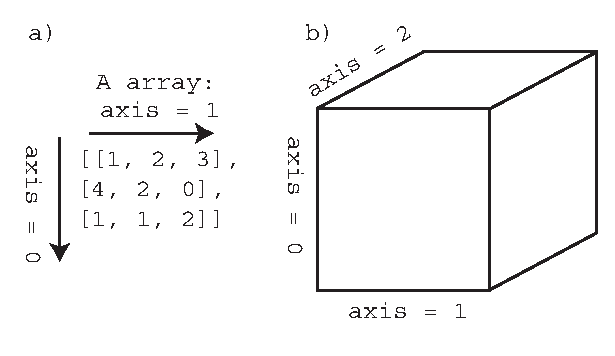
\includegraphics[width=4in]{figures/ndim.eps} 
   
   As shown above our {\color{blue}A} array has two dimensions (axis 0 and 1).  To get Python to tell us this, we use the {\color{blue}ndim} method:
   
   {\singlespacing \color{blue} \begin{verbatim}
>>>  A= numpy.array([[1,2,3],[4,2,0],[1,1,2]]) # just to remind you
>>> A.ndim
2
\end{verbatim}}
Notice how {\color{blue}zeros, ones} and {\color{blue}ndarray} used a shape tuple in order to define the arrays in the examples above.   The shape of an array is how many elements are along each axis.  So, naturally we see that the C array is a 2x3 array.  Python returns a tuple with the shape information using the {\color{blue}shape} method:
{\singlespacing \color{blue} \begin{verbatim}
>>> C.shape
(2, 3)
\end{verbatim}}

Let's say we don't want a 2x3 array for the sequence in the array {\color{blue}C}, but we want a 3x2 array.  Python can reshape an array with a different shape tuple like this:
   {\singlespacing \color{blue} \begin{verbatim}
>>> C.reshape((3,2))
array([[1, 2],
       [3, 4],
       [5, 6]])
\end{verbatim}}

And sometimes we just want all the elements lined up along one axis. We could do that with {\color{blue}reshape} of course using a tuple  with the size of the array (the total number of elements). You  can see that this is 6 here. We could even get python to tell us what the size is ({\color{blue}C.size}) and use that in the reshape size tuple.  Alternatively we can use the {\color{blue}ravel()} method which doesn't require us to know the size in advance:

   {\singlespacing \color{blue} \begin{verbatim}
>>> C.ravel()
array([1, 2, 3, 4, 5, 6])
\end{verbatim}}   

There are other ways to reshape, slice and dice arrays.  
The syntax for slicing of arrays is similar to that for lists:  
{\singlespacing \color{blue} \begin{verbatim}
>>> B=A[0:2] # carve the top two lines off of matrix A from above
array([[1, 2, 3],
       [4, 5, 6]])
\end{verbatim}}

Lots of applications in Earth Science require the transpose of an array:
{\singlespacing \color{blue} \begin{verbatim}
>>> A.transpose() # this is the same as A.T  
array([[1, 4, 7],
       [2, 5, 8],
       [3, 6, 9]])
\end{verbatim}}

Also, we can concatenate two arrays together with the - you guessed it - {\color{blue}concatenate()} method.   For a lot more tricks with arrays, go to the NumPy Reference website here:  http://docs.scipy.org/doc/numpy/reference/.   

 We promised to tell you about matrix objects, so here goes. 
A matrix is another subclass of ndarray with special advantages for particular applications.   
While arrays are intended to be general purpose n-dimensional arrays for numerical computing, 
matrices are better for linear algebra type problems: you can take the inverse and find hermition easier (.I and .H methods) and matrix multiplication works like it does in Matlab for matrix objects, whereas arrays do element-wise computations (we'll learn more about this later).  
Check out this website for more differences between the two: http://www.scipy.org/NumPy\_for\_Matlab\_Users. 



To convert the {\color{blue}A} array to a list:   {\color{blue}L=A.tolist()},  from a list or tuple to an array:   {\color{blue}A=numpy.array(L)}, or from a list, a tuple or an array to a NumPy array:   {\color{blue}a=numpy.asarray(L))}




\section{Python Scripts}

Are you tired of typing yet?  Like UNIX shell scripts, 
Python scripts are programs that can be run and re-run from the command line.
You can type in the same stuff you've been doing interactively into a script file (ending in .py). You can edit scripts with: vi, TextWrangler, Xcode, emacs, etc.  NOT Word!  And then you can run them like this:

{\singlespacing \color{blue} \begin{verbatim}
%python < myscript.py
\end{verbatim}}
 Or you can put in a header line identifying the script as python (\#!/usr/bin/env python), make  it executable (chmod a+x),  and   run it like this:

{\singlespacing \color{blue} \begin{verbatim}
% myscript.py
\end{verbatim}}

Here is a familiar example that creates a script using the UNIX cat command, makes it executable and then runs it:

{\singlespacing \color{blue} \begin{verbatim}
% cat > printmess.py
#!/usr/bin/env python
# simple Python test program (printmess.py)
print 'test message'
^-D
% chmod a+x printmess.py
% ./printmess.py
test message
\end{verbatim}}

\noindent
In a Python script, the  first line MUST be: 

{\singlespacing \color{blue} \begin{verbatim}
#! /usr/bin/env python
\end{verbatim}}

\noindent
so that the file is interpreted as Python.  Unlike Fortran or C, you CANNOT start with a
comment line (try switching lines 1 and 2 and see what happens).

The second line is a comment line.  Anything to the right of \# is assumed to be a comment
(Remember that in Fortran {\color{blue}! } serves the same function).

Notice that print goes by default to your screen.  Because the message is a string, you can use single or double quotes
for the test message.  You can get an apostrophe in your output by using double quotes
and quote marks by using single quotes, i.e.,

{\singlespacing \color{blue} \begin{verbatim}
#! /usr/bin/env python
# simple Python test program 2 (printmess2.py)
print "The pump don't work 'cuz the vandals took the handles"
print 'She said "I know what it\'s like to be dead"'
\end{verbatim}}

\noindent
produces:

{\singlespacing \color{blue} \begin{verbatim}
% ./printmess2.py
The pump don't work 'cuz the vandals took the handles
She said "I know what it's like to be dead"
%
\end{verbatim}}

\noindent
In the second print statement, the $\backslash$' is necessary to prevent an error (try it).   This is an example of a Python `escape code'.   These are used to escape some special meaning, as in an end-quote for a string in this example. We use the backslash to say that we really really want a quote mark here.   Other escape codes are listed here:  

http://www.python-course.eu/variables.php

Here's another example of a program - this one has an typo in line 4:

{\singlespacing \color{blue} \begin{verbatim}
#! /usr/bin/env python
abeg = 2.1
aend = 3.9
adif = aend - abge
print 'adif = ', adif
\end{verbatim}}

\noindent
You had intended to type 'abeg' but typed 'abge' instead.  When
you run the program, you get an error message:

{\singlespacing \color{blue} \begin{verbatim}
Traceback (most recent call last):
  File "./undeclared.py", line 4, in <module>
    adif = aend - abge
NameError: name 'abge' is not defined
\end{verbatim}}

\noindent
Error messages are a desirable feature of Python.  You don't want the program
to run by assigning some arbitrary value to abge and giving you
a wrong answer.  Yet many languages will do exactly that, including
Fortran (we can avoid this potential problem in Fortran by using the 
'implicit none' statement at the beginning our our programs).

\noindent
{\singlespacing \color{red} ASSIGNMENT  P1

  Write a Python script to print your favorite pithy phrase. e-mail your script to ltauxe@ucsd.edu}

\section{A first look at code blocks}
Any reasonable programming language must provide a way to group blocks of code together, to be executed under certain conditions.  In Fortran, for example, there are if statements and do loops which are bounded by the statements if, endif and do, endo respectively.  Many of these programs encourage the use of indentation to make the code more readable, but do not require it.  In Python, indentation is the way that code blocks are defined - there are no terminating statements. Also, the initiating statement terminates in a colon.  The trick is that all code indented the same number of spaces (or tabs) to the right belong together.  The code block terminates when the next line is less indented.     A typical Python program looks like this: 

{\singlespacing \color{blue}\begin {verbatim}
program statement
block 1 top statement:
    block 1 statement
    block 1 statement \
        ha-ha i can break the indentation convention!
    block 1 statement
    block 2 top statement:
        block 2 statement
        block 2 statement
        block 3 top statement:
            block 3 statement
            block 3 statement
            block 4 top statement: block 4 single line of code
        block 2 statement
        block 2 statement
    block 1 statement
    block 1 statement
program statement
\end{verbatim}}


\noindent Exceptions to the code indentation rules are:
\begin{itemize}
\item  Any statement can be continued on the next line with the continuation character $\backslash$ and the indentation of the following line is arbitrary.  \item If a code block consists of a single statement, then that may be placed on the same line as the colon. 
\item The command {\color{blue}break} breaks you out of the code block. Use with caution!
\item There is a cheat that comes in handy when you are writing a complicated program and want to put in the code blocks but don't want them to DO anything yet:  the command  {\color{blue} pass} does nothing and can be used to stand in for a code block.
\end{itemize}

{\singlespacing \color{magenta}Good housekeeping Tip \#2: Always use only spaces or only tabs in your code indentation.  I use only spaces because I use {\color{blue}vi} to write my code.  Others use Xcode, the  Python IDLE program, or TextWrangler to write their code and some of these things use tabs by default.  Whatever you do BE CONSISTENT because tabs are not the same as spaces in Python even if you can't tell the difference just by looking at it.}




In the following, I'll show you how Python uses code blocks  to create ``do'' and ``while'' loops, and ``if'' statements.

\subsection{The for loop}

Here is an example of a ``for loop'' that is similar to the way you would do it in Fortran. :   


{\singlespacing \color{blue} \begin{verbatim}
#!/usr/bin/env python
mylist=[42,`spam',`ocelot']
for i in range(0,len(mylist),1): # note absence of Indices list, start and step
   print mylist[i]
print 'All done' 
\end{verbatim}}

This script creates the list mylist with the line {\color{blue}mylist=[42,`spam',`ocelot']}.  The length of mylist is an integer value returned by {\color{blue}len(mylist)}.      The script uses this integer as the `stop' value in the  {\color{blue}range()} function,  which returns a list of integers from 0 to the stop value  MINUS ONE at intervals of one.   [ The minus one convention is hard to get use to  for Fortran programmers, but it is typical of Python syntax (and also of C) so just deal with it.]  Anyway, {\color{blue}range(start,stop,step)} is just like {\color{blue}numpy.arange(start,stop,step)} but returns integers instead of floats.  Also, like {\color{blue}numpy.arange()}, there is a short hand form when the minimum is zero and the interval is one, so we could (and will)  just use the command {\color{blue}range(stop)}. 
  
   Python makes $i$ step through the list of numbers from 0 to 2, printing the $i^{th}$ element of {\color{blue}mylist}.  Note how the print command is indented - this is the program block that is executed for each $i$.   Note also that the line could have been on the previous line after the colon, because there is only one line in the program block.  But never-mind, this way works too and is more Fortran like.   When $i$ finishes it's business, the program block terminates.   At that point, the program prints out the 'All done' string.   There is no ``enddo'' statement or equivalent in Python.  

But, Python is far more fun than the Fortran-like {\color{blue}for i in} syntax in the above code snippet.  In Python we can just step through a list directly.  Here is another  script which does just that (why not?):  

{\singlespacing \color{blue} \begin{verbatim}
#!/usr/bin/env python
mylist=[42,`spam',`ocelot']
for item in mylist: # note absence of range statement
    print item
print 'All done' 
\end{verbatim}}

\noindent Note that of course we could have used any variable name instead of `item', but it makes sense to use variable names that mean what they do.  It is easier to understand what `item' stands for than just the Fortran style of $i$.  

Here is an example with a little more heft to it.  It creates a table of trigonometry functions, spitting them out with a formatted print statement:

{\singlespacing \color{blue} \begin{verbatim}
#! /usr/bin/env python
import numpy as np
deg2rad = np.pi/180. # remember conversion to radians
for theta in range(90): # short form of range, returns [0,1,2...89]
   ctheta = np.cos(theta*deg2rad) # define ctheta as cosine of theta
   stheta = np.sin(theta*deg2rad)# define stheta as  sine of theta
   ttheta = np.tan(theta*deg2rad)   # define ttheta as tangent of theta
   print '%5.1f %8.4f %8.4f %8.4f' %(theta, ctheta, stheta, ttheta) 
 \end{verbatim}}
 
 Let's pick this one apart a bit.  First, 
notice the use of the variable {\color{blue}deg2rad} to convert from degrees to radians.  Also notice how deg2rad is defined: {\color{blue}deg2rad = np.pi/180.} using the {\color{blue}NumPy} function for $\pi$ and the decimal point after 180.  While in this case, it makes absolutely no difference (try it!), it is a good practice to use real numbers if you want your variable to stay real.  In fact:

{\color{magenta}Good housekeeping Tip \#3:  Always use a decimal if you want your variable to be a floating point variable.}

The expression {\color{blue} ctheta = np.cos(theta*deg2rad)} uses the {\color{blue}numpy} cosine function. Ideally {\color{blue} theta} should be a real variable while in fact it is an integer
  in this expression, but fortunately Python figures that out and converts it to a real.   Note that we could have also converted theta to a float first with the command {\color{blue}float(theta)}.  
  
{\singlespacing \color{blue} \begin{verbatim}  
print '%5.1f %8.4f %8.4f %8.4f' %(theta, ctheta, stheta, ttheta)   
\end{verbatim}}
  
\noindent To make the output look nice, we do not use

{\singlespacing \color{blue} \begin{verbatim}  
print theta, ctheta, stheta, ttheta
\end{verbatim}}

\noindent which would space the numbers irregularly among the columns and put out really long numbers.  Instead,
we explicitly specify the output format.   The output format is given in the quotes.  The format for each
number follows the \%, 5.1f is for 5 spaces of floating point output, with 1
space to the right of the decimal point (in Fortran this is f5.1).  The single
blank space between \%5.1f and \%8.4f is included in the output, in fact any
text there is reproduced exactly in the output, thus to put commas between
the output numbers, write:

{\singlespacing \color{blue} \begin{verbatim}  
print '%5.1f, %8.4f, %8.4f, %8.4f' %(theta, ctheta, stheta, ttheta)   
\end{verbatim}}

\noindent Tabs ($\backslash$t) would be formatted like this:      

{\singlespacing \color{blue} \begin{verbatim}  
print '%5.1f '\t' %8.4f'\t'  %8.4f,\t' %8.4f' %(theta, ctheta, stheta, ttheta) 
\end{verbatim}  }  
  
       
\subsection{If and while blocks}

The ``for loop'' is just one way of controlling flow in Python.  There are also {\color{blue}if}  and  {\color{blue}while} code blocks.  These execute code blocks  the same way as for loops (colon terminated top statements, indented text, etc.).  For both of these, the code block is executed if the top statement is  TRUE.  For the ``if'' block, the code is executed once but in a ``while'' block, the code keeps executing as long as the statement remains TRUE.  

The key to flow control therefore is in the top statement of each code block;  if it is TRUE, then execute, otherwise skip it.  To decide if something is TRUE or not (in the boolean sense), we need to evaluate a statement using comparisons.  You know all about comparisons from Fortran.  Python of course also has comparisons and they work in similar ways with a few differences. Here's a handy table with comparisons (relational operators) in different languages:

\centerline{Comparisons}
\begin{tabular}{cccccl}
\hline
F 77  &   F90    &  C    & MATLAB  & PYTHON  & meaning\\
\hline
.eq.  &  ==   &   ==    &  ==  &     ==   &  equals\\
.ne. &   /=  &    !=   &   $\sim$=    &   !=  &   does not equal\\
.lt.  &  $<$   &    <$<$  &     $<$  &   $<$  &    less than\\
.le.  &  $<$= &     $<$=   &  $<$=   &    $<$=  &   less than or equal to\\
.gt.  & $>$ &      $>$    &   $>$    & $>$   &    greater than\\
.ge.  &  $>$ =   &   $>$ =   &  $>$ =  &    $>$ =  &   greater than or equal to\\
.and. & .and. &   \&&    &  \&  &      and\\
.or.  & .or.  &    ||    &  |   &     or \\ 
\hline
\end{tabular}


These operators can be combined to make complex tests.  Here is a juicy complicated statement:

{\singlespacing \color{blue} \begin{verbatim}
   if ( (a > b and c <= 0) or d == 0):
       code block
   \end{verbatim}}
\noindent   
There are rules for the order of operations for these things like, multiplication gets done before addition.   But these are easy to forget.  You can look it up in the documentation if 
you are unsure or, better, just put in enough parenthesis to 
make it completely clear to anyone reading your code.

\noindent
{\color{magenta}Good housekeeping Tip \#4: Use parentheses liberally - make the order of operation completely unambiguous even if you could get away with fewer. }
  
  
One nice aspect of Python compared to C is that if you make
a mistake and type, for example,

{\color{blue}   \begin{verbatim}
      if (a = 0):
         \end{verbatim}}

\noindent you will get an error message during compilation.  In C this
is a valid statement with a completely different meaning
than is intended!  


\subsubsection{Finer points of `if' blocks}

The simplest `if' block works just like we have described:
{\singlespacing \color{blue} \begin{verbatim}
if (2+2)==4: # note the use of '==' and parentheses in comparison statement
   print `I can put two and two together!'
\end{verbatim}}

However, as in Fortran (and C and any other reasonable programming language), there are whistles and bells to the `if' code blocks.  In Python these are:  {\color{blue}elif} and {\color{blue}else}.  
As in the Fortran equivalent {\color{blue}else if},  the {\color{blue}elif}  code block gets executed if the top {\color{blue}if} statement is FALSE and the  {\color{blue}elif}  statement is TRUE.  If both the top {\color{blue}if} and the {\color{blue}elif}  statements are FALSE but the  {\color{blue}else}  statement is TRUE, then Python will execute the block following the  {\color{blue}else}.  Consider these examples:

{\singlespacing \color{blue} \begin{verbatim}
#!/usr/bin/env python
mylist=['jane','doug','denise']
if 'susie' in mylist:
    pass # don't do anything
if 'susie' not in mylist:
   print 'call susie and apologize!'
   mylist.append('susie')
elif 'george' in mylist: # if first statement is false, try this one
    print 'susie and george both in list' 
else: # if both statements are false, do this:
   print "susie in list but george isn't"
\end{verbatim}}

\subsubsection{While loops}

As already mentioned, the `while' block  continues executing as long as the {\color{blue}while}  top statement is TRUE.  In other words, the if block is only executed once, while the {\color{blue}while}  block keeps looping until the statement turns FALSE.    Here are a few examples:


{\singlespacing \color{blue} \begin{verbatim}
#!/usr/bin/env python
a=1
while a < 10:
    print a
    a+=1
print "I'm done counting!"
\end{verbatim}}

\subsection{Code blocks in interactive Python}

All of these program blocks can also be done in an interactive session also using indentation.  The interactive shell responds with '.....'  instead of '$>>>$' once you type a statement it recognizes as a top statement.   To signal that you are done with the program block, simply hit return: 


{\singlespacing \color{blue} \begin{verbatim}
>>> a=1
>>> while a<10:
....    print a
....    a+=1
....[return to execute block]
\end{verbatim}}



\noindent
{\singlespacing \color{red} ASSIGNMENT  P2

Rewrite your Fortran Assignment F4 in Python. E-mail it to ltauxe@ucsd.edu}




\section{File I/O in Python}

Python would be no better than a rather awkward graphing calculator (and we haven't even gotten to the graphing part yet) if we couldn't read data in and spit data out.   You learned a rudimentary way of spitting stuff out already using the {\color{blue}print} statement, but there is a lot more to file I/O in Python.  We would like to be able to read in a variety of file formats (not just X,Y in the first two columns as in GMT) and output the data any way we want.  In the following we will explore some of the more useful  I/O options in Python.  




\subsection{Reading data in}
\subsubsection{From a file}

If you are using Python interactively or want interactivity in a script,  use the command:  {\color{blue}raw\_input()}.  It acts as a prompt and reads in whatever is supplied prior to a return as a string.  

{\singlespacing \color{blue} \begin{verbatim}
X=[] # make a list to put the data in
ans=float(raw_input("Input numeric value for X:  ")) 
X.append(ans) # append the value to X
print X[-1] # print the last item in the list
\end{verbatim}}
\noindent
In this example, the variable {\color{blue}ans} will be read in as a string variable,  converted to a float and appended to the list, {\color{blue}X}.    {\color{blue}raw\_input()} is a simple but rather annoying way to enter things into a program.  
Another (less annoying)  way is  put the data in a file (e.g., myfile.txt) with cat, paste, Excel (saved as a text file), or whatever and read  it into Python.  The approach to this is similar to Fortran:  we must first open the file, then read it in and parse lines into the desired variables.  

To open a file we use the command {\color{blue}open()}, one of Python's built-in functions.  For a complete list of these, see:

http://docs.python.org/library/functions.html

\noindent  The  {\color{blue}open()} function returns an object,  complete with methods, like {\color{blue}readlines()} which, yes, reads all the lines.  
Here is a script ({\color{blue}ReadStations.py} that will open the file  {\color{blue}station.list} from the chapter on GMT, read in the data and print it out line by line.  
{\singlespacing \color{blue} \begin{verbatim}
#!/usr/bin/env python
f=open('station.list')
StationNFO=f.readlines()
for line  in StationNFO:
    print line
\end{verbatim}}

If you run this script, you will get this behavor:
{\singlespacing \color{blue} \begin{verbatim}
% ReadStations.py
   9.02920   38.76560 2442 AAE 

  42.63900   74.49400 1645 AAK 

  37.93040   58.11890  678 ABKT

  51.88370 -176.68440  116 ADK 
  etc.
  \end{verbatim}}

\noindent The function  {\color{blue}open()} has some bells and whistles to it and has the form  {\color{blue}open(name[, mode[, buffering])} where the stuff in square brackets is optional.  The `name' argument is the file name to open and `mode' is the way in which it should be opened, most commonly for reading 'r', writing 'w' or appending 'a'.  I use the form 'rU' for unformatted reading because I often want to read in files that were saved in Dos, Mac OR Unix line endings and 'rU' figures all that out for you.  Just in case you are curious, Unix lines end in '$\backslash$n',  Mac files in '$\backslash$r' and Dos (and windows) lines end in '$\backslash$r$\backslash$n'.     I never use the 'buffering' argument and don't know what it does.  

If you are curious about the line endings, try typing out the `representation' of the line {\color{blue}repr(line)} in the above script and you get all the  stuff that is normally  invisible like the apostrophes and the line terminations:

{\singlespacing \color{blue} \begin{verbatim}
% ReadStations.py
'   9.02920   38.76560 2442 AAE \n'
'  42.63900   74.49400 1645 AAK \n'
'  37.93040   58.11890  678 ABKT\n'
'  51.88370 -176.68440  116 ADK \n'
' -13.90930 -171.77730  706 AFI \n'
etc.
\end{verbatim}}

  
\noindent Notice how in our first version, printing the line also printed the line feed ($\backslash$n) as an extra line.  To clean this off of each line, we can use the  string {\color{blue}strip()} function:  

{\singlespacing \color{blue} \begin{verbatim}
    print line.strip('\n')
\end{verbatim}}

\noindent Putting this into the code results in this behavior:

{\singlespacing \color{blue} \begin{verbatim}
% ReadStations.py
   9.02920   38.76560 2442 AAE 
  42.63900   74.49400 1645 AAK 
  37.93040   58.11890  678 ABKT
\end{verbatim}}


Let's say you want to read in the data table into lists called Lats, Lons, and StaIDs (the first three columns).  You need to split each line into its columns and append the correct column into the appropriate list.  Fortran automatically splits on the spaces so you probably didn't have to worry about this sort of thing yet, but Python reads in the entire line as a string and ignores the spaces or other possible delimiters (commas, semi-colons, tabs, etc.).  To split the line, we use the string function {\color{blue}split([sep])} where {\color{blue}[sep]} is an optional separator.  If no separator is specified (e.g., {\color{blue}line.split()}), it will split on spaces.   Anything could be a separator, but the most common ones are ',', ';', and '$\backslash$t'.  The latter is how a tab appears if you were to, say, print out the representation of the line, which shows all the invisibles.

Here is a slightly modified version of {\color{blue}ReadStations.py}, {\color{blue}ParseStations.py} which parses out the lines and puts numbers (floats or integers) in the right lists:

{\singlespacing \color{blue} \begin{verbatim}
#!/usr/bin/env python
Lats,Lons,StaIDs,StaName=[],[],[] ,[]# creates lists to put things in
StationNFO=open('station.list').readlines() # combines the open and readlines methods!
for line  in StationNFO:
    nfo=line.strip('\n').split() # strips off the line ending and splits on spaces
    Lats.append(float(nfo[0])) # puts float of 1st column into Lats
    Lons.append(float(nfo[1]))# puts float of 2nd column into Lons
    StaIDs.append(int(nfo[2])) # puts integer of 3rd column into StaIDs
    StaName.append(nfo[3])# puts the ID string into StaName
    print Lats[-1],Lons[-1],StaIDs[-1] # prints out last thing appended
\end{verbatim}}

 \subsubsection{From standard input}

As in Fortran, Python can also read from standard input.  To do this, we need a system specific module, called {\color{blue}sys} which among other things has a {\color{blue}stdin} method.  So, instead of specifying a file name in the {\color{blue}open} command, we could substitute the following line:


{\singlespacing \color{blue} \begin{verbatim}
#!/usr/bin/env python
import sys
Lats,Lons,StaIDs,StaName=[],[],[] ,[]# creates lists to put things in
StationNFO=sys.stdin.readlines() # reads from standard input
for line  in StationNFO:
    nfo=line.strip('\n').split() # strips off the line ending and splits on spaces
    Lats.append(float(nfo[0])) # puts float of 1st column into Lats
    Lons.append(float(nfo[1]))# puts float of 2nd column into Lons
    StaIDs.append(int(nfo[2])) # puts integer of 3rd column into StaIDs
    StaName.append(nfo[3])# puts the ID string into StaName
    print Lats[-1],Lons[-1],StaIDs[-1] # prints out last thing appended
\end{verbatim}}

\noindent The program can be invoked with:

{\color{blue}\begin{verbatim}
% ReadStations.py < station.list
\end{verbatim}}

We could also use command line switches by reading in arguments from the command line.  In the following example, we use the switch '-f' with the following argument begin the file name: 
 
\subsection{Command line switches}

{\singlespacing \color{blue} \begin{verbatim}
#!/usr/bin/env python
import sys
Lats,Lons,StaIDs,StaName=[],[],[] ,[]# creates lists to put things in
if '-f' in sys.argv:  # look in list of command line arguments
    file=sys.argv[sys.argv.index('-f')+1] # find index of '-f' and increment by one
StationNFO=open(file,'rU').readlines() # open file
for line  in StationNFO:
    nfo=line.strip('\n').split() # strips off the line ending and splits on spaces
    Lats.append(float(nfo[0])) # puts float of 1st column into Lats
    Lons.append(float(nfo[1]))# puts float of 2nd column into Lons
    StaIDs.append(int(nfo[2])) # puts integer of 3rd column into StaIDs
    StaName.append(nfo[3])# puts the ID string into StaName
    print Lats[-1],Lons[-1],StaIDs[-1] # prints out last thing appended
\end{verbatim}}

\noindent This version can be invoked with:

{\color{blue}\begin{verbatim}
% ReadStations.py -f  station.list
\end{verbatim}}

\subsubsection{Reading numeric files}

In the special case where the data in a file are entirely numeric, you can read in the file with a special {\color{blue}numpy} function {\color{blue}loadtxt()}.  This reads the data into a list whereby each element of the list is a list of numbers from each line.
 
 \subsection{Writing data out}

Let's say I have a Python module that will convert latitudes and longitudes to UTM coordinates.  O.K. I really do have one that I downloaded from here:  

http://code.google.com/p/pyproj/issues/attachmentText?id=27\&aid=
   
   -80884174771817564 \&name=UTM.py\&token=46ab62caa041c3f240ca0e55b7b25ad6

\noindent I wrote a script ({\color{blue}ConvertStations.py}) to convert each of the stations in my list to their UTM equivalents (assuming these were in a WGS-84 ellipsoid).  It would be nice if  after having done this to the data, I could then write it out somehow, preferably to a file.  Of course I could use the {\color{blue}print} command like this:


 {\singlespacing \color{blue} \begin{verbatim}
#!/usr/bin/env python
import UTM # imports the UTM module
Ellipsoid=23-1 # UTMs code for WGS-84
StationNFO=open('station.list').readlines()
for line  in StationNFO:
    nfo=line.strip('\n').split()
    lat=float(nfo[0])
    lon=float(nfo[1])
    StaName= nfo[3]
    Zone,Easting, Northing=UTM.LLtoUTM(Ellipsoid,lon,lat)
    print StaName, ': ', Easting, Northing, Zone
 \end{verbatim}}

\noindent
which spits out something like this: 

{\singlespacing \color{blue} \begin{verbatim}
% ConvertStations.py
AAE :  474238.170087 998088.469113 37P
AAK :  458516.115522 4720850.45385 43T
ABKT :  598330.712671 4198681.92944 40S
ADK :  521722.179764 5748148.625 1U
AFI :  416023.683618 8462168.07766 2L
etc.
\end{verbatim}}

\noindent 
I could save the output with a UNIX re-direct: 
 {\singlespacing \color{blue} \begin{verbatim}
ConvertStations.py > mynewfile
 \end{verbatim}}
 
But we yearn for more.  So,  more  elegantly, I can open an output file [for appending `a' or (over)writing 'w']  write a formatted string using the write method on  the output file object with format string:

 {\singlespacing \color{blue} \begin{verbatim}
#!/usr/bin/env python
import UTM # imports the UTM module
outfile=open('mynewfile','w') # creates outfile object
Ellipsoid=23-1 # UTMs code for WGS-84
StationNFO=open('station.list').readlines()
for line  in StationNFO:
    nfo=line.strip('\n').split()
    lat=float(nfo[0])
    lon=float(nfo[1])
    StaName= nfo[3]
    Zone,Easting, Northing=UTM.LLtoUTM(Ellipsoid,lon,lat)
    outfile.write('%s  %s  %s  %s\n'%(StaName, Easting, Northing, Zone))
\end{verbatim}}

\noindent
The only significant changes are 1) the object {\color{blue}outfile} is opened for writing. Note that this will clobber anything in a pre-existing file by that name and 2) the output file gets written to in the statement with a write method on the output file object:
{\singlespacing \color{blue} \begin{verbatim}
    outfile.write('%s  %s  %s  %s\n'%(StaName, Easting, Northing, Zone))
\end{verbatim}}
\noindent
The write statement uses the syntax:  'format string'\%(list of variables tuple).  Format strings have these rules:

\begin{itemize}
\item For each variable in (what you...) you need a format:  \%s for string, \%i for integer, \%f for float, \%e for exponent
\item you can also specify further, e.g.:
\%7.1f  for 7 characters with 1 after the decimal
\%10.3e for 10 characters with 3 after the decimal
\item where the number of characters include the decimal and padded spaces
\item As noted before, the format string can include punctuation:
\end{itemize}
{\singlespacing \color{blue} \begin{verbatim}
x,y=4.82,2.3e3
print '%7.1f,%s\t%10.3e'%(x,'hi there',y)
   4.8,hi there	 2.300e+03
\end{verbatim}}
\begin{itemize}
\item In the {\color{blue}ConvertStations2.py} script, the  '$\backslash$n' string puts a UNIX line ending on it.  Without that, the whole file is but a single line (very annoying).  
\end{itemize}




\noindent A session using the script ({\color{blue}ConvertStations2.py} and a peek at the resulting file could look like this:
{\singlespacing \color{blue} \begin{verbatim}
% ConvertStations2.py
% head mynewfile 
AAE  474238.170087  998088.469113  37P
AAK  458516.115522  4720850.45385  43T
ABKT  598330.712671  4198681.92944  40S
ADK  521722.179764  5748148.625  1U
AFI  416023.683618  8462168.07766  2L
ALE  509467.666259  9161062.29194  20X
ALQ  366981.843985  3868044.56906  13S
ANMO  366981.843985  3868044.56906  13S
ANTO  482347.254856  4413225.7807  36S
AQU  368638.770654  4690300.1797  33T
\end{verbatim}}

\noindent  I'm assuming you know what the UNIX {\color{blue}head} command does or at least how to find out! 


\section{Functions}

So far you have learned how to use functions from program modules like {\color{blue}NumPy}.  You can imagine that there are many bits of code that you might write that you will want to use again and again, say converting between degrees and radians and back, or finding the great circle distance between two points on Earth, or converting between UTM and latitude/longitude coordinates (as in {\color{blue}UTM.py}, my new favorite package).   In Fortran, you learned about subroutines and functions which do this sort of work for you.  In Python, we also have a way to do this of course.    The basic structure of a program with a  Python function is: 


{\singlespacing \color{blue} \begin{verbatim}
#!/usr/bin/env python

def FUNCNAME(in_args):  
    """
    DOC STRING
    """
    some code that the functions does something
    return out_args
    
FUNCNAME(in_args) # this calls the function
\end{verbatim}}



\subsection{Line by line analysis}
\subsubsection{def FUNCNAME(in\_args):}

\noindent The first line must have 'def' as the first three letters, must have a function name with parentheses and a terminal colon.  If you want to pass some variables to the function, they go where  in\_arg sits, separated by commas.  Unlike in Fortran, there are no output variables here.  

 There are four different ways to handle argument passing. 
 
 1) You could have a function that doesn't  need any arguments at all:
 
 {\singlespacing \color{blue} \begin{verbatim}
 #!/usr/bin/env python
def gimmepi():  
    """
    returns pi
    """
    return 3.141592653589793
print gimmepi()
\end{verbatim}}

\noindent 2)  You could use a Fortran like style, where there is a set list of what are called `formal' variables that must be passed:  
 

{\singlespacing \color{blue} \begin{verbatim}
#!/usr/bin/env python
def deg2rad(degrees):  
    """
    converts degrees to radians
    """
    return degrees*3.141592653589793/180.
print '42 degrees in radians is: ',deg2rad(42.)
\end{verbatim}}
    
\noindent 3) You could have a more flexible need for variables.  You signal this by putting  *args in the in\_args list (along with any formal variables you want):

{\singlespacing \color{blue} \begin{verbatim}
#!/usr/bin/env python
def print_args(*args):
    """
    prints argument list
    """
    print 'You sent me these arguments: '
    for arg in args:
        print arg
print_args(1,4,'hi there')
print_args(42)
\end{verbatim}}

\noindent 4) You can use a keyworded, variable-length list by putting **kwargs in for in\_args:

{\singlespacing \color{blue} \begin{verbatim}
#!/usr/bin/env python
def print_kwargs(**kwargs):
    """
    prints keyworded argument list
    """
    for key in kwargs:
        print '%s  %s' %(key, kwargs[key])
     
print_kwargs(arg1='one',arg2=42,arg3='ocelot')
\end{verbatim}}

 \subsubsection{Doc String}
 Although you can certainly write functional code without a document string, make a habit of always including one.  Trust me - you'll be glad you did.  This can later be used to remind you of what you thought you were doing years later.  It can be used to print out a help message by the calling program and it also let's others know what you intended.   Notice the use of the triple quotes before and after the documentation string - that means that you can write as many lines as you want.  
 
 \subsubsection{Function body}
 This part of the code must be indented, just like in a for loop, or other block of code.  
 
 \subsubsection{Return statement}
 You don't need this unless you want to pass back information to the calling body (see, for example {\color{blue}print\_kwargs()} above).  But unlike in Fortran, where variables are passed back the same way they get in, through the first line, Python separates the entrance and the exit.  See how it can be done in the {\color{blue}gimme\_pi()} example above.    
 
 \subsection{Main program as function}
 
 It is considered good Python style to treat your main program block as a function too.  (This helps with using the document string as a help function and building program documentation in general.)  In any case, I recommend that you just start doing it that way too.  In this case,  we have to call the main program with the final (not indented) line {\color{blue}main()}:

{\singlespacing \color{blue} \begin{verbatim}
#!/usr/bin/env python
def print_kwargs(**kwargs):
    """
    prints keyworded argument list
    """
    for key in kwargs:
        print '%s  %s' %(key, kwargs[key])
     
def main():
    """
    calls function print_kwargs
    """
    print_kwargs(arg1='one',arg2=42,arg3='ocelot')
main()  # runs the main program
\end{verbatim}}

Notice how in the above examples, all the functions preceded the main function.  This is because Python is an interpreter and not compiled - so it won't know about anything declared below as it goes through the script line by line.   On the other hand, we've been running lots of functions and they were not in the program we used to call them.  The trick here is that 
you can put a bunch of functions in a separate file (in your path) and import it, just like we did with {\color{blue}NumPy}.  Your functions can then be called from within your program  in the same way as for {\color{blue}NumPy}.  

So let's say I put all the above functions in a file called {\color{blue}myfuncs.py}:

{\singlespacing \color{blue} \begin{verbatim}
def gimmepi():  
    """
    returns pi
    """
    return 3.141592653589793
def deg2rad(degrees):  
    """
    converts degrees to radians
    """
    return degrees*3.141592653589793/180.
def print_args(*args):
    """
    prints argument list
    """
    print 'You sent me these arguments: '
    for arg in args:
        print arg
\end{verbatim}}

\noindent I could then just import the module {\color{blue}myfuncs} from within another program, or just interactively.  I can use the functions, or just call for help:

{\singlespacing \color{blue} \begin{verbatim}
% python
>>> import myfuncs
>>> print myfuncs.gimmepi()
3.14159265359
>>> print myfuncs.print_args.__doc__

    prints argument list

>>>
\end{verbatim}}

\subsection{Scope of variables}

As in Fortran, inside a function,  variable names have their own meaning  which in many cases will be different from inside the calling function.  So,  variables names declared inside a function stay in the function.  This is true unless you declare them to be ``global''.
Here is an example in which the main program  ``knows'' about the functions variable {\color{blue}V}:  

{\singlespacing \color{blue} \begin{verbatim}
def myfunc():
    global V
    V=123
def main():
    myfunc()
    print V
main()
\end{verbatim}}







In addition to being able to write your own functions, of course 
Python has LOTS of modules and a gazzillion functions. The enthought distribution that you are using
Includes plotting, numerical recipes, trig functions, image manipulation, animation,  and many more. We will explore some of these in the rest of the class.  


\noindent
{\color{red}ASSIGNMENT P3:    

\singlespacing 
Write a subroutine module that has these functions:
\begin{itemize}
\item a function that returns the bulk parameters relating to the Earth from this website: 

http://nssdc.gsfc.nasa.gov/planetary/factsheet/earthfact.html

Also include the average radius of: 6,371 km
\item a function that converts degrees to radians
\item one that converts radians to degrees
\item one that converts longitude and latitude to cartesian coordinates. [hint, $x=\cos(az)\cos(pl),y=\sin(az)\cos(pl),z=\sin(pl)]$], assuming a radius of unity
\item one that converts cartesian coordinates back to longitude and latitude
\item and one that calculates the great circle distance between two points using the {\color{blue}numpy.dot()} function  to get the angular separation and the radius of the Earth to get the arc length.   Assume the average radius of the Earth (gotten from the first function).
\end{itemize}
Then write a  program that takes keyboard entry for an longitude and latitude pair and prints out the X,Y,Z,  
converts back and prints the new longitude and latitude out (as a check) and gives you the great circle distance in km. [HINT: Take a look at the function {\color{blue}SPH\_AZI} in the Fortran chapter.]
E-mail your code to ltauxe@ucsd.edu}


\section{Combining F90 code with Python}

Now you have the very basics of Python programming under your belt, we can try to pull together the different threads you have been learning by investigation how to combine F90 with Python.  You might ask why not just use Python?  or Fortran?  The answer is that there is a lot of Fortran code lying around that you might want to use, but no way to visualize the data, so you want Python for that.  Or you are solving an extremely computationally intensive problem (global climate model, or convection in the Earth's core or mantle, or ....) and you need code that is  as fast as possible. Although {\color{blue}NumPy} is compiled and therefore very fast,  Fortran is still the fastest thing around.  For whatever reason, you are taking a class in both Fortran and Python so it makes pedagogical sense to try to tie the two halves together.  

The next question is ``How?''.  There are several different approaches to this ranging from the simple to the sophisticated.  The simple approach would be to create output files with Fortran and the read it in and plot it or whatever with Python.  A more sophisticated approach would be to call subroutines and functions from a Fortran module which is imported like any other module into Python.   This is more tricky and involves a Python package called {\color{blue}f2py} which came with your Python distribution.  



I have tested {\color{blue}f2py}   using the gfortran and python packages that were recommended for this class and it worked fine.  But I  also had  to get rid of  my beloved antique /usr/local/bin/g77 compiler, but you probably don't have one.  This is just a trouble shooting tip.  For reference, the URLs for these are:

http://gcc.gnu.org/wiki/GFortranBinaries\#MacOS

\noindent
and 

http://www.enthought.com/products/getepd.php

\noindent Because these websites change quickly, I also put the .dmg files on the class website:

http://mahi.ucsd.edu/class233/gfortran-and-gcc-4-6-2-RC20111019-Sno-x86-64.dmb
\noindent

and

http://mahi.ucsd.edu/class233/epd-7.1-2-macosx-i386.dmb




Assuming you have installed everything properly, there we will cover three ways to use {\color{blue}f2py} in the following.  These are:


\begin {itemize}
\item Brute force:  Try to get  {\color{blue}f2py} to create a compiled module (ending in .so) from a standard F90 program, which can then be imported like any other module. Because Fortran subroutines have arguments that both go into the subroutine and come out,  and Python doesn't, {\color{blue}f2py} has to make guesses as to the use of  variables and does its best.  This works in simple cases, but can fail badly at times. 
\item Signature File:  Ask {\color{blue}f2py} to read through the code, picking out all the variables and create what is called a ``signature file'' (ending in .pyf).  This has {\color{blue}f2py}'s guesses as to what the variables are supposed to do.  The signature file  can be edited to supply the correct intent of variables. Then {\color{blue}f2py} can create the compiled module based on what is in the signature file, which functions with fewer errors (from bad guesses).  
\item F90 surgery:  The Fortran code can be modified itself to help {\color{blue}f2py} in interpreting variables.
\end{itemize}


\subsection{Brute force {\color{blue}f2py} method:}

Let's start with an example using  the program {\color{blue}gcf2.f90}  from the chapter on Fortran.  This  has a function to calculate greatest common factors.  In fact we don't need all the fiddly bits at the top - just the function {\color{blue}getgcf}.  Let's save it  in a file called {\color{blue}gcf.f90}:


{\singlespacing \color{blue} \begin{verbatim}
function getgcf(x, y) 
   implicit none
   integer :: getgcf, x, y, i, z
   do i = 1, min(x,y)
      if (mod(x, i) == 0 .and. mod(y, i) == 0) getgcf = i
   end do
end function getgcf
\end{verbatim}}

To compile the function (or the whole program!),  use this syntax:

{\singlespacing \color{blue} \begin{verbatim}
f2py -c gcf.f90 -m gcf
\end{verbatim}}

\noindent The {\color{blue}-c} switch specifies which file to compile and the {\color{blue}-m} switch specifies the stem of the output file.  {\color{blue}f2py} will create something called that stem with  {\color{blue}.so} appended to it, so if all is well you will get a file called {\color{blue}gcf.so}.  
The output file {\color{blue}gcf.so}  is a callable module from within python:

{\singlespacing \color{blue} \begin{verbatim}
>>> import gcf  # note that no .so is needed
>>> gcf.getgcf(8,4) # call the function in the usual way
4
\end{verbatim}}


The brute force method is not without potential problems.  For example, we could use the function without checking for variable type and send the F90 function something with  the wrong type,  getting back the wrong answer with no error message. Also, {\color{blue}f2py}  assumes that all variables are going IN to the subroutine and doesn't know that some are intended to come out.  
 So we need a way to ``teach'' {\color{blue}f2py}  which variables are intended to go in and which are intended to come out.
This can be done either with a ``signature file'' if you can't modify the Fortran code itself, or by inserting a few python hints into the Fortran code itself.

To illustrate the problem, let's consider  another F90 subroutine {\color{blue}sph\_azi} from the Fortran chapter:


{\singlespacing \color{blue} \begin{verbatim}
subroutine SPH_AZI(flat1, flon1, flat2, flon2, del, azi)
   implicit none
   real :: flat1,flon1,flat2,flon2,del,azi,pi,raddeg,theta1,theta2,  &
           phi1,phi2,stheta1,stheta2,ctheta1,ctheta2,                &
           sang,cang,ang,caz,saz,az
   if ( (flat1 == flat2 .and. flon1 == flon2) .or.     &
        (flat1 ==  90.  .and. flat2 ==  90.)  .or.     &
        (flat1 == -90.  .and. flat2 == -90.) )  then
      del=0.
      azi=0.
      return
   end if
   pi=3.141592654
   raddeg=pi/180.
   theta1=(90.-flat1)*raddeg
   theta2=(90.-flat2)*raddeg
   phi1=flon1*raddeg
   phi2=flon2*raddeg
   stheta1=sin(theta1)
   stheta2=sin(theta2)
   ctheta1=cos(theta1)
   ctheta2=cos(theta2)
   cang=stheta1*stheta2*cos(phi2-phi1)+ctheta1*ctheta2
   ang=acos(cang)
   del=ang/raddeg
   sang=sqrt(1.-cang*cang)
   caz=(ctheta2-ctheta1*cang)/(sang*stheta1)
   saz=-stheta2*sin(phi1-phi2)/sang
   az=atan2(saz,caz)
   azi=az/raddeg
   if (azi.lt.0.) azi=azi+360.
end subroutine SPH_AZI
\end{verbatim}}

 
\noindent
 
Let's  try the brute force  {\color{blue}f2py} way:

{\singlespacing \color{blue} \begin{verbatim}
f2py -c sph_azi.f90 -m sph_azi
\end{verbatim}}

\noindent
and try {\color{blue} sph\_azi} out in Python:

{\singlespacing \color{blue} \begin{verbatim}
%python
>>> import sph_azi
>>> delta,azi=0.,0. # have to declare these..
>>> sph_azi.sph_azi(33,-117,41,-72,delta,azi) # note module/function name are same.
>>> print delta, azi
0.0 0.0
\end{verbatim}}



Well, that didn't work.  The problem is that   Python can't get the variables {\it delta, azi} back out from the subroutine.  The Fortran style of using the entrance as the exit makes it tough to figure out which variables are supposed to go in and which are supposed to come out, to {\color{blue}f2py} doesn't even try.  The solution is to use the ``signature file'' method. 

\subsection{Signature files}

We can use {\color{blue}f2py} to create a signature file {\color{blue} sph\_azi.pyf} with the command: 


{\singlespacing \color{blue} \begin{verbatim}
f2py sph_azi.f90 -m sph_azi -h sph_azi.pyf
\end{verbatim}}

\noindent The syntax is a little different  from the brute force method in that we are not compiling {\color{blue}sph\_azi} yet, we are just creating the .pyf file (specified by the {\color{blue}-h} switch, for use in the eventual {\color{blue}sph\_azi} module (specified by the {\color{blue}-m} switch).  

If we look inside the {\color{blue}ph\_azi.pyf} file, we find:


{\singlespacing \color{blue} \begin{verbatim}
!    -*- f90 -*-
! Note: the context of this file is case sensitive.

python module sph_azi ! in 
    interface  ! in :sph_azi
        subroutine sph_azi(flat1,flon1,flat2,flon2,del,azi) ! in :sph_azi:sph_azi.f90
            real :: flat1
            real :: flon1
            real :: flat2
            real :: flon2
            real :: del
            real :: azi
        end subroutine sph_azi
    end interface 
end python module sph_azi

! This file was auto-generated with f2py (version:2).
! See http://cens.ioc.ee/projects/f2py2e/
\end{verbatim}}


\noindent  At this point, all we have is a list of  all the variables {\color{blue}f2py} found.  Note that while Fortran doesn't care about case, Python does, so the variable names within the .f90 code are converted to lower case by default.  (You can suppress this with the {\color{blue}--n-lower} switch.)
The default assumption is that all of the variables found are headed IN to the subroutine and not intended to come out. 
Because in the case of {\color{blue}sph\_azi} this is not true ({\color{blue}del} and {\color{blue}azi} are coming out),  we must edit the .pyf file to explicitly say which variables are coming in and which are coming out. This is done with the by inserted the function {\color{blue}intent(in)} or {\color{blue}intent(out)} after the variable type:  

{\singlespacing \color{blue} \begin{verbatim}
python module sph_azi ! in 
    interface  ! in :sph_azi
        subroutine sph_azi(flat1,flon1,flat2,flon2,del,azi)
            real intent(in) :: flat1
            real intent(in):: flon1
            real intent(in):: flat2
            real intent(in) :: flon2
            real intent(out) :: del
            real intent(out) :: azi
        end subroutine sph_azi
    end interface 
end python module sph_azi
\end{verbatim}}


\noindent If we save the modified .pyf file as {\color{blue}sph\_azi1.pyf}, we can compile {\color{blue}sph\_azi}   with the command:

{\singlespacing \color{blue} \begin{verbatim}
% f2py -c sph_azi1.pyf sph_azi.f90
\end{verbatim}}

\noindent which creates a new file {\color{blue}sph\_azi.so}.  Let's see if that one works better: 

{\singlespacing \color{blue} \begin{verbatim}
% python
>>> import sph_azi
>>> delta,azi=sph_azi.sph_azi(33,-117,41,-72)
>>> print delta, azi
36.4012794495 64.0623321533
\end{verbatim}}

\noindent And it does!   

\subsection{F90 Surgery}

In the last section we saw how to use F90 code, without touching it, just by clarifying a few things for poor old {\color{blue}f2py}.  
 IF you can modify the F90 source, you can skip the signature file by inserting special commands, called `f2py directives'   that the Fortran compiler will ignore (because they start with a '!'), but f2py will recognize (sneaky, huh?).  Here is an example of a duly  modified code, saved as {\color{blue}sph\_azi2.f90}:


{\singlespacing \color{blue} \begin{verbatim}
subroutine SPH_AZI(flat1, flon1, flat2, flon2, del, azi)
   implicit none
   real :: flat1,flon1,flat2,flon2,del,azi,pi,raddeg,theta1,theta2, &
           phi1,phi2,stheta1,stheta2,ctheta1,ctheta2,   &
           sang,cang,ang,caz,saz,az
!f2py intent(in) flat1
!f2py intent(in) flon1
!f2py intent(in) flat2
!f2py intent(in) flon2
!f2py intent(out) del
!f2py intent(out) azi
   if ( (flat1 == flat2 .and. flon1 == flon2) .or.     &
        (flat1 ==  90.  .and. flat2 ==  90.)  .or.     &
        (flat1 == -90.  .and. flat2 == -90.) )  then
      del=0.
      azi=0.
      return
   end if
   pi=3.141592654
etc.
\end{verbatim}}

\noindent  We can then compile the modified code with the command:

{\singlespacing \color{blue} \begin{verbatim}
f2py -c -m sph_azi2 sph_azi2.f90
\end{verbatim}}

This works just like the signature file example but using the module name {\color{blue}sph\_azi2} instead of {\color{blue}sph\_azi}.    


\subsection{A few more things you need to know:}

\begin{itemize}
\item NB: If you are modifying Fortran 77, then use  {\color{blue}Cf2py} instead of `{\color{blue}f2py}' but this isn't included in the Enthought Python you installed, and I have never used it, so you are on your own here.
\item For variables that are both in and out, use:  intent(inout)
\item For variables are are change in place, use:  intent(inplace)
\item For allocatable variables, use, e.g., intent(out,allocatable)
\item Watch out with arrays -- Fortran and the default {\color{blue}NumPy} arrays are the transpose of one another!   There are ways spelled out in the {\color{blue}NumPy} documentation for making your Pytnon arrays behave the same as the Fortran ones - so go read that before you get fancy ideas.
\item {\color{blue}f2py} converts all the Fortran subroutine names to lower case.  You can suppress this with a --n-lower option.  
\item For more detailed information on what {\color{blue}f2py}  is really doing, see the documentation available here:
\end{itemize}

http://www.scipy.org/F2py

\noindent
There is also a helpful, but somewhat dated reference manual available here:

http://cens.ioc.ee/projects/f2py2e/usersguide/

\noindent Note that in the latter, there are many references to a module named {\color{blue}Numeric}, which is a predecessor of {\color{blue}NumPy} - so don't try to call it because you don't have it installed. 



\noindent
{\singlespacing \color{red} ASSIGNMENT  P4

Modify your ASSIGNMENT F8 such that that main program is in Python and calls your  F90 subroutine.  Use the F90 surgery method above to modify your subroutine such that it compiles without the use of signature files.  E-mail both files plus the script you would use to compile them to ltauxe@ucsd.edu
}

\section{Classes}

Before we go any further, we need to learn some basic concepts about classes. These 
 are the basis of  ``object oriented programming'' OOP (that again!).   Class objects lie behind plotting, for example and a rudimentary understanding of what they are and how they work will come in handy when we start doing anything but the simplest plotting exercises.  
 
  A class object is   created by a call  to a ``class definition''  which which can be thought of as a blueprint for the class object.  Here is an simple example of a class definition:

{\singlespacing \color{blue} \begin{verbatim}
class Circle:
    """
    This is simple example of a class
    """
    pi=3.141592653589793
    def __init__(self,r):
        self.r=r
    def area(self):
        return 0.5*self.pi*self.r**2
    def circumference(self):
        return 2.*pi*self.r

\end{verbatim}}

\noindent Saving this class in a file called {\color{blue}Shapes.py} we can use it in a Python session in a manner similar to function modules:

{\singlespacing \color{blue} \begin{verbatim}
>>> import Shapes # import the class
>>> r=4.0
>>> C=Shapes.Circle(r) # create a class instance with r=4.
>>> C.pi  # retrieve an attribute
3.141592653589793
>>> C.area() # retrieve a method
25.132741228718345
>>> C.r=2.0 # change the value of r
>>> C.area() # get a new area
6.283185307179586
\end{verbatim}}

\noindent In spite of superficial similarities, classes are not the same as functions.  Although the Shape module is imported just the same as any other, to use it, we first have to create a class ``instance'' ({\color{blue}C=Shapes.Circle(r)}).  {\color{blue}C} is an object with 	``attributes'' (variables) and ``methods''.  
All methods (parts that start with ``def''),  have an argument list. The first argument has to be a reference to the class instance itself, or ``self'', followed by any variables you want to pass into the method.  So the {\color{blue}\_\_init\_\_} method initializes the instance attributes of an object.  In the above case, it defined the attribute {\color{blue}r}, which gets passed in when the class is first called.  
Asking for any attribute (note the lack of parentheses), retrieves the current value of that attribute.  Attributes can be changed (as in  {\color{blue}C.r=2.0}).   

The other methods ({\color{blue}area} and {\color{blue}circumference}) are defined like any function except note the use of 'self' as the first argument.  This is required in all class method definitions.  In our case, no other parameters are passed in because the only one used is {\color{blue}r}, so the argument list consists of only {\color{blue}self}.  Calling these methods returns the current values of these methods.   

You can make a subclass (child) of the parent class which has all the attributes and methods of the parent, but may have a few attributes and methods of its own.   You do this by setting up another class definition within a class.  

So, the bottom line about classes is that they are  in the same category of things as variables, lists, dictionaries, etc. That is, they are  `data structures' - they hold data, and the methods to process that data.
If you are curious about classes, there's lots more to know about classes that we don't have time to get into, but you can find useful tutorials online:

 (e.g., http://www.sthurlow.com/python/lesson08/)
 
\noindent
{\singlespacing \color{red} ASSIGNMENT  P5
\begin{itemize}
\item Write a module called Shapes
\item Shapes should have classes for:  circle, sphere, cylinder, rectangle, and cube.
\item these classes should have methods that return things volume, circumference, area, mass (pass the argument density), where appropriate.  
\item write a class called Earth that has attributes using the bulk parameters from assignment P3
\item write a program that uses the Earth density, radius from the Earth class, passes these to the sphere class and calculates the mass.  How does this compare with the mass given by the Earth class?  
\end{itemize}
}



\section{Matplotlib}

So far you have learned the basics of Python, NumPy and how to link F90 code with Python.  But Python was sold as a way of visualizing data and we haven't yet seen a single plot!  There are many plotting options within the Python umbrella. The most mature and the one I am most familiar with is {\color{blue}matplotlib}, a popular  graphics module of Python.  
Actually  {\color{blue}matplotlib} is a collection of a bunch of other modules, toolkits, methods and  classes.   For a fairly complete and readable tour of matplotlib, check out these links:  
 
http://matplotlib.sourceforge.net/Matplotlib.pdf

\noindent
and here:

http://matplotlib.sourceforge.net/




\subsection{A first plot}

Let's start with a simple plot script ({\color{blue}matplotlib1.py}):


{\singlespacing \color{blue} \begin{verbatim}
#!/usr/bin/env python
import matplotlib
matplotlib.use("TkAgg") # my favorite backend
import pylab # module with matplotlib
pylab.plot([1,2,3])  # plot some numbers
pylab.ylabel('Y') # label the y-axis
pylab.show() # reveal the plot
\end{verbatim}}



The first step should be obvious by now, it imports {\color{blue}matplotlib}.
Figures are rendered on ``backends'' so they appear on screen.  There are a lot of different back-ends with slightly different looks.  Some work better on different operating systems.  I use the very old school backend called  ``TkAgg'' backend because it ``works''.  So step 2  sets the backend: {\color{blue}matplotlib.use(``TkAgg'')}.  The module {\color{blue}matplotlib} itself contains a lot of other modules.  One of these, 
{\color{blue}pylab} is the ``business end'' that has a lot of plotting methods and classes.  It must be  loaded alongside {\color{blue}matplotlib},   so step 3 is:  {\color{blue}import pylab}. After that the fun starts.  

In the above example, we call the {\color{blue}plot} method with a list as an argument.  As I mentioned, {\color{blue}matplotlib} uses the concept of ``classes'' to make plots and this has just happened behind the scenes. We could have named the plot instance with a the {\color{blue}figure()} method (e.g.,  {\color{blue}fig=pylab.figure()}) and then referred to it later with the command  {\color{blue}fig.plot([1,2,3])}, but we don't have to in this simple case - the class instance is implied and is the ``current plot''.  You can tell this, if you do the above example in interactive mode:

{\singlespacing \color{blue}\begin{verbatim}
>>> import matplotlib
>>> matplotlib.use("TkAgg")
>>> import pylab
>>> pylab.plot([1,2,3])
[<matplotlib.lines.Line2D object at 0x4bd6eb0>]
\end{verbatim}}
\noindent The bit about {\color{blue}[$<$matplotlib.lines.Line2D object at 0x4bd6eb0$>$]} is Python's way of telling you that you just created an object and something about it.   
In any case, when you give {\color{blue} plot()} a single sequence of values (as above), it assumes they are $y$ values and supplies the $x$ values for you.  

Attributes of the {\color{blue}pylab} class, such as the Y axis label can be changes with the {\color{blue}ylabel} method.  As you can imagine, there are LOTS of methods, including, surprise, an {\color{blue}xlabel} method.  

When we are done customizing the plot instance, we can view it with the {\color{blue}show} method.  When that gets executed, we will get a plot something like this:

   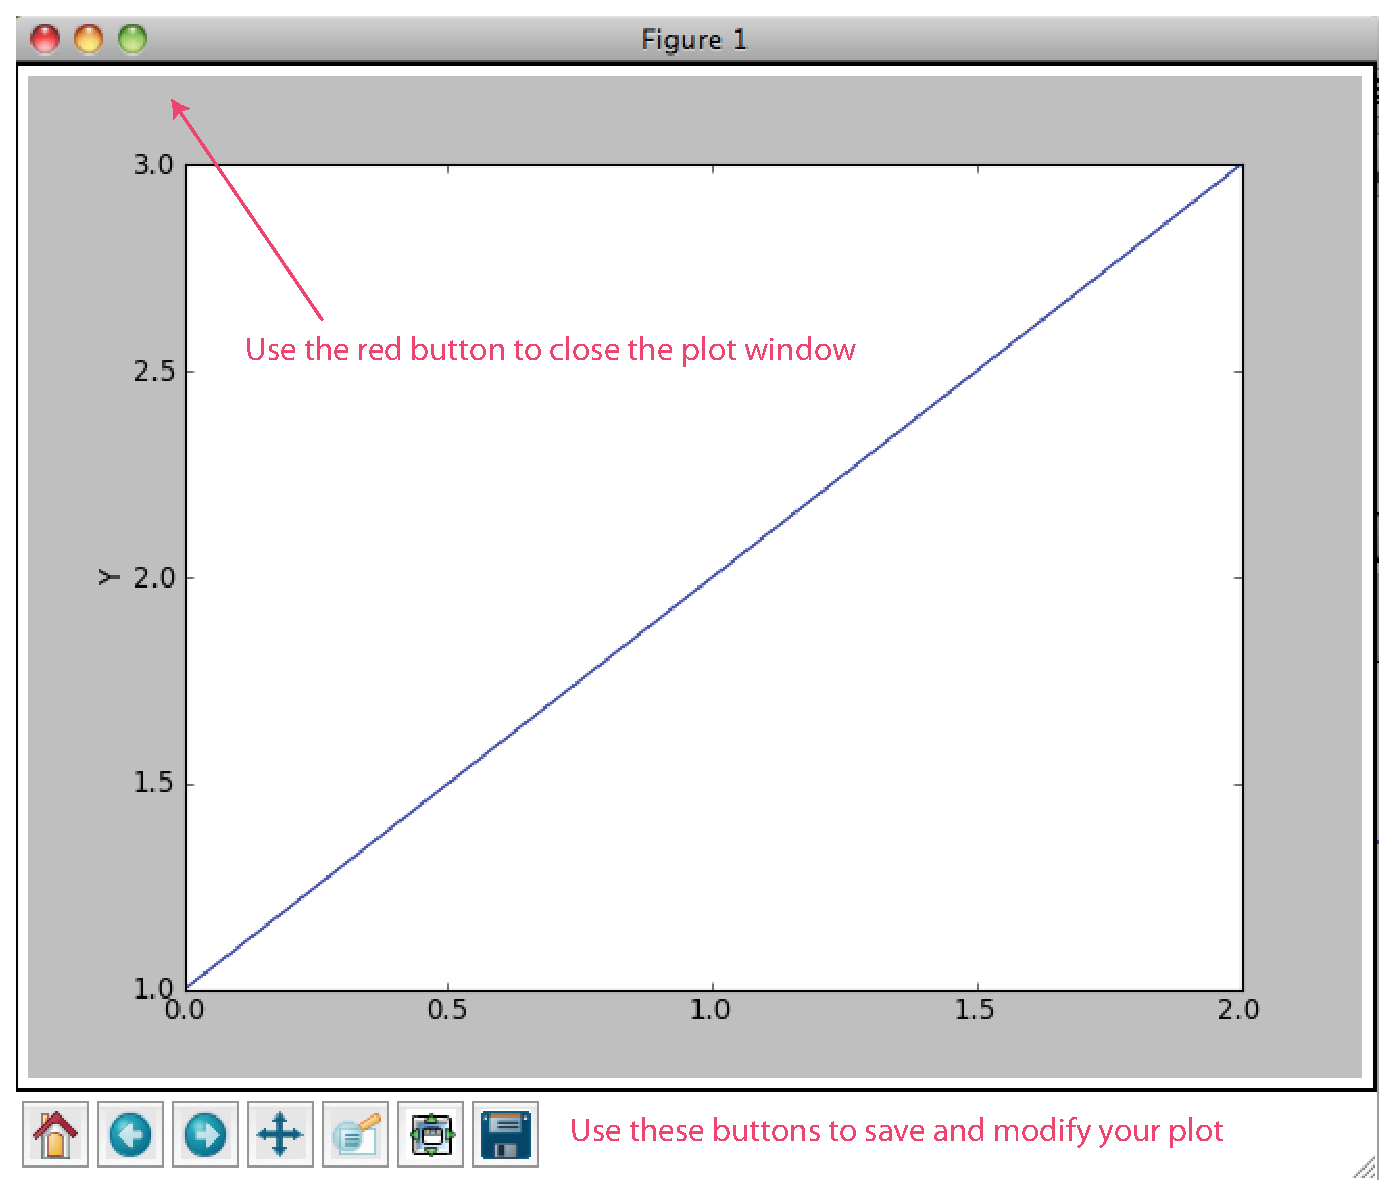
\includegraphics[width=5in]{figures/matplotlib1.eps} 
   
   \noindent Once that happens, we won't be able to change the plot any more and in fact, we won't get our terminal back until the little plot window is closed.   You can save your plot with the little disk icon in a variety of formats.  Adobe Illustrator likes .svg, or .eps while Microsoft products like .png file formats.  

If you find it annoying to always have to close figures with the little red button, or save them with the disk icon, you can tweak the program like this:

{\singlespacing \color{blue}\begin{verbatim}
#!/usr/bin/env python
import matplotlib
matplotlib.use("TkAgg") 
import pylab 
pylab.ion()  # turn on interactivity
pylab.plot([1,2,3]) 
pylab.ylabel('Y') 
pylab.draw() # draw  the current plot
ans=raw_input('press [s] to save figure, any other key to quit: ')
if ans=='s':
    pylab.savefig('myfig.eps')
\end{verbatim}}

\noindent The method {\color{blue}pylab.savefig(FILENAME.FMT)}.  The .FMT can be one of several, e.g., .eps, .svg, .ps, .pdf, .png, .gif, .jpg, etc.).   Some of these (the vector graphics ones like pdf,  ps, eps and svg) can be opened in Adobe Illustrator for modification.   


As mentioned earlier, if  you give {\color{blue}plot()} a single sequence of values, it assumes they are $y$ values and supplies the $x$ values for you.  Garbage in, garbage out.  But 
 {\color{blue}plot()} takes an arbitrary number of arguments of the form: ($X_1, Y_1$, line\_style\_1, $X_2, Y_2$, line\_style\_2,  etc.), 
 where 'line\_style' is a string that specifies the line style as illustrated in this script called {\color{blue}matplotlib2.py}


{\singlespacing \color{blue} \begin{verbatim}
#!/usr/bin/env python
import matplotlib
matplotlib.use("TkAgg")
import pylab,numpy
x=numpy.arange(0,360,10)
r=x*numpy.pi/180.
c=numpy.cos(r)
s=numpy.sin(r)
pylab.plot(x,c,'r--',x,s,'g^')
pylab.show()
\end{verbatim}}

\noindent which produces the plot: 

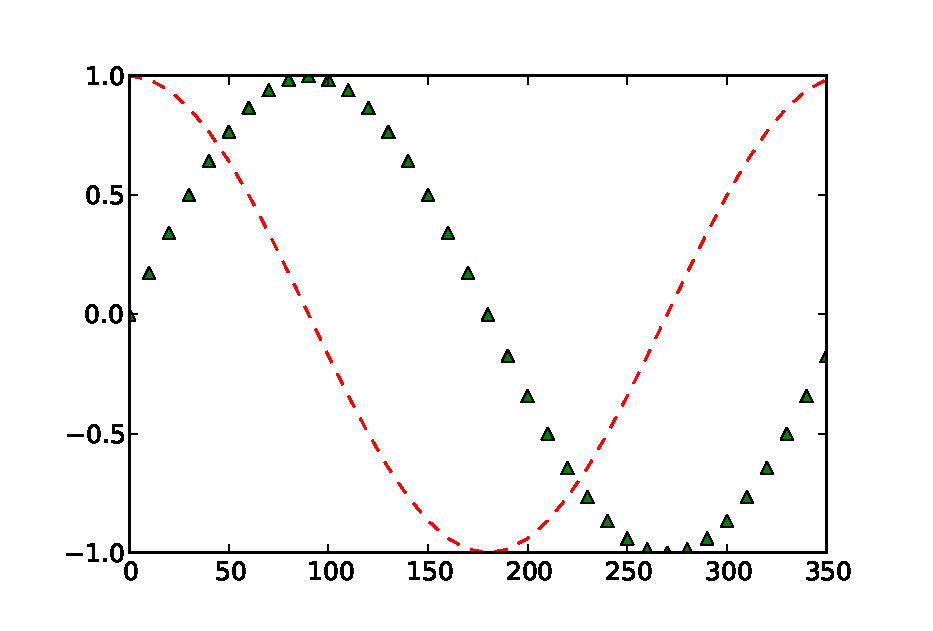
\includegraphics[width=5in]{figures/matplotlib2.eps}

\noindent   From the code, you can probably figure out that a line style of 'r--' is a red dashed line,  and 'g\verb|^|'  are green triangles.  
There are many other attributes that can be controlled: linewidth, dash style, etc. and I invite you to check out the {\color{blue}matplotlib} documentation.

\noindent By now, you should understand enough about classes, keyword argument passing and other pythonalia to be able to figure things out on your own.   But don't panic, I'm going to lead you through a few more examples, which I hope will speed you on your plotting way.  



\subsection{Multiple figures and more customization}
As already mentioned,  {\color{blue}pylab} has the concept of ``current figure'' which subsequent commands refer to.   In the preceding examples, we only had one figure, so we didn't have to name it, but for fancier figures with several plots, we 
can create  named figure objects by invoking a {\color{blue}figure} instance: 
 
 {\color{blue}\begin{verbatim}
fig = pylab.figure(num=1,figsize=(5,7)). 
\end{verbatim}}

\noindent  Notice the syntax whereby {\color{blue} figsize}  is a method with  width and height (in inches) specified by a tuple and {\color{blue}fignum}  is the figure number.    Notice that these are keyword arguments, and that there are many more:  consult the list of  **kwargs in the online documentation  located here:

 http://matplotlib.sourceforge.net/api/pyplot\_api.html\#matplotlib.pyplot.figure 

Once we have a figure instance (sometimes called a ``container''), we can do all kinds of things, including adding subplots.  To do this, we can use the syntax:

{\color{blue}\begin{verbatim}
 fig.add_subplot(211) 
 \end{verbatim}}
 \noindent Here the 
argument  211 means 2 rows, one column and this is the first plot.  To make plots side by side, you would use: {\color{blue} fig.add\_subplot(121) } for  1 row, two columns, etc.  

After each {\color{blue}add\_subplot} command, that subplot becomes the current figure for plotting on.
If you want more freedom, say, you want to make a subplot at an arbitrary place,  use the {\color{blue}add\_axes([left, bottom,width, height])} 0 method, e.g.,  {{\color{blue}add\_axes([0.1,0.1,0.7,0.3])}.  The values are 0-1 in relative figure coordinates. 

To illustrate these new concepts, consider the example code, {\color{blue}matplotlib3.py}:

{\singlespacing \color{blue} \begin{verbatim}
#!/usr/bin/env python
import matplotlib
matplotlib.use("TkAgg")
import pylab, numpy
def f(t):
    return numpy.exp(-t)*numpy.cos(2.*numpy.pi*t)
t1= numpy.arange(0.,5.,0.1)
t2= numpy.arange(0.,5.,0.02)
fig=pylab.figure(num=1,figsize=(7,5)) 
fig.add_subplot(211) 
pylab.plot(t1,f(t1),'bo')
pylab.plot(t1,f(t1),'k-') 
fig.add_subplot(212) 
pylab.plot(t2,numpy.cos(2*numpy.pi*t2),'r--')
pylab.xlabel('Time (ms)')
fig.add_axes([.6,.75,.25,.10])
pylab.plot([0,1],[0,1],'r-',[0,1],[1,0],'r-')
pylab.ylabel('Inset')
pylab.show()
\end{verbatim}}

\noindent which produces:

{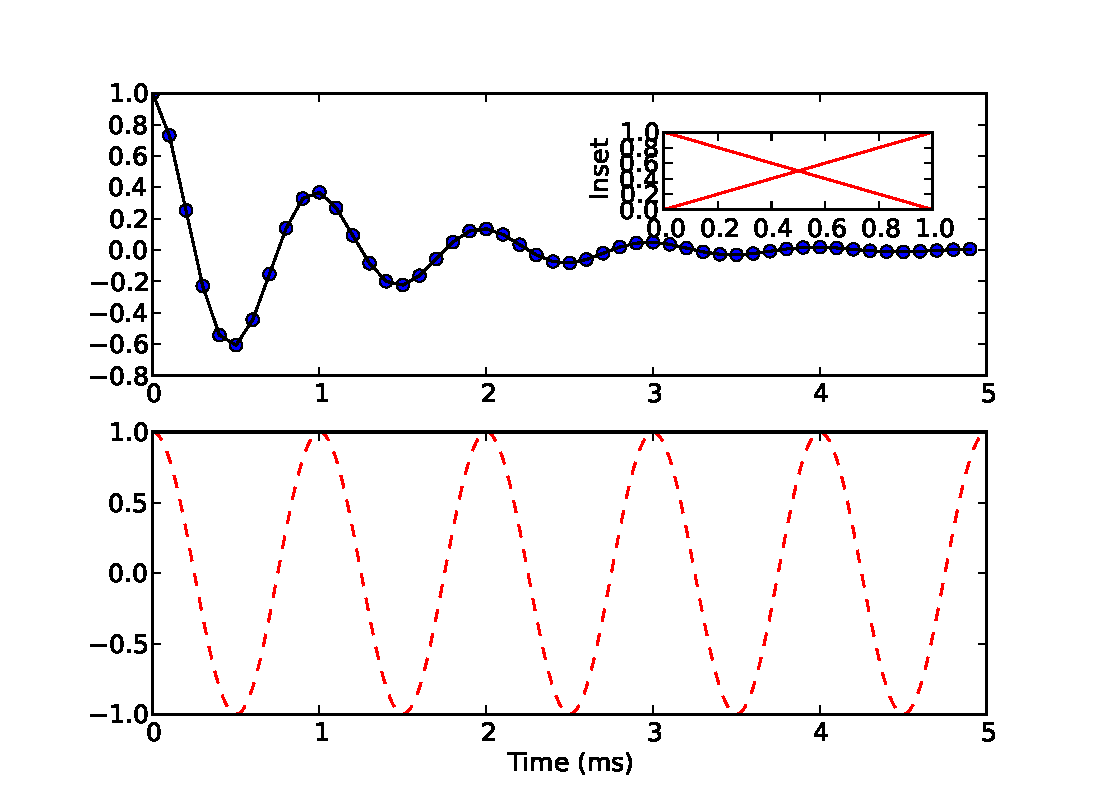
\includegraphics[width=5in]{figures/matplotlib3.eps}}

\noindent By now, you should be able to figure out what everything in that script does by yourself!  

\subsection{Adding text}

We already met {\color{blue}xlabel} and {{\color{blue}ylabel}.  But text can be added in a other ways, e.g., using the  title, text, legend and arrow methods.
Let's decorate one of our early examples to show how some of these things work:

{\singlespacing \color{blue} \begin{verbatim}
#!/usr/bin/env python
import matplotlib
matplotlib.use("TkAgg")
import pylab,numpy
x=numpy.arange(0,360,10)
r=x*numpy.pi/180.
c=numpy.cos(r)
s=numpy.sin(r)
s2=numpy.sin(r)**2
pylab.plot(x,c,'r--',x,s,'g^',x,s2,'k-')
pylab.title('Fun with trig')
pylab.text(250,-.5,'pithy note')
pylab.legend(['cos(x)',\
    'sin(x)',r'$\sin(x^2$)'],'lower left')
pylab.xlabel(r'$\theta')
pylab.annotate('triangles!',\
  xy=(175,0),xytext=(110,-.25),\
   arrowprops=dict(facecolor='black',\
   shrink=0.05))
pylab.show()
\end{verbatim}}

\noindent which produces this plot:

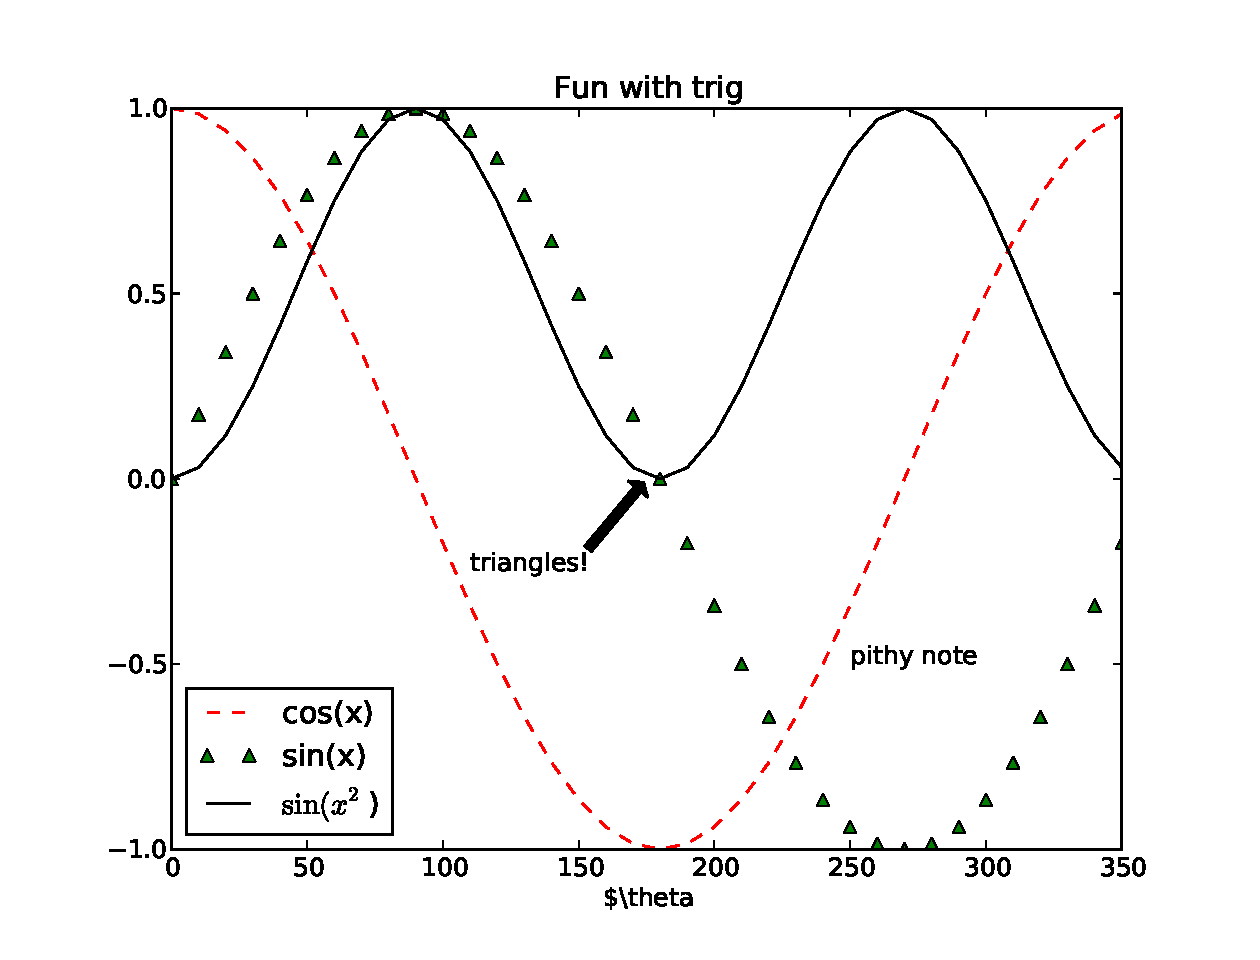
\includegraphics[width=4in]{figures/matplotlib4.eps}

The title appears at the top of the plot.  
    Text labels get places at the $x$ and $y$ coordinates on the plot and the legend will appear in the upper/lower right/left corner as specified in the string.  The {\color{blue}pylab.text(x,y,string, kwargs)} method also has optional key word arguments, specifying font, size, color and the like.     The legend 'labelist' is a list of labels for each plot element.  So, every line or point style that you want in your legend, append a label to the label list after the relevant plot command. Also note that the legend and xlabel methods use  a special format for strings ({\color{blue}r'LateX String')} which allows embedded LaTeX equation syntax  to make scientific equations look right - so now you have to learn LaTeX!.   Finally, the arrow gets drawn with the {\color{blue}annotate} method, which has a lot of other attributes as well.
Check the {\color{blue}matplotlib} documentation for details.  
    




There are lots of graphing styles possible with {\color{blue}matplotlib}, e.g., histograms, pie charts, contour plots, whisker plots, etc.  I'm just going to show you a few examples.  The best thing to do is to look through the online documentation for a plot that looks like what you need, then modify it.  This is ALWAYS a good approach - start with something that works and fiddle with it until it suits your own particular needs.  



\noindent
{\singlespacing \color{red}ASSIGNMENT P6

The file SPECMAP.dat has $\delta^{18}O$ data versus age (in ka). For those of you who don't know, this is  classic  record of Imbrie et al., 1984 variations in oxygen isotopic ratio of seawater controlled by changes in global ice volume which in turn was forced by the Earth's orbit.    Write a Python program that :
\begin{itemize}
\item  reads in the data and 
\item makes a simple X,Y plot with symbols connected by lines
\item  put Age on the X axis and  $\delta^{18}O$ on the Y.  -the LaTeX code for $\delta^{18}O$ is:
\begin{verbatim}
$\delta^{18}O$ 
\end{verbatim}
\item  send the script to me at ltauxe@ucsd.edu 
\end{itemize}
}





\subsection{Histograms}

%%\vskip -.3in
I downloaded a week's worth of earthquake location, magnitude etc. from the website: 

http://earthquake.usgs.gov/earthquakes/catalogs/index.php

\noindent by clicking on the ``XML merged catalog, past 7 days''  link.  

\noindent This a compressed (gnu zip)  XML file. After unzipping it (by clicking on it), the file (called {\color{blue}merged\_catalog.xml} looked something like this:

{\singlespacing \begin{verbatim}
<?xml version="1.0" encoding="UTF-8"?>
<merge>
    <event id="71672091" network-code="NC"
        time-stamp="2011/11/03_23:03:32 " version="2">
        <param name="year" value="2011"/>
        <param name="month" value="10"/>
        <param name="day" value="28"/>
        <param name="hour" value="21"/>
        <param name="minute" value="21"/>
        <param name="second" value="52.7"/>
        <param name="latitude" value="38.8147"/>
        <param name="longitude" value="-122.7862"/>
        <param name="depth" value="1.7"/>
        <param name="magnitude" value="0.2"/>
        <param name="num-phases" value="8"/>
        <param name="dist-first-station" value="0.0"/>
        <param name="rms-error" value="0.00"/>
        <param name="hor-error" value="0.8"/>
        <param name="ver-error" value="0.6"/>
        <param name="azimuthal-gap" value="42"/>
        <param name="magnitude-type" value="D"/>
        <param name="magnitude-type-ext" value="Mcd = coda duration magnitude"/>
        <param name="num-stations-mag" value="3"/>
        <param name="stand-mag-error" value="0.1"/>
        <param name="location-method" value="h"/>
        <param name="location-method-ext" value="Hypoinverse (Confirmed by human review)"/>
    </event>
    <event id="71672096" network-code="NC"
        time-stamp="2011/10/28_21:30:19 " version="0">
        <param name="year" value="2011"/>
        <param name="month" value="10"/>
etc.
\end{verbatim}}


Reading in all the data, I can plot them various ways.  In this example, I plot a histogram of the magnitudes:

{\singlespacing \color{blue} \begin{verbatim}
#!/usr/bin/env python
import matplotlib
matplotlib.use("TkAgg")
import pylab
def readEQs(infile):
    input=open(infile,'rU').readlines()
    EQs=[] # list to put EQ dictionaries in
    linenum=0
    while linenum <len(input):
        if 'event id' in input[linenum]: # new event
            EQ={} # define a dictionary
            linenum+=2 # increment past time-stamp
            while 'param' in input[linenum]:
                record=input[linenum].split('=')
                datakey=record[1].split()[0].strip('"')
                EQ[datakey]=record[2].strip('\n').strip('/>').strip('"')
                linenum+=1 # keep going until </event>
            if '</event>' in input[linenum]: # done with event
                EQs.append(EQ)
        linenum+=1 # look for next event id
    return EQs
EQs=readEQs('merged_catalog.xml')
Magnitudes=[] # set up container
for eq in EQs: # step through earthquake dictionaries
    Magnitudes.append(float(eq['magnitude'])) # collect magnitudes
pylab.hist(Magnitudes,bins=50,normed=True) # plot 'em
pylab.xlabel('Richter Magnitude')
pylab.ylabel('Frequency')
pylab.show()  
\end{verbatim}}

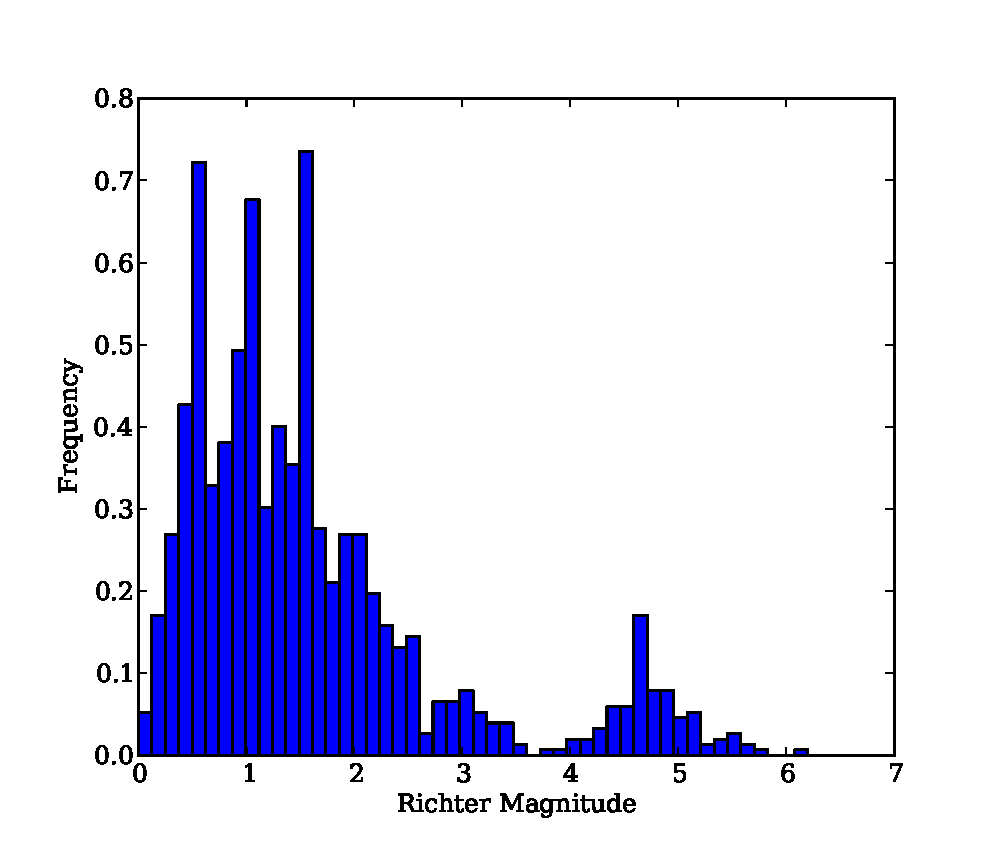
\includegraphics[width=4in]{figures/matplotlib5.eps}

\noindent
In the example, please notice the clever way in which we parse the XML code.  First, we look for the new event marker, then split the record on its '='.  This gives a element list with what we need.  The second element contains the key and the third element the value.  To get the key name, we split on the space which puts the key name (which puts the key name enclosed in quotes in the first element of a list, which we select and strip off the quotes.  This we use as the key in the dictionary, EQ.  To get the value, we use the third element in the 'record' list (record[2]), strip off the end of line character and the quotes.  We pair the value with the key in the EQ dictionary and continue, incrementing linenum until we have all the keys picked off and hit the '$<$even$t>$' line.  When we are done with a dictionary, we append it to a list of all the dictionaries, increment linenum and press on.  We keep going until we have read all the data.  

After we have parsed the data file into a list of dictionaries, we make a list for the thing we one to plot (Magnitudes), hunt through the list, picking out the magnitude data and after turning it into a float, append it to the list.  We plot the histogram using the {\color{blue}pylab.hist} method.  We can label the plot as per usual and display it with {\color{blue}show()}.     The dictionaries get appended to a list.  This way, any particular key could easily get fished out later for plotting.  In this case, we just put the float of the 'Magnitude' column into the list Magnitudes.  These get plotted in the histogram.  
\subsection{Pie Charts}

I mostly think pie charts are silly, but some people love them.  So if you want to see  data as a pie chart, say the fraction of earthquakes in each magnitude bin from the last example, we can modify the script thusly:


{\singlespacing \color{blue} \begin{verbatim}
#!/usr/bin/env python
import matplotlib
matplotlib.use("TkAgg")
import pylab
from readEQs import *
EQs=readEQs('merged_catalog.xml')
Fracs,Labels=[],[]
bin0=0
for m in range(1,8):  # assume no magnitudes bigger than 8 last week!
    num=0 # initialize count
    for eq in EQs:
        eqm=float(eq['magnitude'])
        if eqm<m and eqm>bin0:num+=1 # count all magnitudes in this bin
    Fracs.append(float(num))
    Labels.append(str(bin0)+'-'+str(m))
    bin0=m # increment to next bin
pylab.pie(Fracs, labels=Labels) 
pylab.axis('equal') # make the pie round!
pylab.title('Silly Pie Chart')
pylab.show()  
\end{verbatim}}
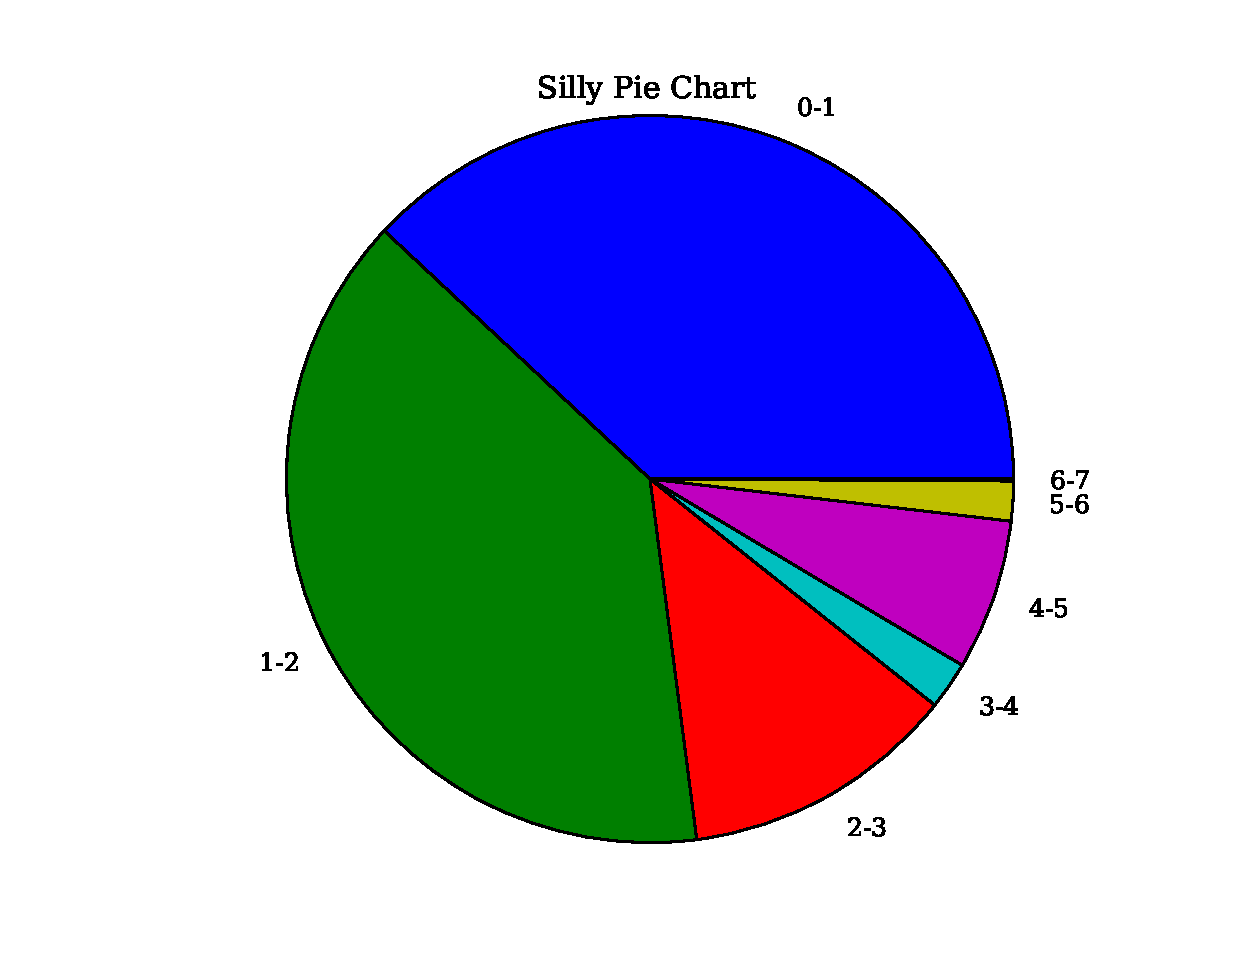
\includegraphics[width=4in]{figures/matplotlib6.eps}}

\noindent Notice how the function {\color{blue}readEQs} from the histogram example has been put into a module by itself and then called within this program.  



\subsection{Basemap}

Most of your maps can be made  with GMT, but python can make maps too.   Once you know Python, it can be much easier to use GMT because the same principles apply and all of the power of {\color{blue}matplotlib} is available for enhancing your plots.  We generate maps with a special ``toolkit'' of {\color{blue}matplotlib}  called {\color{blue}Basemap}.     


Here is a simple example, using our earthquake data from the histogram example to make a mollweide projection with the earthquake locations as red dots.


{\singlespacing \color{blue} \begin{verbatim}
#!/usr/bin/env python
import matplotlib
matplotlib.use("TkAgg")
import pylab,numpy
from readEQs import *
from mpl_toolkits.basemap import Basemap
EQs=readEQs('merged_catalog.xml') # read in data (see histogram example)
Lats,Lons=[],[] # set up lists for location data
for eq in EQs: # step through the list of earthquakes
    Lats.append(float(eq['latitude'])) # collect the latitudes (as floats)
    Lons.append(float(eq['longitude']))
map=Basemap(projection='moll',lon_0=0,resolution='c') # create a map instance
map.drawcoastlines()
map.drawmapboundary()
map.drawmeridians(numpy.arange(0,360,30)) # draws longitudes from list
map.drawparallels(numpy.arange(-60,90,30)) # draws latitudes from list
X,Y=map(Lons,Lats) # calculates the projection of the X,Y
pylab.plot(X,Y,'ro') # uses pylab's plot to plot these arrays
pylab.savefig(map.eps) # save the figure in EPS format
\end{verbatim}}

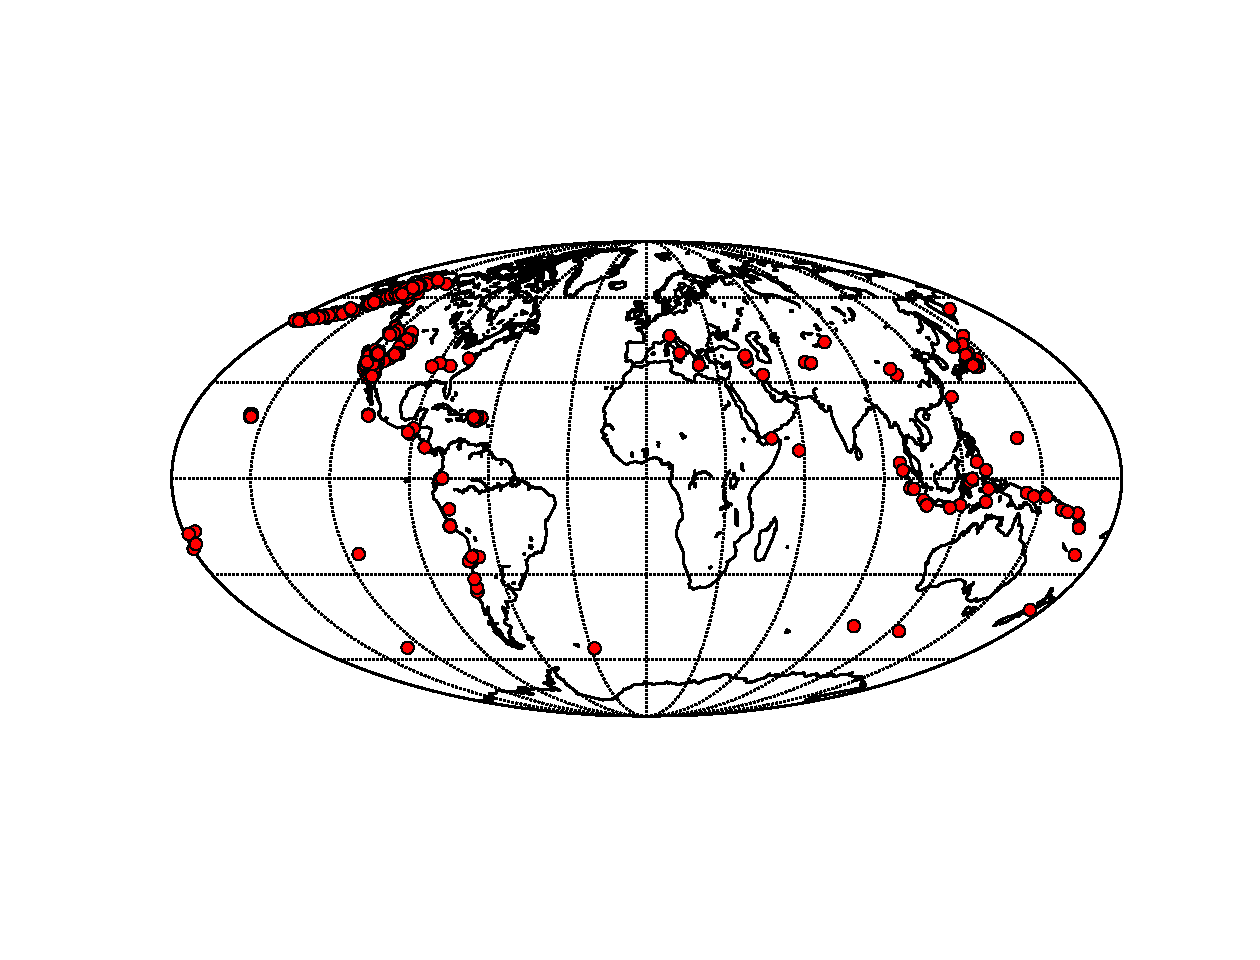
\includegraphics[width=4in]{figures/matplotlib7.eps}

\noindent
In this example, the list of earthquake dictionaries, {\color{blue}EQs} is read in with the same file reading function from the histogram example.   Then we fish out the latitude and longitudes from each earthquake dictionary ({\color{blue}eq}) and append the floating point equivalent (remember they are strings in the dictionary!) into the relevant lists (Lats, Lons).  

The basic concept of Basemap is that you create a map class instance with a call to {\color{blue}Basemap}.  The attributes of you map (e.g., resolution, projection, central longitudes, map boundaries, map center, etc.), i.e., all the things you set with switches in {\color{blue}pscoast} are set with keyword arguments in the call to Basemap.  The details of these key word arguments depend on the projection you choose.  

After you create the map instance (called {\color{blue}map}) in the above example, you can modify attributes in using methods available to this particular subclass.  To draw the coastlines, use the method {\color{blue}drawcoastlines()}.  To draw the lines of longitude we use the method {\color{blue}drawmeridians()} with the an array (or list) containing the longitudes you want to plot. In this case we generated the array with {\color{blue}numpy.arange}, but we could have used {\color{blue}range(0,360,30)} or any arbitrary integer or floating point list.  
Drawing the lines of latitude works the same way (with the {\color{blue}drawparallels()} method).

Now we want to plot a bunch of points on the map.  By sending in the longitudes and latitudes of the earthquake locations as arguments to the map class, the class chews on them and spits out $x$,$y$ values based on the projection we specified when creating the map instance with Basemap.  Now we can plot the returned {\color{blue}X, Y} lists using the `regular' {\color{blue}pylab} plotting functions.  We can go on and decorate the map with anything available in {\color{blue}pylab}.  
The advantage of using {\color{blue}Basemap} over, say, GMT is you can build on your knowledge of {\color{blue}matplotlib}, instead of struggling with two completely different and incompatible plotting packages.  

For more examples, check the documentation available here: 

http://matplotlib.github.com/basemap/users/examples.html



{\color{red}

\noindent ASSIGNMENT P7

Redo your GMT1 assignment using the {\color{blue}Basemap} toolkit!.  Add a point labelled ``Now I'm here!'' and the location of SIO.
}


\subsection{Contour plots}

Of the many plotting methods available in {\color{blue}matplotlib}, one of the more useful for Earth Scientists is the contour plot.  Here is a example of the gravity anomaly created by a buried sphere:


{\singlespacing \color{blue}\begin{verbatim}
#!/usr/bin/env python
import numpy
import matplotlib
matplotlib.use("TkAgg")
import pylab
G=6.67e-11 # grav constant in Nm^2/kg^2 (SI)
R=2. # radius in meters
z=3. # depth of burial
drho=500 # density contrast in kg/m^3
x=numpy.arange(-2.*z,2.*z,0.1)
y=numpy.arange(-2.*z,2.*z,0.1)
X,Y=pylab.meshgrid(x,y)
h=numpy.sqrt(X**2+Y**2) 
g=(G*4.*numpy.pi*R**3.*drho)/(3.*(h**2+z**2))
pylab.imshow(g,interpolation='bilinear',cmap=pylab.cm.Spectral)
pylab.colorbar()
pylab.axis('equal')
pylab.show()
\end{verbatim}}


{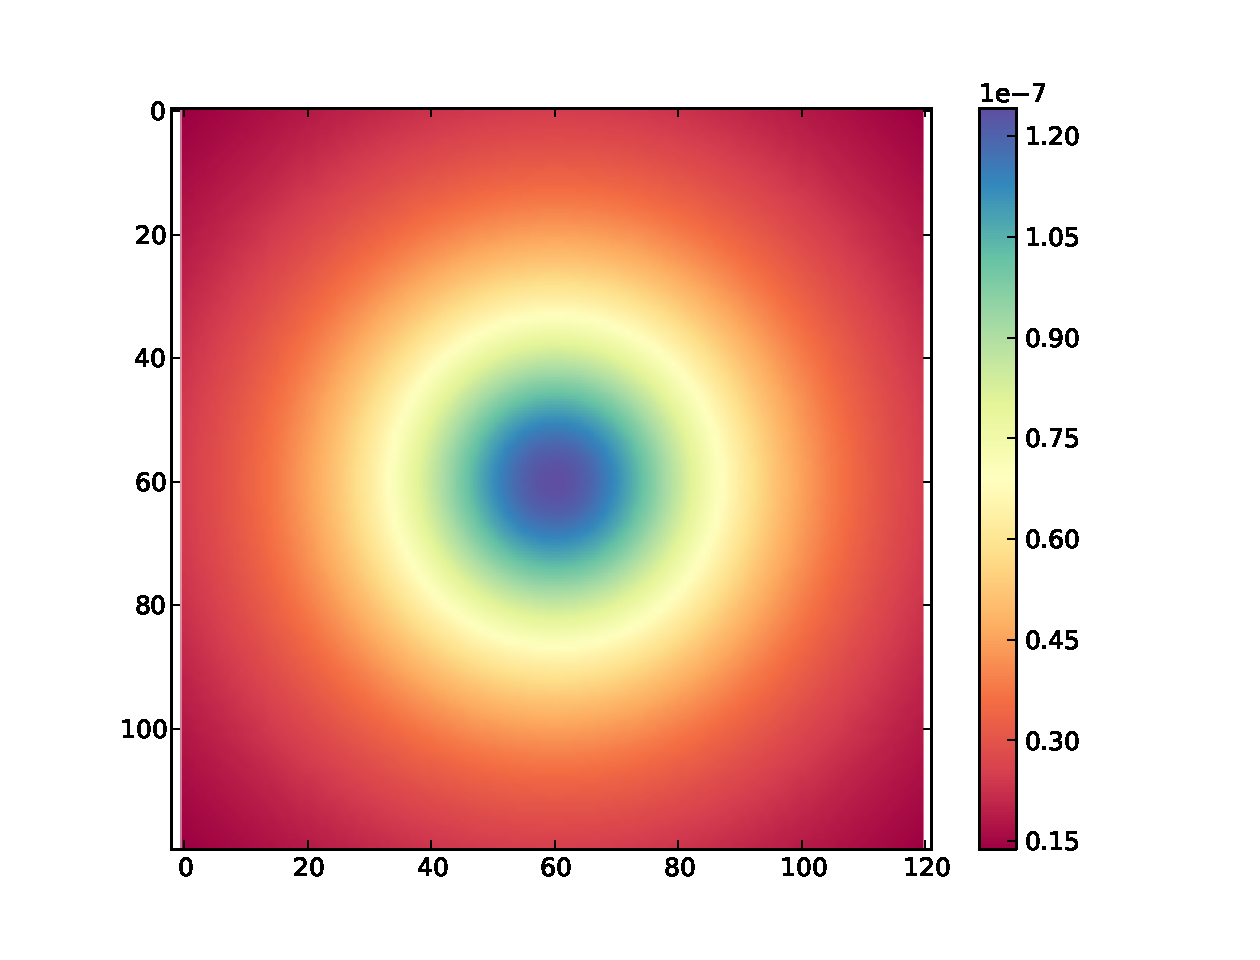
\includegraphics[width=4in]{figures/matplotlib8.eps}}

The first new function for us in the above example is {\color{blue}meshgrid}.  This makes 2D arrays {\color{blue}X} and {\color{blue}Y}  for a 3D mesh/surface plots.    These have the dimensions of $x$ by $y$.  Each row of {\color{blue}X} is the same as $x$ and there is a row for every element in $y$. Similarly, each column in  \color{blue}Y} is a copy of $y$ and there is a column for every element in $x$.  

The line {\color{blue}h=numpy.sqrt(X**2+Y**2)} calculates the horizontal distance $h$ from the origin for every point on the  {\color{blue}X,Y} grid.   Then we calculate the gravity anomaly $g$ for a spherical mass with radius ($R$) at depth of $z$ with the command:

 {\color{blue}\begin{verbatim}
 g=(G*4.*numpy.pi*R**3.*drho)/(3.*(h**2+z**2))
 \end{verbatim}}
 
\noindent You can find the formula for this in any geophysics text book.  Anyway, now we have $g$ which if you print it out, looks like this:

{\singlespacing \color{blue}\begin{verbatim}
[[  1.37971509e-08   1.40028722e-08   1.42112058e-08 ...,   1.44221090e-08
    1.42112058e-08   1.40028722e-08]
 [  1.40028722e-08   1.42148210e-08   1.44295575e-08 ...,   1.46470410e-08
    1.44295575e-08   1.42148210e-08]
 [  1.42112058e-08   1.44295575e-08   1.46508813e-08 ...,   1.48751394e-08
    1.46508813e-08   1.44295575e-08]
 ..., 
 [  1.44221090e-08   1.46470410e-08   1.48751394e-08 ...,   1.51063696e-08
    1.48751394e-08   1.46470410e-08]
 [  1.42112058e-08   1.44295575e-08   1.46508813e-08 ...,   1.48751394e-08
    1.46508813e-08   1.44295575e-08]
 [  1.40028722e-08   1.42148210e-08   1.44295575e-08 ...,   1.46470410e-08
    1.44295575e-08   1.42148210e-08]]
\end{verbatim}}

\noindent
It is a 2D array in which every element is the value of $g$ at that grid point.  There are a bunch of ways to visualize this, but here we plot it as a contour plot.  To do this we interpolate between all the grid points and choose a color map translating the value of $g$ into a color from blue to orange.  When choosing color maps, be aware that a lot of people are red-green color blind and appreciate some other color contrast, like the  blue-orange one chosen here.






\section{Deeper into NumPy and Scipy}

Now we have some plotting skills under our belt, we can take advantage of the computational tools available in {\color{blue}NumPy} and another scientific package called {\color{blue}Scipy}.  
We have already met these: cos(), sin(), pi(), arctan2(), arange(), among others.  
 Now meet {\color{blue}polyfit(x,y,order)}, and {\color{blue}polyval(coeffs,x)}. The former fits an n-order polynomial to input data and returns a list of the coefficients and the latter evaluates the value at x using coefficients returned from polyfit.  
 
To find a best fit line ($y=mx+b$ where $m$ is the slope and $b$ is the intercept) we can  use {\color{blue}polyfit()} by setting  for {\color{blue}order} to one.  Order is two for  a quadratic polynomial, ($y=ax^2+bx+c$) and three for cubic  ($y=ax^3+bx^2+cx+d$).  See how these work in the following example: 


{\singlespacing \color{blue} \begin{verbatim}
#!/usr/bin/env python
import matplotlib
matplotlib.use("TkAgg")
import numpy,pylab
from numpy import random
x,y=[1.,2.,3.,4.],[1.,1.8,3.4,4.2] # defines two lists
X=numpy.arange(x[0],x[-1]+.5,.1)
pylab.plot(x,y,'ro')
coeffs=numpy.polyfit(x,y,1)
Y=numpy.polyval(coeffs,X)
pylab.plot(X,Y,'r-')
y2=[3.42, 11.24, 19.86, 34.87]
pylab.plot(x,y2,'bs')
coeffs2=numpy.polyfit(x,y2,2)
Y2=numpy.polyval(coeffs2,X)
pylab.plot(X,Y2,'b-')
pylab.show()
\end{verbatim}}

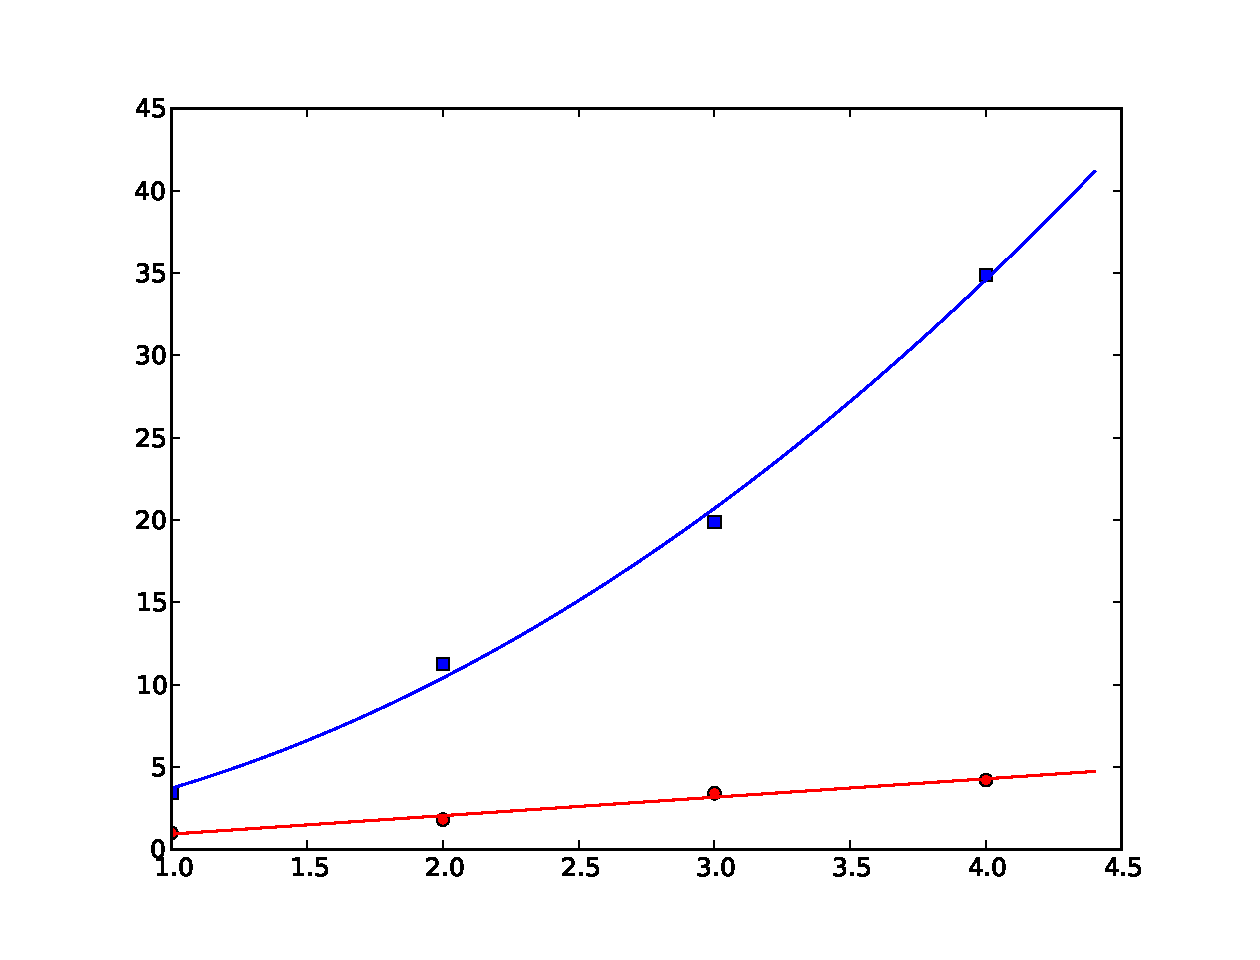
\includegraphics[width=5in]{figures/numpy1.eps}

\noindent
In the first call to the  function {\color{blue}polyfit()}, it returns a list {\color{blue}coeffs=[ 1.12 -0.2 ]}, with the coefficients $m$ and $b$;  strangely  it has no commas, so be careful.  This list can be passed directly into  {\color{blue}polyval()}, which returns the $y$ values evaluated at the positions in the $X$ list (or array) that is passed in.  We plot these values as the red line, compared to the original data points ($x,y$) which are red dots.   

In the second call to the function {\color{blue}polyfit()}, we sent it new values for $y$ ($y2$) and asked for a second order polynomial fit.  {\color{blue}coeffs2} is   [ 1.7975  1.3095  0.5925] which are $a,b, c$  respectively.   This in turn gets churned through {\color{blue}polyval()} and plotted as the blue curve (as compared to $y2$ which are the blue dots).  


\subsection {More on slicing with arrays}

 We zoomed by the finer points of list and array indexing earlier in the chapter, eager to get to plotting.  Now we delve deeper.

First a review of lists.   You will recall that in  python, indexing starts with 0, so for the list {\color{blue} L=[0,2,4,6,8], L[1]} is 2. The index of the last item is -1, so  {\color{blue}L[-1]}=8.  To find out what the index for the number 4 is, for example, we have the {\color{blue}index()} method:  {\color{blue}L.index(4}), which will return the number 2. We actually already used this method when we implemented command line arguments, but it wasn't really explained.   We know that to reassign a given index a new value we use the syntax {\color{blue}L[1]=2.5}.  
And to use a part of a list (a slice) we use, e.g.,    {\color{blue}B=L[2:4]}, which  defines  {\color{blue}B} as a list with  {\color{blue}L}'s elements 2 and 3 (4 and 6).  And you also know that  {\color{blue}B=L[2:]} takes all the elements from 2 to the end.  
From these examples, you can infer that the basic syntax for slicing is  {\color{blue}[start:stop:step]}; if the step is omitted it is assumed to be 1.  

Arrays (and matrices) work in a similar fashion to lists, but these are multidimensional objects, so things get hairy fast.
The basic syntax is the same:  {\color{blue}[start:stop:step]},  or  {\color{blue}i:j:k}.   but with Python arrays, we step through all the  {\color{blue}j}'s for each  {\color{blue}i}  at step  {\color{blue}k}.  This is best shown with examples:


{\singlespacing \color{blue} \begin{verbatim}
>>> import numpy
>>> A=numpy.linspace(0,29,30)
>>> B=A.reshape(5,6)
array([[  0.,   1.,   2.,   3.,   4.,   5.],
       [  6.,   7.,   8.,   9.,  10.,  11.],
       [ 12.,  13.,  14.,  15.,  16.,  17.],
       [ 18.,  19.,  20.,  21.,  22.,  23.],
       [ 24.,  25.,  26.,  27.,  28.,  29.]])
>>> B[1:3,:-1:2] 
array([[  6.,   8.,  10.],
       [ 12.,  14.,  16.]])
\end{verbatim}}

Let's pick about the statement {\color{blue}B[1:3,:-1:2]} to see if we can understand what it does.  The first part alone returns lines 2 and 3:
{\singlespacing \color{blue} \begin{verbatim}
>>> B[1:3]
array([[  6.,   7.,   8.,   9.,  10.,  11.],
       [ 12.,  13.,  14.,  15.,  16.,  17.]])
\end{verbatim}}

Here  {\color{blue}j} goes from [:-1], in other words, we all but the last element:

{\singlespacing \color{blue} \begin{verbatim}
>>> B[1:3,:-1]
array([[  6.,   7.,   8.,   9.,  10.],
       [ 12.,  13.,  14.,  15.,  16.]])
\end{verbatim}}

\noindent And finally, we have the step of 2, which takes every other element:

{\singlespacing \color{blue} \begin{verbatim}
>>> B[1:3,:-1:2] 
array([[  6.,   8.,  10.],
       [ 12.,  14.,  16.]])
\end{verbatim}}

\noindent For more on array slicing (indexing), see:

http://docs.scipy.org/doc/numpy/reference/arrays.indexing.html




\subsection{Looping through arrays}

 Earlier in the course, we learned that  {\color{blue} for} loops with lists  just step through item by item.  In n-dimensional arrays, they steps through row by row (like in slicing).  For example, 
 

{\singlespacing \color{blue} \begin{verbatim}
>>> for r in B:
...    print r
... 
[ 0.  1.  2.  3.  4.  5.]
[  6.   7.   8.   9.  10.  11.]
[ 12.  13.  14.  15.  16.  17.]
[ 18.  19.  20.  21.  22.  23.]
[ 24.  25.  26.  27.  28.  29.]
\end{verbatim}}

If you really want to step through element by element, you can use the {\color{blue}ravel()} method which flattens an N-dimensional array to a single dimension:

{\singlespacing \color{blue} \begin{verbatim}
>>> for e in B.ravel():
...    print  e
... 
0.0
1.0
2.0
3.0
etc.
\end{verbatim}}

For more on looping (or iterating), see:

http://docs.scipy.org/doc/numpy/reference/arrays.nditer.html

\subsection{Random Numbers}

Many scientific investigations use techniques such as Monte Carlo simulations, or bootstrap statistics, which you (hopefully) will learn about in future classes.  These applications require that you be able to generate random numbers from a variety of distributions.  Python does this with the {\color{blue}numpy.random} module.  To learn more, read the documentation at:

http://docs.scipy.org/doc/numpy/reference/routines.random.html

Let's look at a few of these: 


{\singlespacing \color{blue} \begin{verbatim}
#!/usr/bin/env python
import matplotlib
matplotlib.use("TkAgg")
import pylab
from numpy import random
N,min,max=500,10,20
bins=(max-min)*2
Nums=[]
for n in range(N):
    Nums.append(random.uniform(min,max))
pylab.hist(Nums,bins=bins,facecolor='orange')
pylab.title('Uniform distribution')
pylab.show()
\end{verbatim}}

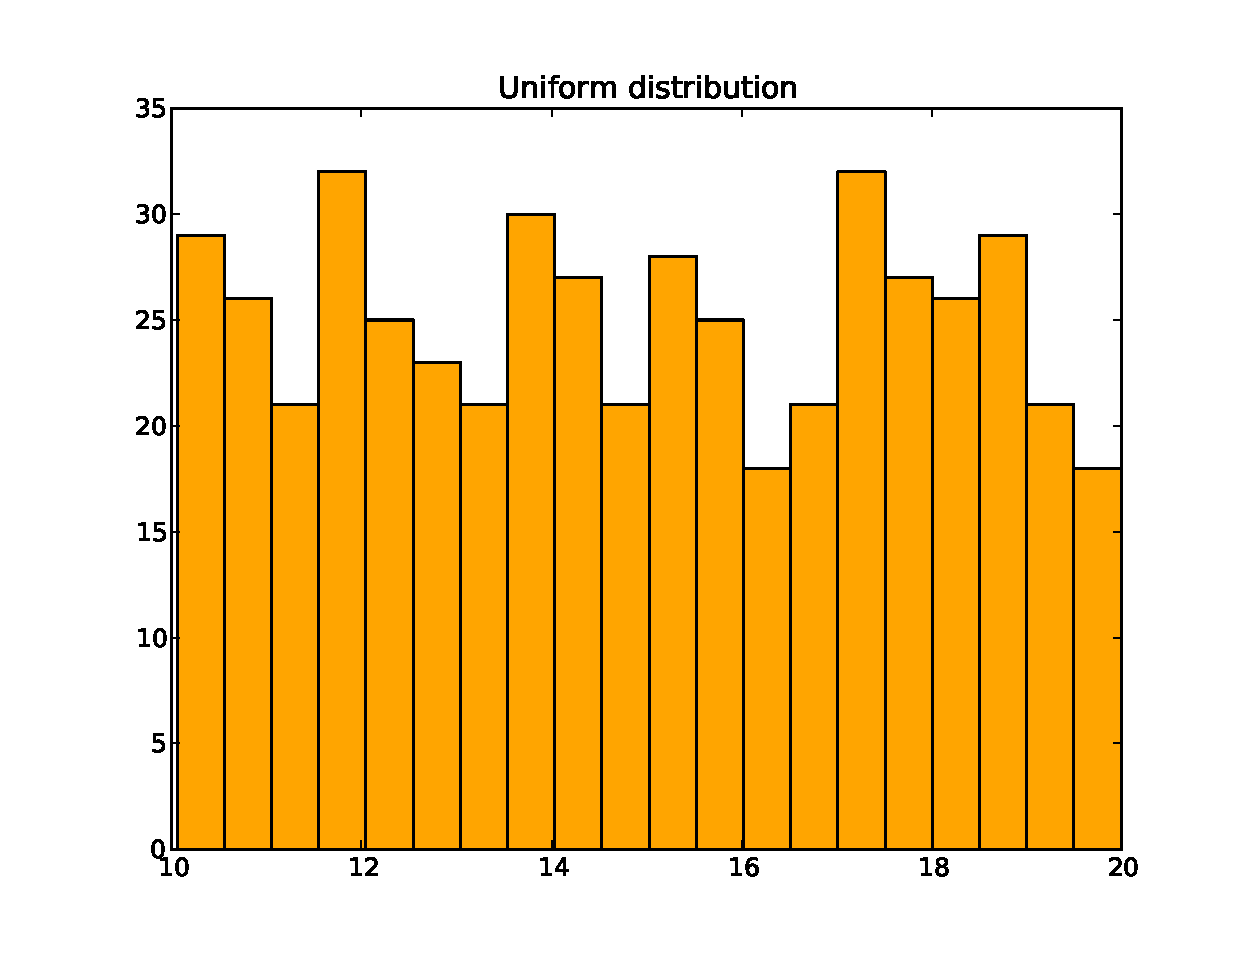
\includegraphics[width=5in]{figures/numpy2.eps}

\noindent The new twist here is the call to the {\color{blue}uniform()} method of the {\color{blue}random()} module of {\color{blue}NumPy}.  This returns uniformly distributed numbers between the min and max values specified.  The other embellishments were to the {\color{blue}hist()} module in {\color{blue}matplotlib} by increasing the number of bins (the default is too few in my opinion) and to change the color of the columns to a pretty shade of orange.  


\subsection{Normal Distribution}

There are dozens of other distributions available in the {\color{blue}random} module, but the all time favorite is the normal, or Gaussian distribution.  Here we have an example of how to use it to retrieve numbers from a normal distribution  with a mean of 10 and a standard deviation of 2:


{\singlespacing \color{blue} \begin{verbatim}
#!/usr/bin/env python
import matplotlib
matplotlib.use("TkAgg")
import pylab
from numpy import random
N,mu,sigma=500,10,2
Nums=[]
for i in range(N):
    Nums.append(random.normal(mu,sigma))
pylab.hist(Nums,bins=20,facecolor='orange')
pylab.title('Normal distribution')
pylab.show()
\end{verbatim}}

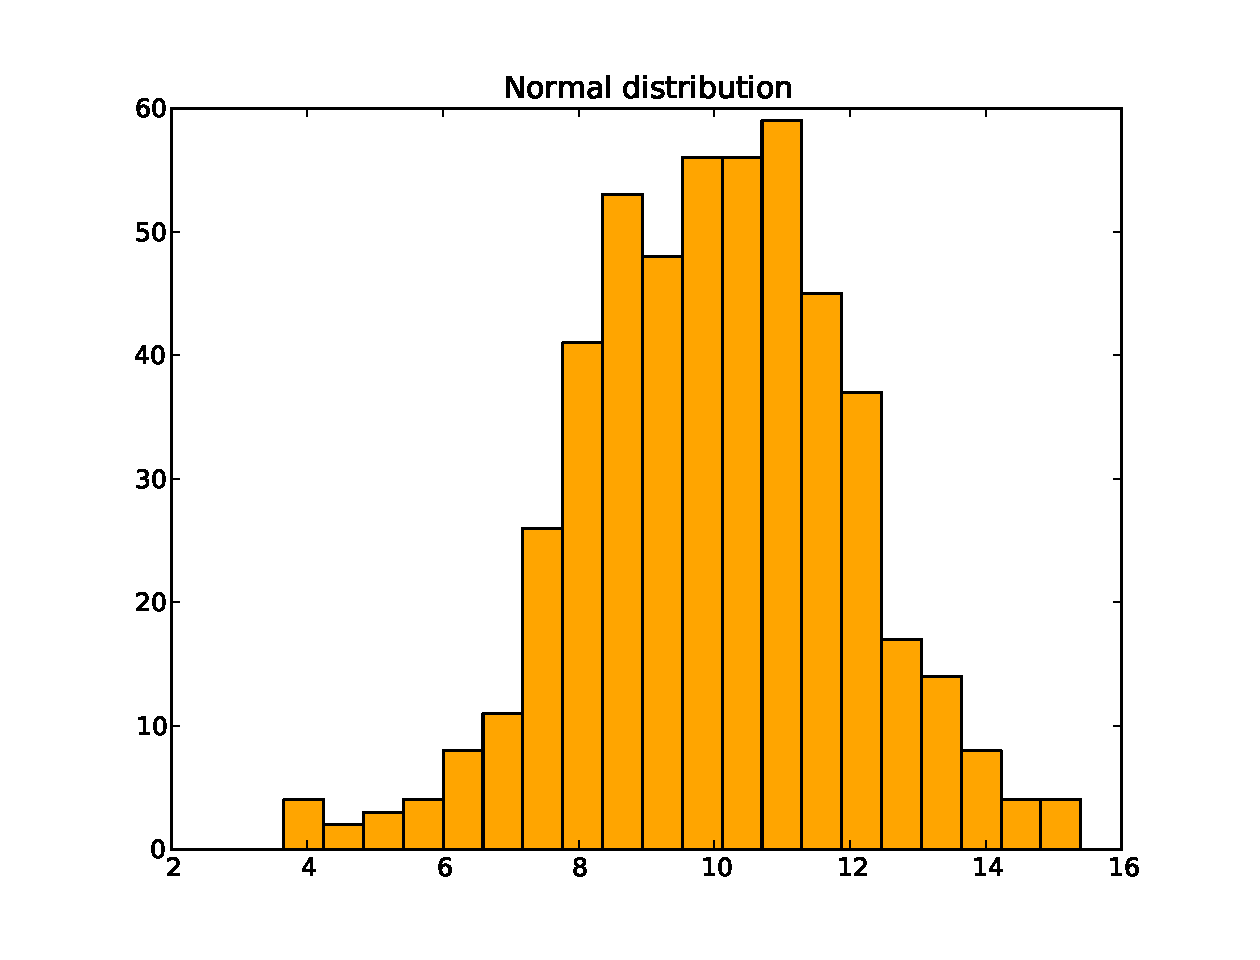
\includegraphics[width=4.5in]{figures/numpy3.eps}

\subsection{Statistics in Python}

All this talk about normal distributions makes me hungry for some statistical analysis.  
There are a large number of statistical packages available in the Enthought Python Distribution we are using for this class.  Numpy has a number of useful functions and there are many more hidden in the  {\color{blue}stats} module of the Scipy package.  For a summary of available functions, see:  
The documentation is still a bit thin, but to get you started, see:

http://docs.scipy.org/doc/numpy/reference/routines.statistics.html

and

http://docs.scipy.org/doc/scipy/reference/stats.html

Here we will consider a few  useful functions to give you a feel for how they work.  Let's start with 1D arrays and find the mean, standard deviation and sum.  For fun, we can use some of the fake data generated by the random.normal() function and see how the  actual means and standard deviations of a data set drawn from a normal distribution compare with the  true mean of $\mu$ and standard deviation $\sigma$.  

From the normal distribution example, we generated a list of numbers drawn from a distribution with $\mu=10$ and $sigma=2$:

{\color{blue}\begin{verbatim}
#!/usr/bin/env python
import numpy
from numpy import random
N,mu,sigma=500,10,2
Nums=[]
for i in range(N):
    Nums.append(random.normal(mu,sigma))
ANums=numpy.array(Nums)
print numpy.mean(ANums), numpy.std(ANums),numpy.sum(ANums)
\end{verbatim}}

\noindent
We wanted to calculate the mean, standard deviation and sum of our sample ({\color{blue}Nums} using the functions {\color{blue}numpy.mean(), numpy.std(), numpy.sum()}.  These work on arrays, not lists, so we first convert to an array:  {\color{blue}ANums=numpy.array(Nums)}.   When we run this code, we get:

{\color{blue}\begin{verbatim}
10.0428129458 2.0027306608 5021.40647292
\end{verbatim}}

\noindent Note that you will get a different answer every time you run this because the random sample really is pretty random.  The mean and standard deviation here are 10.042....  and 2.0027, which are close to the true values of 10 and 2 respectively.  

{\color{red} \singlespacing

ASSIGNMENT P8:

Modify the statistics example above to calculate 1000 versions of Nums, with an $N$ of 10.  Calculate the mean and standard error (standard deviation/ $\sqrt N$) values for each sample.  Plot a histogram of the means.   
The  standard error times 1.96 is the 95\% confidence bound for the mean, i.e., the mean $\pm$ these bounds should contain the true mean (10) 95\% of the time.  For what  fraction of the 1000 samples is this true? 
}

We can also use the statistics methods on n-dimensional arrays.  Here, the argument can specify the axis along which we want to do the calculation.   Recalling the arrays from before, we can illustrate the use of the {\color{blue}numpy.sum()} function as follows:

{\color{blue}\begin{verbatim}
>>> A= numpy.array([[1,2,3],[4,2,0],[1,1,2]])
>>> A.sum(axis=0)
array([6, 5, 5])
>>> A.sum(axis=1)
array([6, 6, 4])
\end{verbatim}}



%We already saw how to generate fake data sets by drawing samples from specified distributions, and some simple statistical calculations.   With the {\color{blue}scipy.stats} module we also calculate the mean, standard deviation, skewness, kurtosis, probability density functions and cumulative distribution functions.   Let's try some of these for fun.

%


%\subsection{Two normal distributions and a probability density function}

%
%In the following example, we draw 500 samples each from normal distributions with two different means and standard deviations.  These two get stored in the list {\color{blue}fakedata}.  The function  {\color{blue}gaussian_kde} returns a probability density function for the data, 

%{\singlespacing \color{blue} \begin{verbatim}
%#!/usr/bin/env python
%import matplotlib
%matplotlib.use("TkAgg")
%import pylab
%from numpy import linspace, min, max, random
%from scipy.stats import gaussian_kde
%fakedata=[]
%N=500
%for i in range(N): fakedata.append(random.normal(0.,1.))
%for i in range(N): fakedata.append(random.normal(4.,0.8))
%pdf=gaussian_kde(fakedata) # gaussian kernal density estimate
%x=linspace(min(fakedata),max(fakedata),len(fakedata))
%pylab.hist(fakedata,bins=N/5,normed=Truje)
%pylab.plot(x,pdf(x),'r') # probability density function
%pylab.show()
%\end{verbatim}}

%

%

%\subsection{The plot}
%And if you guessed this, you get 2 points:

%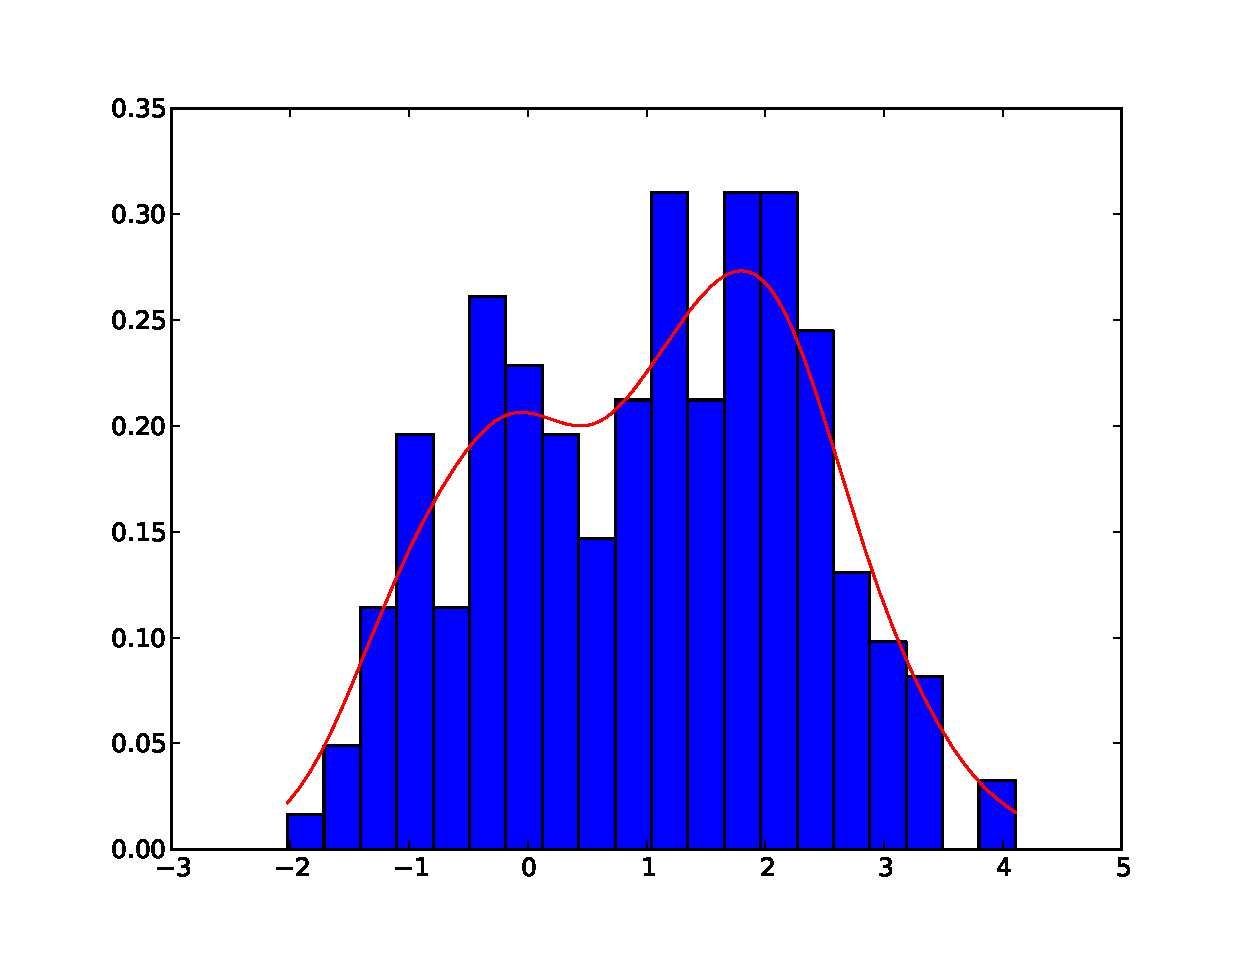
\includegraphics[scale=.4]{figures/twonorms.eps}

%Let's make some fake data that are a sampling of a sinusoid at uneven intervals. 

%{\singlespacing \color{blue} \begin{verbatim}
%#!/usr/bin/env python
%import matplotlib; matplotlib.use("TkAgg")
%import numpy,pylab
%from numpy import random
%cycles,d,xinc=5,.1,.1 # number of cycles, std of noise, increment of sampling
%Xs,Ys,Y= [],[],[] # lists for fake data
%Xlin=numpy.arange(0,cycles*2.*numpy.pi,xinc) # linearly space sampling points
%for x in Xlin: Y.append(numpy.sin(x)) # generate original signal
%N=len(Xlin)/10 # decimate original series
%for i in range(N):  
%    x=random.uniform(0,Xlin[-1]) # pick a value of x
%    Xs.append(x+random.normal(0,d)) # shift by small amount
%    Ys.append(numpy.sin(Xs[-1])) # evaluate Y
%pylab.plot(Xlin,Y,'k', Xs,Ys,'g^') #plot the  resampled data
%pylab.show()
%\end{verbatim}}
%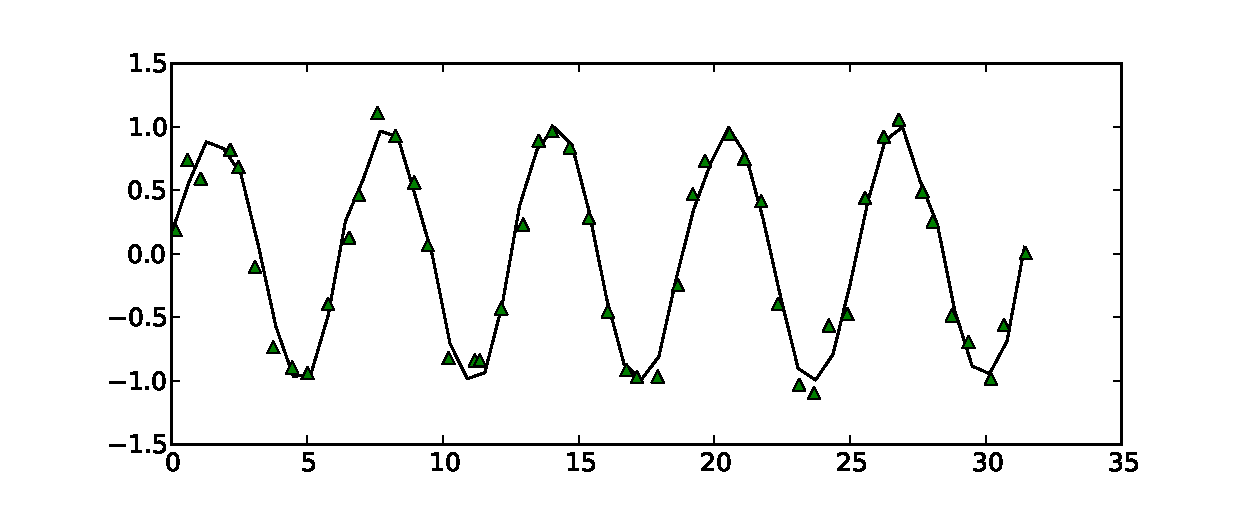
\includegraphics[scale=.4]{figures/interp1.eps}

%
%\subsection{Linear Interpolation}
%\begin{itemize}
%\item now we'll take the data and resample at even intervals by linear interpolation:
%\end{itemize}
%{\singlespacing \color{blue} \begin{verbatim}
%Xnew = numpy.arange(numpy.min(Xs),numpy.max(Xs),xinc)
%L=interp1d(Xs,Ys) # linear interpolation
%Ylin=L(Xnew)
%pylab.plot(Xnew,Ylin,'c', Xnew,Ylin,'c+')
%pylab.show()
%\end{verbatim}}
%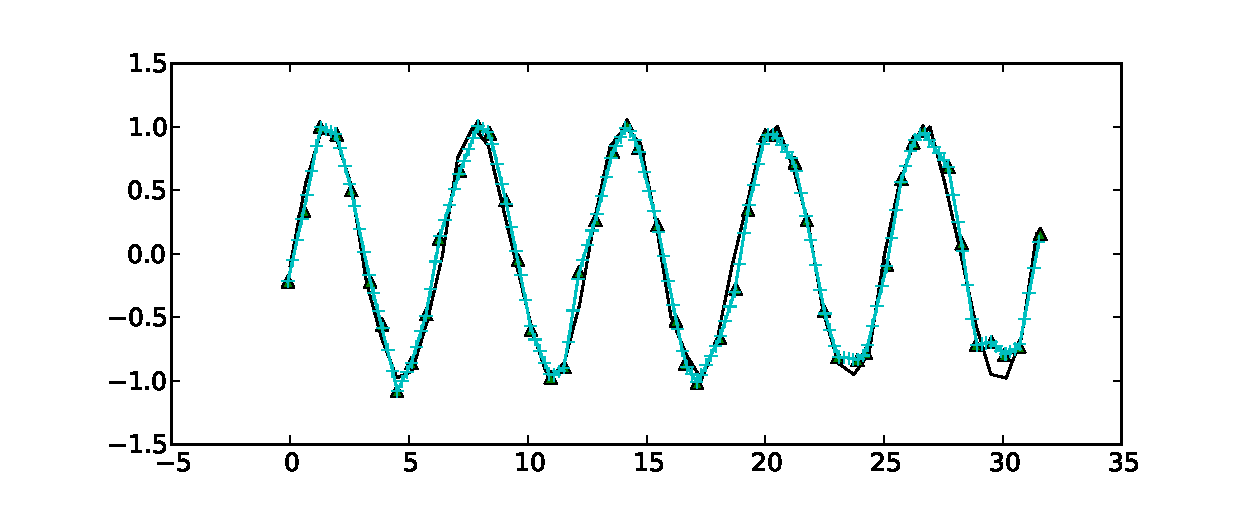
\includegraphics[scale=.4]{figures/interp2.eps}

%
%\subsection{Spline Interpolation}
%%%\vskip -.35in
%\begin{itemize}
%\item now let's try a simple spline interpolation
%\end{itemize}
%{\singlespacing \color{blue} \begin{verbatim}
%Xnew = numpy.arange(numpy.min(Xs),numpy.max(Xs),xinc)
%S=splrep(Xs,Ys) #spline representation
%Yspl=splev(Xnew,S) # evaluate the spline
%pylab.plot(Xnew,Yspl,'r', Xnew,Yspl,'r+')
%pylab.show()
%\end{verbatim}}
%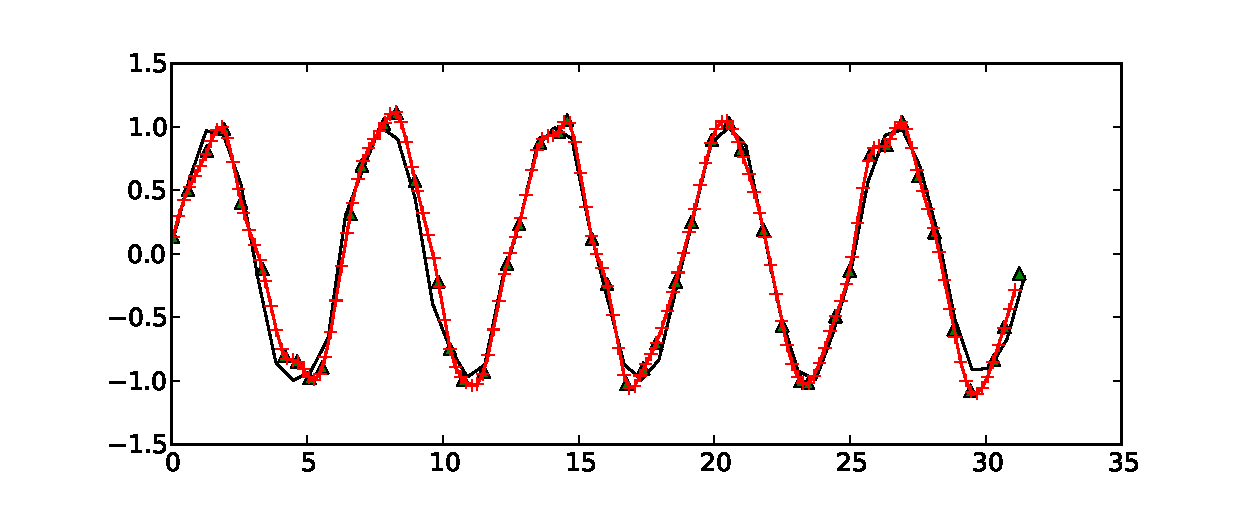
\includegraphics[scale=.4]{figures/spline.eps}

%Note: there are lot's of ways of doing splines so if you are serious about this, you should read the scipy documentation.



\section{Graphical User Interfaces - GUIs}

 Having introduced you to the joys of command lines, why now a lecture on GUIs?  
 GUIs work differently than all the other scripts we have been writing in that they don't just start at one end and proceed through to the end - the program flow can be controlled by the user.
GUIs let command line phobic people use your software.
They allows greater degree of interactivity with your data visualization.
They can streamline data analysis in an intuitive way.
And, they are fun.



Okay, how do I make  a GUI? 
 GUIs are composed of a number of things like text boxes, radio buttons, sliders, etc. called {\it widgets}.
 When the program starts, it first builds the GUI then waits for something to happen  (a menu to be selected or a mouse click or some data to be entered.... ) - a state called an {\it event loop}.  
There are a number of ways of creating GUIs in Python.  The oldest and most standard way is called {\color{blue}Tkinter} which is based on the even older UNIX language Tk.  
The newer {\color{blue}wxPython} has now reached some maturity and comes standard with the Enthought Python Distribution. see:


http://wiki.wxpython.org/Getting\%20Started

http://zetcode.com/wxpython/

and

http://wiki.wxpython.org/wxPython\%20by\%20Example

 It seems to be the way things are going, so we'll use wxPython in this class.







There are six essential parts to a wxPython GUI:

{\begin{tabular}{|l|l|}
\hline
import wx &Imports the necessary wxPython package\\
\hline
app = App()     &App() is a sub class of  wx.App \\
&app is an instance thereof\\
\hline
OnInit()  or  \_\_init\_\_()  function        &Specify what happens on initialization.\\
\hline
frame = wx.Frame()         &Frame is a class for the main windows\\
&frame is a particular window instance.\\
\hline
frame.Show()    &reveals the window - like pylab.show()\\
\hline
app.MainLoop()   &starts the progam\\
\hline
\end{tabular}

\noindent Here is a simple example that makes a window with an image in it:

%{\singlespacing \color{blue} \begin{verbatim}
%#!/usr/bin/env python   # shebang line
%import wx
%class App(wx.App):  
%    def OnInit(self):
%        image = wx.Image('tictactoe.jpg', wx.BITMAP_TYPE_JPEG) # makes an image object
%        self.frame = Frame(image) # makes the main window
%        self.frame.Show()
%        return True
%class Frame(wx.Frame): # describes the main window
%    def __init__(self, image, parent=None, id=-1,
%                 pos=wx.DefaultPosition, title='Hello, SIO 233 Class!'):
%        """Create a Frame instance and display image."""
%        temp = image.ConvertToBitmap()  # this and next line
%        size = temp.GetWidth(), temp.GetHeight() # prepares the image for display
%        wx.Frame.__init__(self, parent, id, title, pos, size) # initializes image
%        self.bmp = wx.StaticBitmap(parent=self, bitmap=temp) # displays image
%        self.SetClientSize(size) 
%        self.CreateStatusBar() # creates status bar
%        self.SetStatusText("Let's play TicTacToe!") # annotates status bar
%app = App() # makes application instance
%app.MainLoop() # starts the main loop event
%\end{verbatim}}

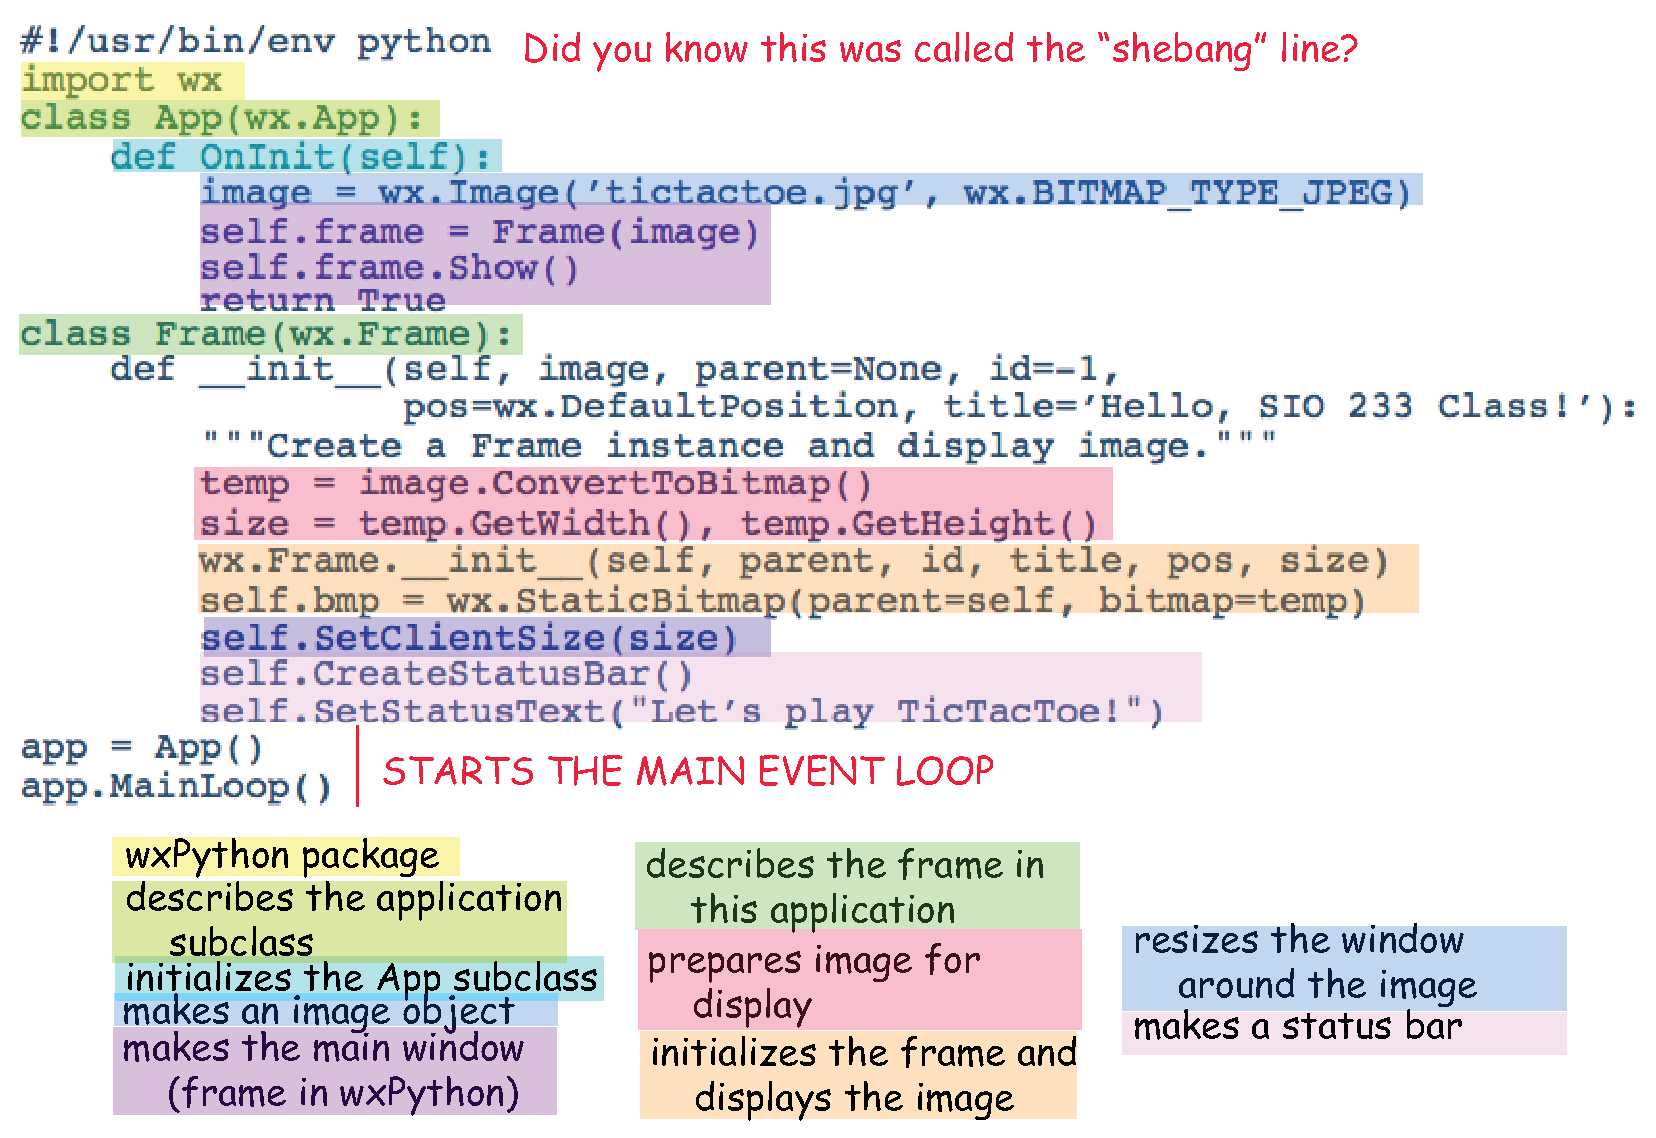
\includegraphics[width=6in]{figures/tictactoe1.eps} 

\noindent which makes this window:

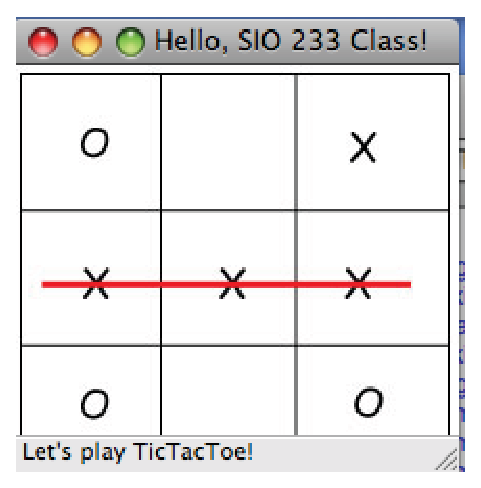
\includegraphics[width=1.75in]{figures/tictactoe2.eps} 




%
\eject
\centerline{Elements of a GUI:}

\begin{tabular}{|l|l|}
\hline
Widgets &Things you put on your GUI like text boxes, buttons, \\
& radio buttons, check boxes, pull down menus, etc.\\
& see figure below.\\
\hline
Events& Things that trigger actions like \\
& mouse movements and clicks, \\
& menu selections,  button clicks, etc.\\
\hline
 Dialogs and Messages & Pop up windows with information or action items.\\
  \hline
 Layout &   Setting up your GUI with a nice layout\\
  \hline
 Input and Output& Getting data in and out.\\
 \hline
\end{tabular}

\vskip 18pt
Here are some common GUI widgets:

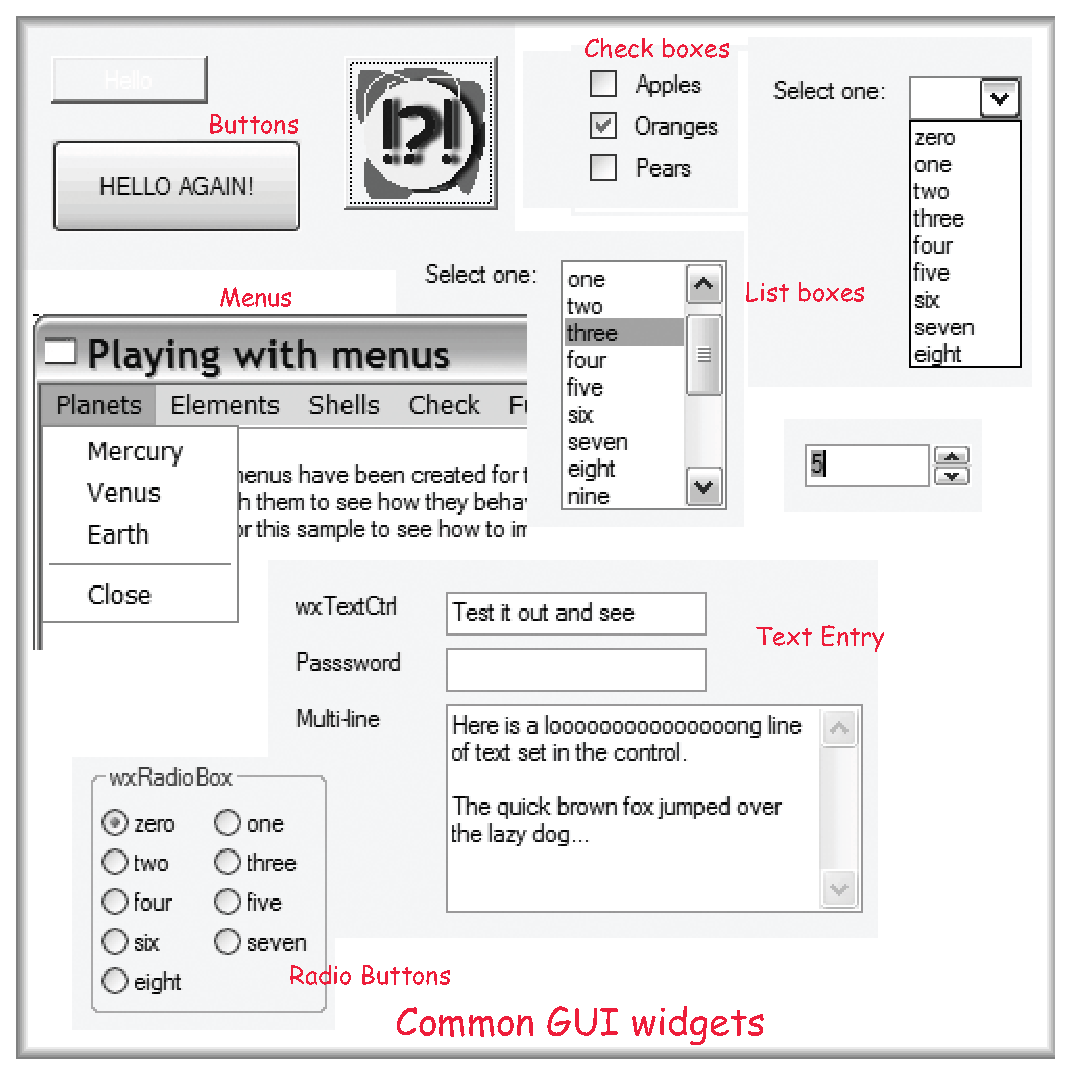
\includegraphics[width=4in]{figures/sampler.eps} 

From ``wxPython in Action'', by Rappin - a great intro to GUIs.

\noindent The example is for a simple editor  illustrating widgets, events, dialogs, and layout.

%{\singlespacing \color{blue} \begin{verbatim}
%#!/usr/bin/env python
%import wx
%class App(wx.App):
%    def OnInit(self):
%        self.frame=MyFrame(None,-1,'Editor')
%        self.frame.Show()
%        return True 
%class MyFrame(wx.Frame):
%    def __init__(self, parent,id,title):
%        wx.Frame.__init__(self, parent,id,title,(-1,-1),wx.Size(300,300))
%        panel=wx.Panel(self,-1)
%        box=wx.BoxSizer(wx.VERTICAL)
%        self.control=(wx.TextCtrl(panel,size=(300,250),style=wx.TE_MULTILINE))
%        box.Add(self.control)
%        button=wx.Button(panel, label="Quit")
%        button.Bind(wx.EVT_BUTTON, self.OnQuit)
%        box.Add(button)
%        panel.SetSizer(box)
%        self.Center()     
%    def OnQuit(self, event):
%        dlg = wx.MessageDialog(self,
%            "Do you really want to close this application?",
%            "Confirm Exit", wx.OK|wx.CANCEL|wx.ICON_QUESTION)
%        result = dlg.ShowModal()
%        dlg.Destroy()
%        if result == wx.ID_OK:
%            self.Destroy()
%app = App(False)
%app.MainLoop()
%\end{verbatim}}


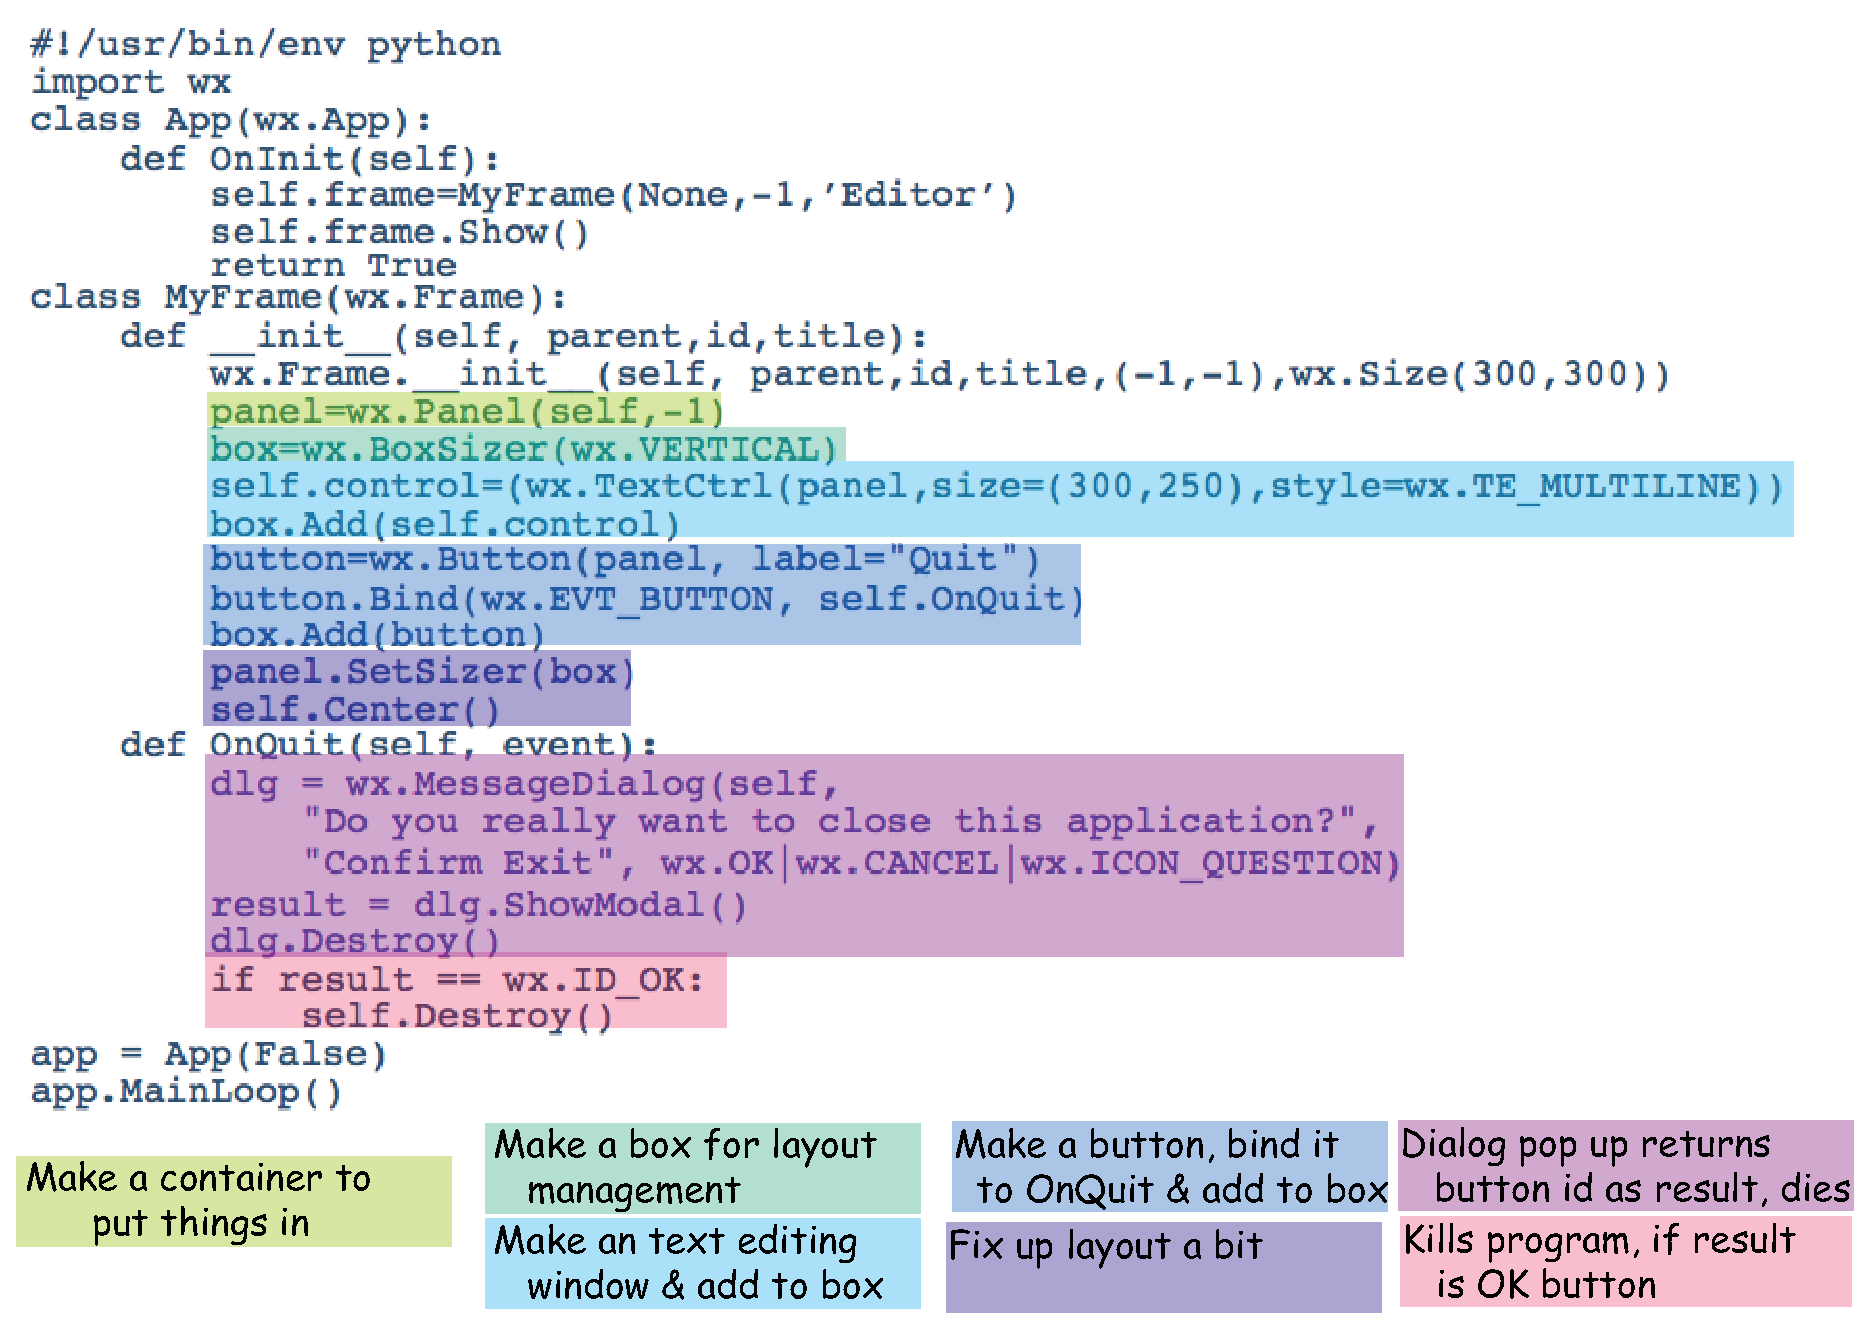
\includegraphics[width=6in]{figures/EditorButton.eps} 

\noindent which looks like this:

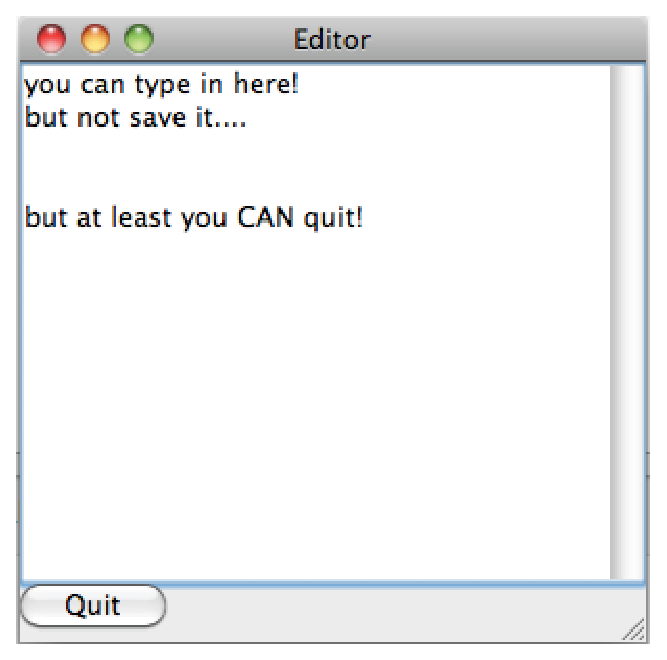
\includegraphics[width=3in]{figures/simple_editor.eps} 


\noindent Now let's add some file I/O:


%{\singlespacing \color{blue} \begin{verbatim}
%#!/usr/bin/env python
%import wx,os
%ID_OPEN,ID_EXIT=101,200
%class App(wx.App):
%    def OnInit(self):
%        self.frame=MyFrame(None,-1,'Editor')
%        self.frame.Show()
%        return True 
%class MyFrame(wx.Frame):
%    def __init__(self, parent,id,title):
%        wx.Frame.__init__(self, parent,id,title,(-1,-1),wx.Size(300,300))
%        panel=wx.Panel(self,-1)
%        box=wx.BoxSizer(wx.VERTICAL)
%        self.control=(wx.TextCtrl(panel,size=(300,250),style=wx.TE_MULTILINE))
%        box.Add(self.control)
%        panel.SetSizer(box)
%        self.Center()
%        filemenu = wx.Menu()
%        filemenu.Append(ID_OPEN, "&Open"," Open a file to edit")
%        filemenu.AppendSeparator()
%        filemenu.Append(ID_EXIT, "E&xit"," Quit program")
%        menubar = wx.MenuBar()
%        menubar.Append(filemenu, "&File")
%        self.SetMenuBar(menubar)
%        self.Bind(wx.EVT_MENU, self.OnOpen,id=ID_OPEN)
%        self.Bind(wx.EVT_MENU, self.OnQuit,id=ID_EXIT)
%        self.dirname=''
%    def OnQuit(self, event):
%        self.Destroy()
%    def OnOpen(self, event):
%        dlg = wx.FileDialog(self, "Choose a file", self.dirname, "", "*.*", wx.OPEN)
%        if dlg.ShowModal() == wx.ID_OK:
%            self.filename=dlg.GetFilename()
%            self.dirname=dlg.GetDirectory()
%            filehandle=open(os.path.join(self.dirname, self.filename),'rU')
%            self.control.SetValue(filehandle.read())
%            filehandle.close()
%            self.SetTitle("Editing ... "+self.filename)
%        dlg.Destroy()
%app = App(False)
%app.MainLoop()
%\end{verbatim}}

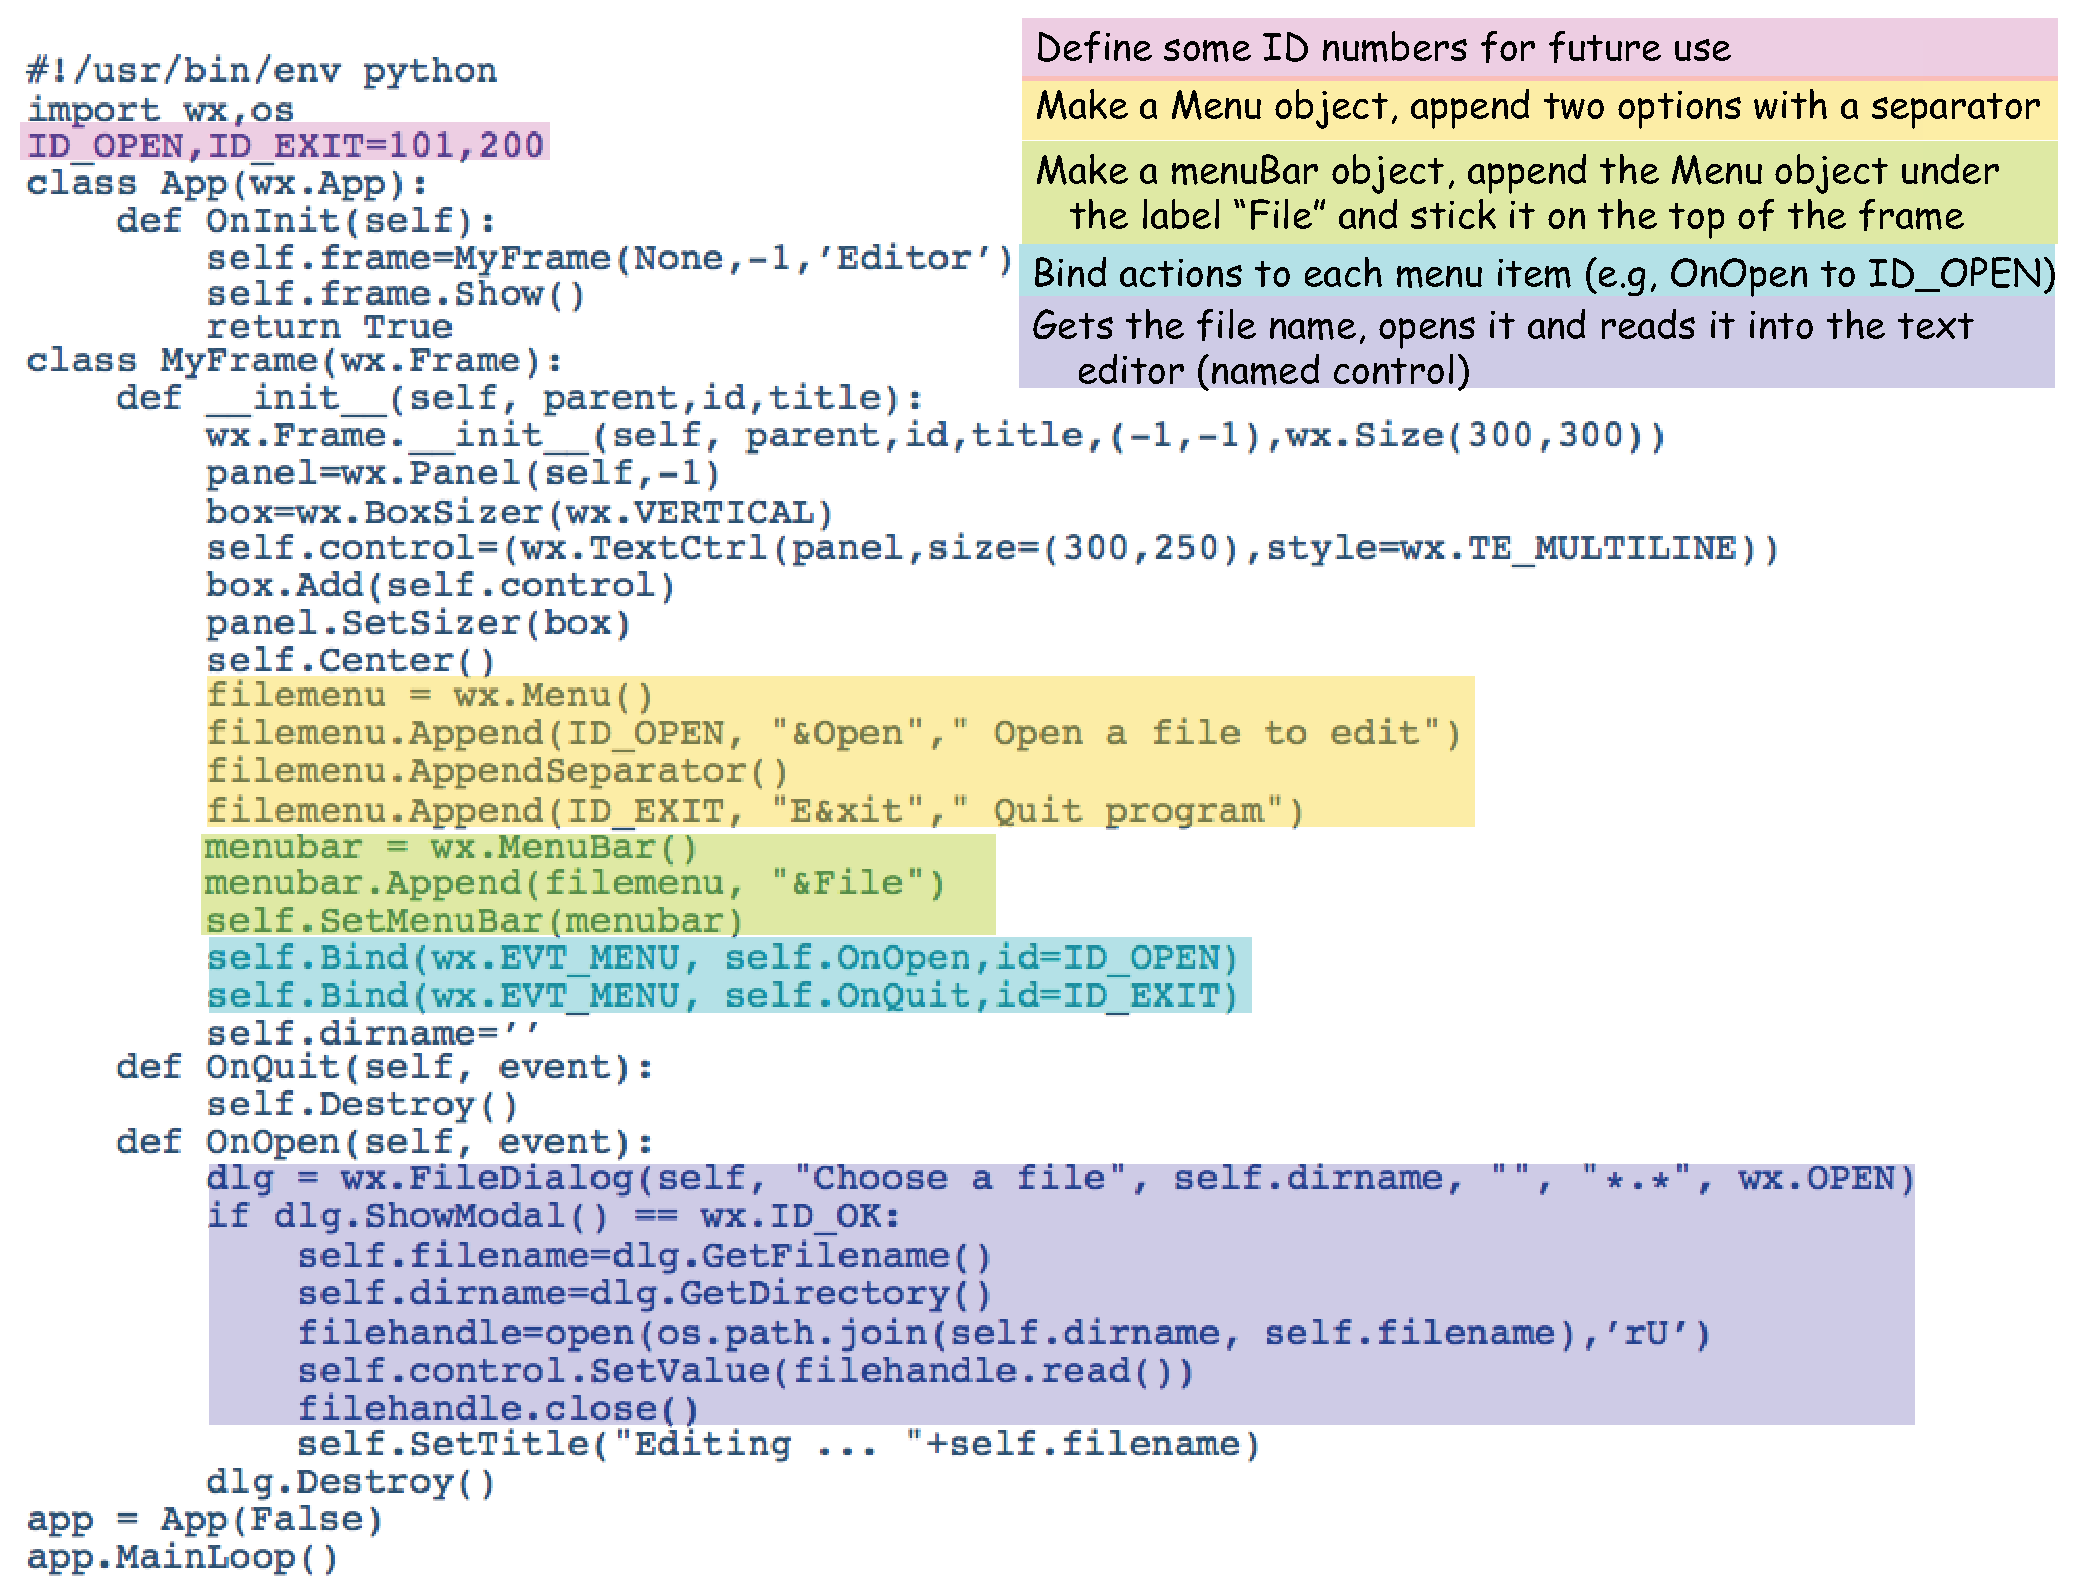
\includegraphics[width=5.5in]{figures/EditorMenu.eps} 

\noindent which creates a text box and a file menu.  You can open a file for editing (but saving it costs extra.)

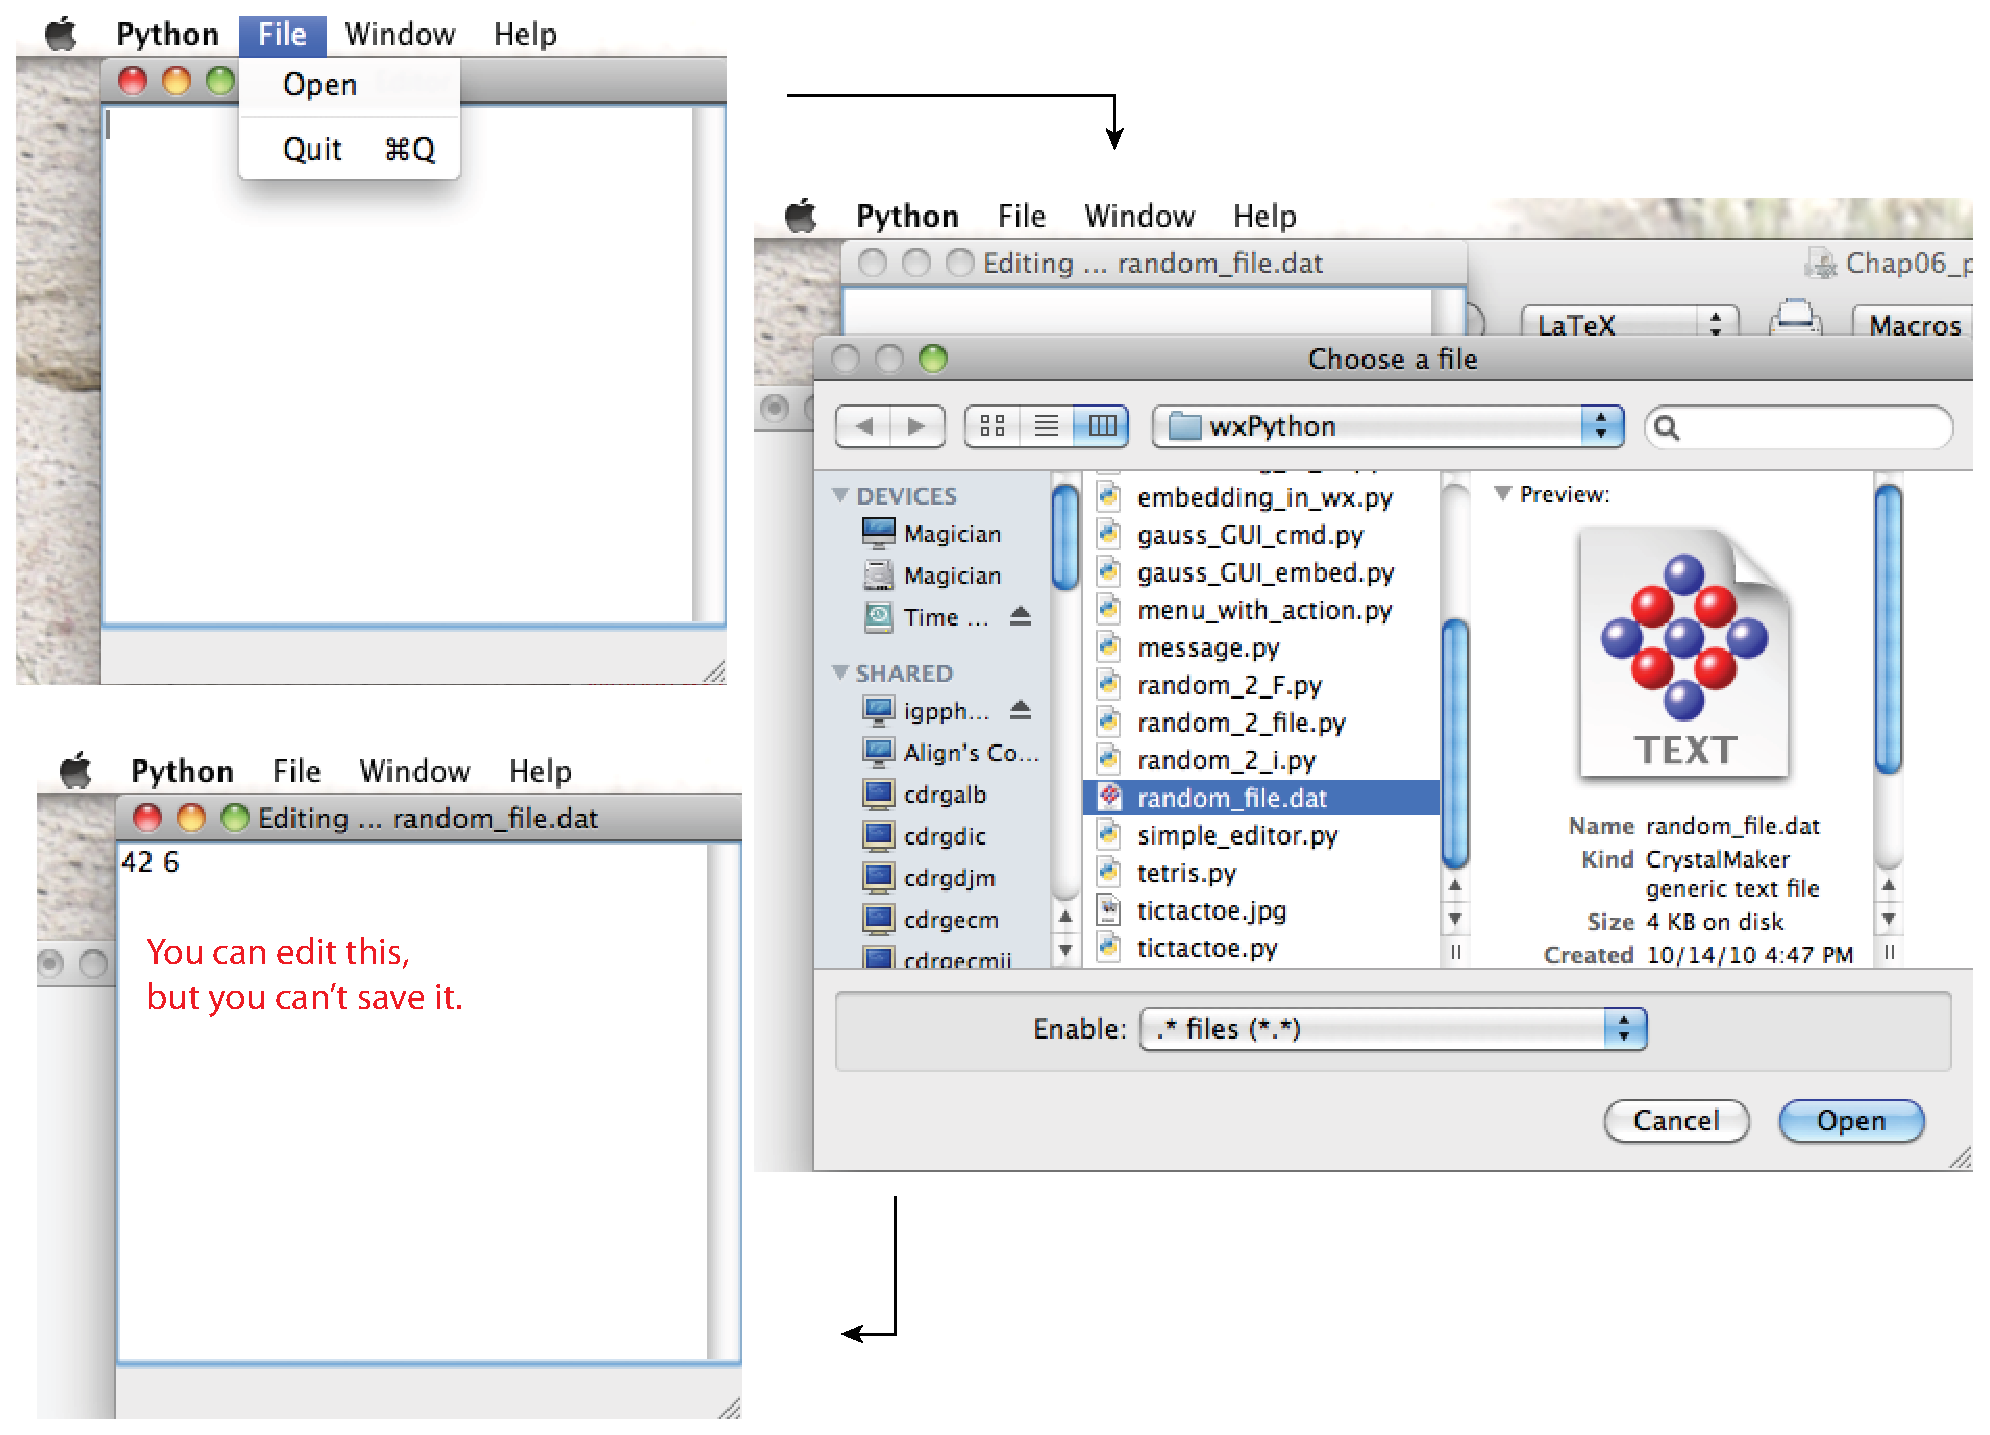
\includegraphics[width=5in]{figures/editor_menu.eps} 


\subsection{Interacting with plots}

In the section on statistics, I demonstrated a program to calculate gaussian data and plot them as a histogram.  
The mean and standard deviation were hardwired into the code.  
There are a bunch of ways we could make this program more customizable, some of which use GUIs:

\begin{enumerate}
\item  read in the mean and standard deviation using raw\_input() queries (annoying!)
\item   read them in from a file using a redirect $<$
\item   read them in as command line switches
\item   read them in from Entry boxes using a GUI, construct a command and running the program automatically through the command line as in the above ideas.  
\item  read them in from Entry boxes using a GUI, and call a method from within the GUI
\end{enumerate}

You should already know how to do the first three options from what you have already learned.  But here are a few examples for fun.  

{\bf \noindent Option 1) Program queries with raw\_input():}

{\singlespacing \color{blue} \begin{verbatim}
#!/usr/bin/env python
import matplotlib
matplotlib.use("TkAgg")
import pylab,sys
import exceptions # new module that allows error trapping!
from numpy import random
"""random_2_i"""
N,mu,sigma=500,10,2
pylab.ion()
fig=pylab.figure(1,figsize=(5,4))
while 1:
    Nums=[]
    try:   # executes unless error!
        mu=float(raw_input('Enter mean: '))
        sig=float(raw_input('Enter sigma: '))
        for i in range(N):
            Nums.append(random.normal(mu,sigma))
        pylab.hist(Nums,bins=20,facecolor='orange')
        pylab.title('Normal distribution')
        pylab.draw()
        ans=raw_input("Press return to continue, q to quit: ")
        if ans=='q': break
        pylab.clf() # clears figure so we can plot a new one
    except TypeError: # executes if there is a TypeError
       print 'Invalid entries, try again'
print 'Quitting'
\end{verbatim}}
}
 %  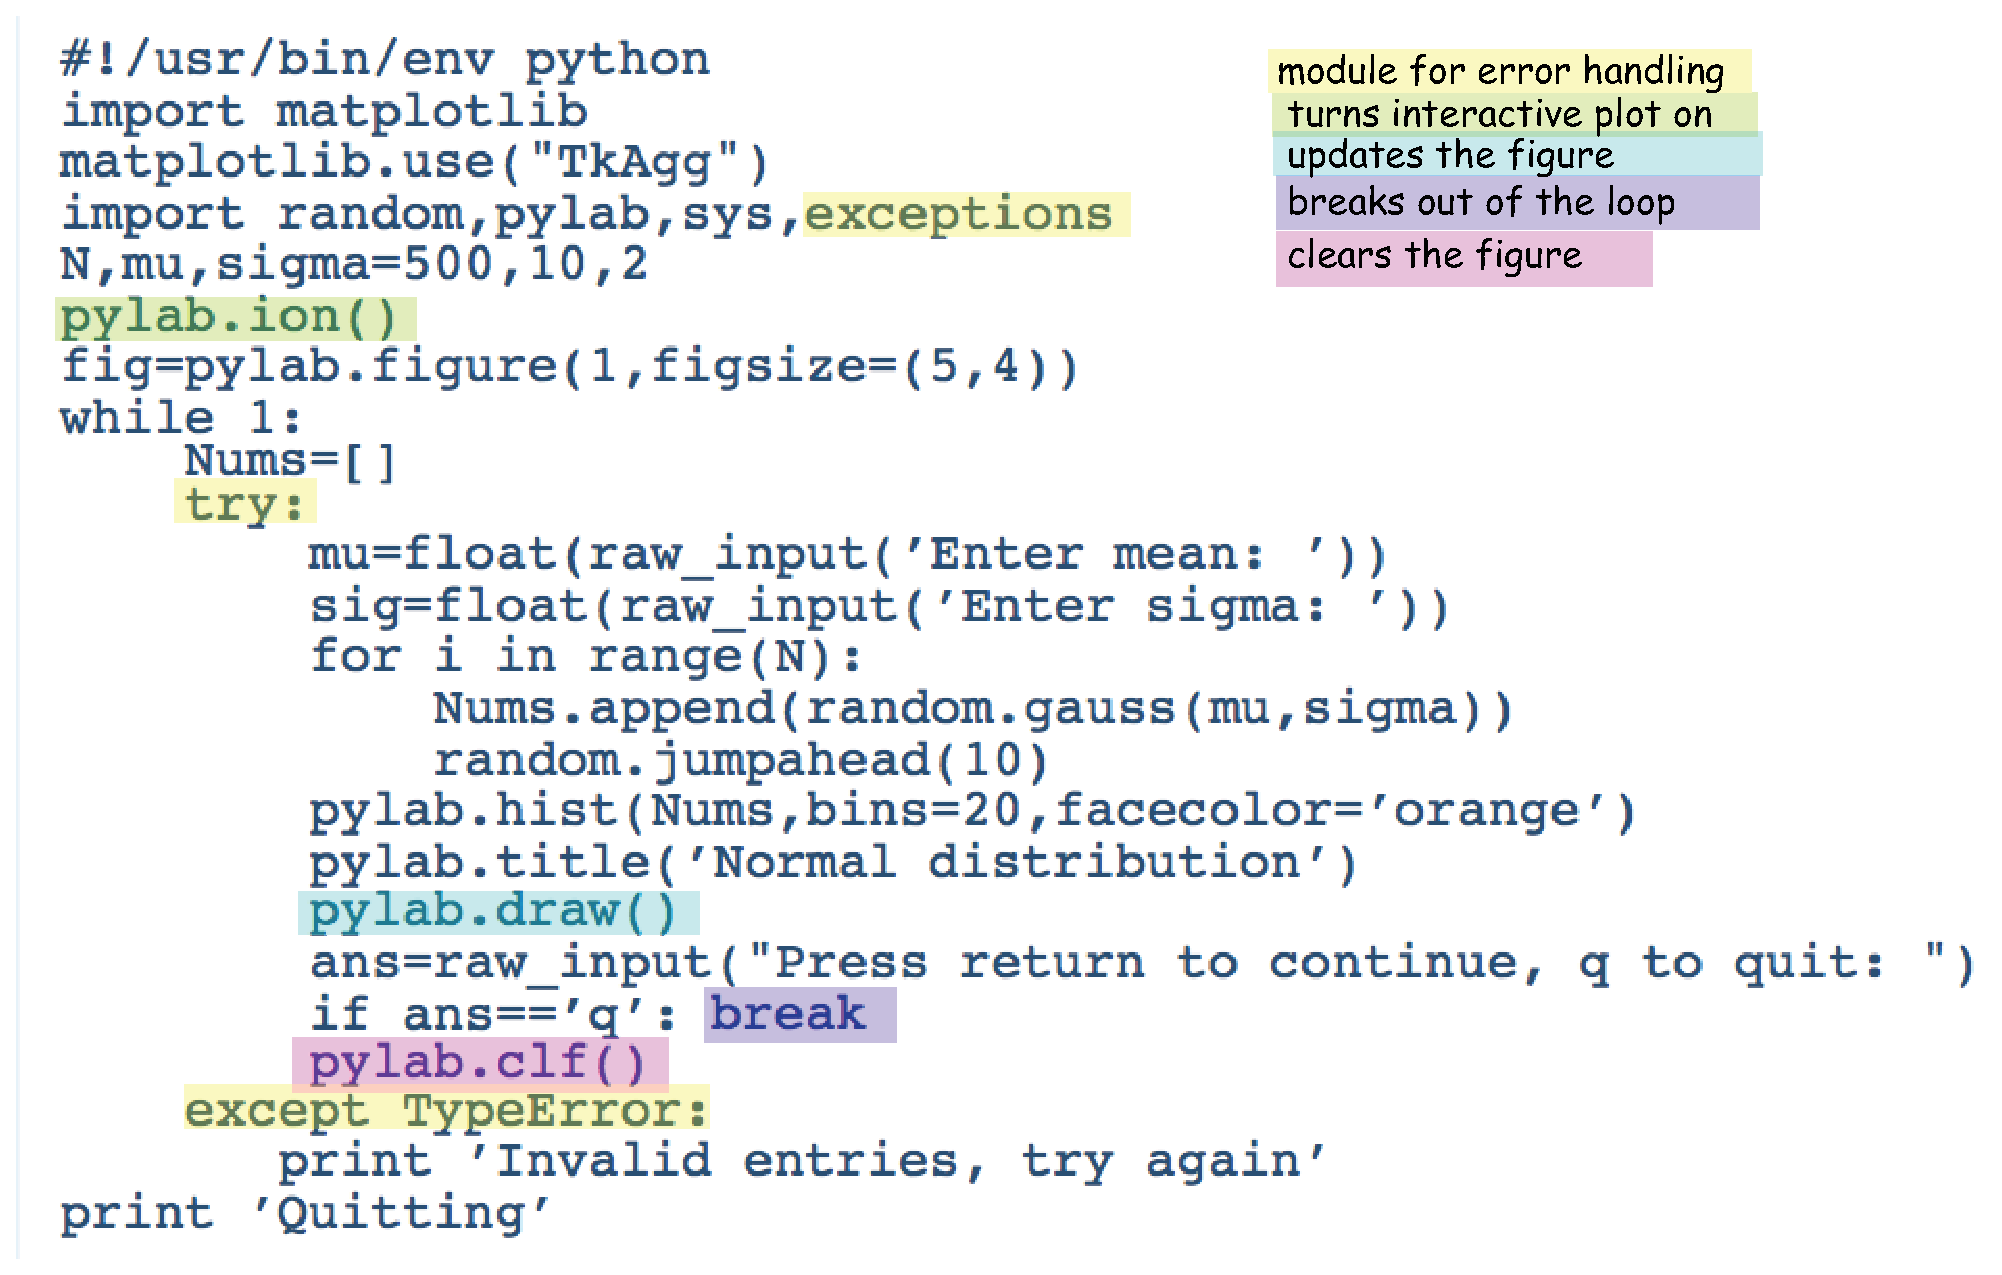
\includegraphics[width=4in]{figures/GaussInt.eps} 
 which produces this:   
 
 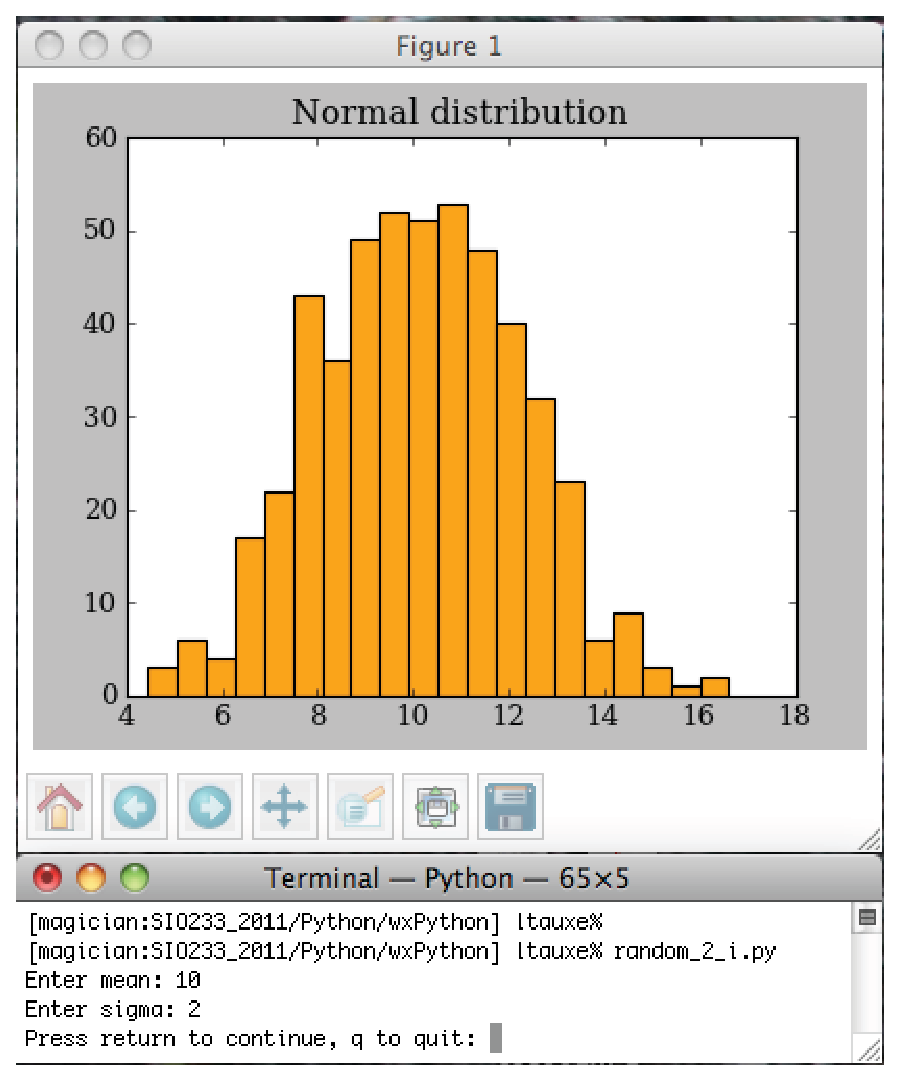
\includegraphics[width=4in]{figures/random_2_i.eps} 
   
   The program will keep updating the figure until you type 
  `q'.    There are two new things in this code snippet, which could come in handy:  1) the {\color{blue}pylab.clf()} command, which clears the figure and allows us to plot a new one and 2) error trapping with the module {\color{blue}exceptions}.   In this example, when you enter an invalid number, the error trap syntax:  
  {\singlespacing \color{blue} \begin{verbatim}
try:
    execute some code if no error happens
except:
    do this if you get an error - note you can specify the
    error type.
\end{verbatim}}

\noindent will give you a warning and then go back up to the top of the while loop.


  


{\bf \noindent Option 2) Read from standard input}


%\vskip -.35in
{\singlespacing \color{blue} \begin{verbatim}
#!/usr/bin/env python
import matplotlib
matplotlib.use("TkAgg")
import pylab,sys
from numpy import random
"""random\_2\_file.py"""
fig=pylab.figure(1,figsize=(5,4))
pylab.title('Normal distribution')
line=sys.stdin.readline()
N,Nums=500,[]
params=line.split()
mu,sigma=float(params[0]),float(params[1])
for i in range(N):
    Nums.append(random.normal(mu,sigma))
pylab.hist(Nums,bins=20,facecolor='orange')
pylab.show()
\end{verbatim}}
% 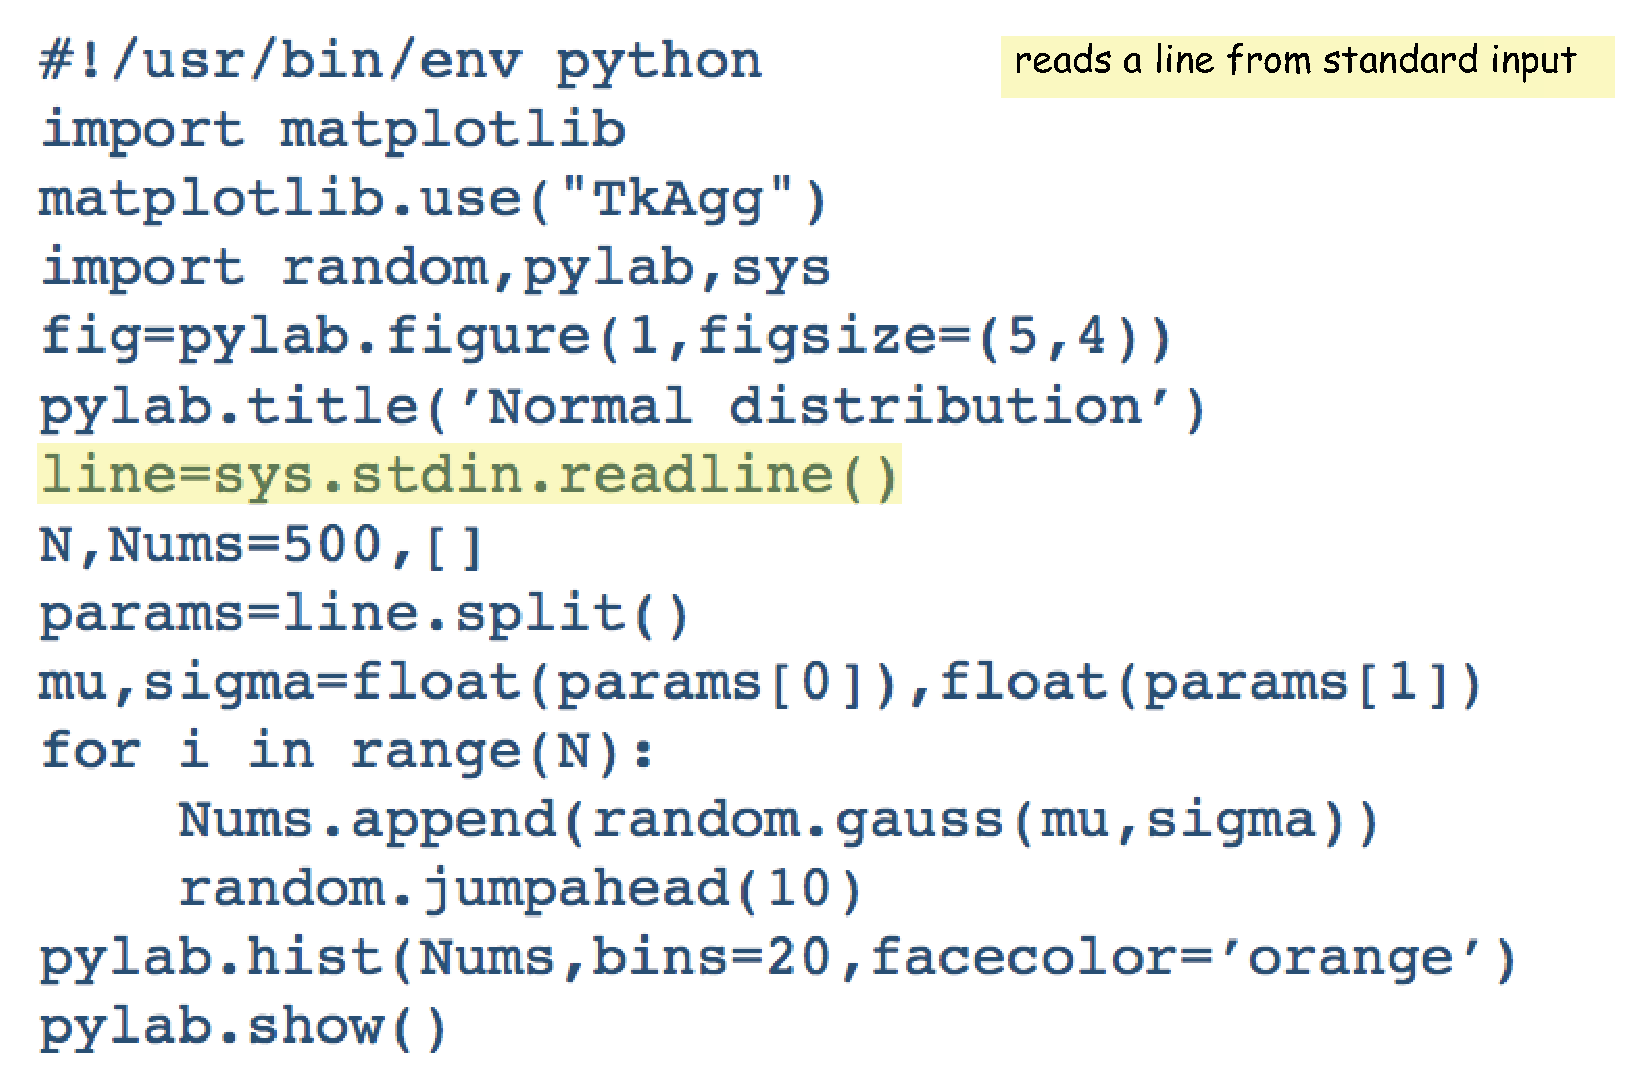
\includegraphics[width=4in]{figures/GaussStdin.eps}  

We can execute this program with a command like:

{\color{blue}\begin{verbatim}
% random_2_file.py < random_file.dat  
 \end{verbatim}}
   
   \noindent The file {\color{blue}random\_file.dat} contains the desired parameters.
   
   
 
 
 
{\bf \noindent Option 3)  Command line switch}

{\singlespacing \color{blue} \begin{verbatim}
#!/usr/bin/env python
import matplotlib
matplotlib.use("TkAgg")
import pylab,sys
from numpy import random
"""random\_2\_switch.py"""
N,mu,sigma=500,10,2
pylab.ion()
if '-mu' in sys.argv: mu=float(sys.argv[sys.argv.index('-mu')+1])
if '-sig' in sys.argv: sig=float(sys.argv[sys.argv.index('-sig')+1])
Nums=[]
for i in range(N):
    Nums.append(random.normal(mu,sigma))
pylab.hist(Nums,bins=20,facecolor='orange')
pylab.title('Normal distribution')
pylab.draw()
raw_input("Any key to quit")
\end{verbatim}}

This uses the already familiar use of command line switches and can be run with a command like:  


{\color{blue}\begin{verbatim}
% random_2_switch.py -mu 10 -sig 2
 \end{verbatim}}

{\bf \noindent Option 4)  Construct command line and run from within GUI:}
{\singlespacing \color{blue} \begin{verbatim}
#!/usr/bin/env python
import os,wx
""" gauss_GUI_cmd.py"""
ID_MEAN,ID_STD=101,102
class App(wx.App):
    def OnInit(self):
        self.frame=MyFrame(None,-1,'Gauss command line')
        self.frame.Center()
        self.frame.Show()
        return True 
class MyFrame(wx.Frame):
    def __init__(self, parent,id,title):
        wx.Frame.__init__(self,parent,id,title,(-1,-1),wx.Size(300,300))
        panel=wx.Panel(self,-1)
        self.mean_label=wx.StaticText(panel,-1,"   Mean",wx.DLG_PNT(panel,15,5))
        self.mean_entry=wx.TextCtrl(panel,ID_MEAN,"",wx.DLG_PNT(panel,40,5),\
           wx.DLG_SZE(panel,80,12))
        self.std_label=wx.StaticText(panel,-1,"   STD",wx.DLG_PNT(panel,15,20))
        self.std_entry=wx.TextCtrl(panel,ID_STD,"",wx.DLG_PNT(panel,40,20),
              wx.DLG_SZE(panel,80,12))
        button=wx.Button(panel,-1,"Plot",wx.DLG_PNT(panel,40,45),wx.DLG_SZE(panel,25,12))
        button.Bind(wx.EVT_BUTTON,self.PlotGauss)
    def PlotGauss(self,event):
        commandstring='random_2_switch.py -mu '+self.mean_entry.GetValue()
            +' -sig '+self.std_entry.GetValue()
        print 'running: ',commandstring
        os.system(commandstring)
app=App(False)
app.MainLoop()
\end{verbatim}}

\noindent And we get: 

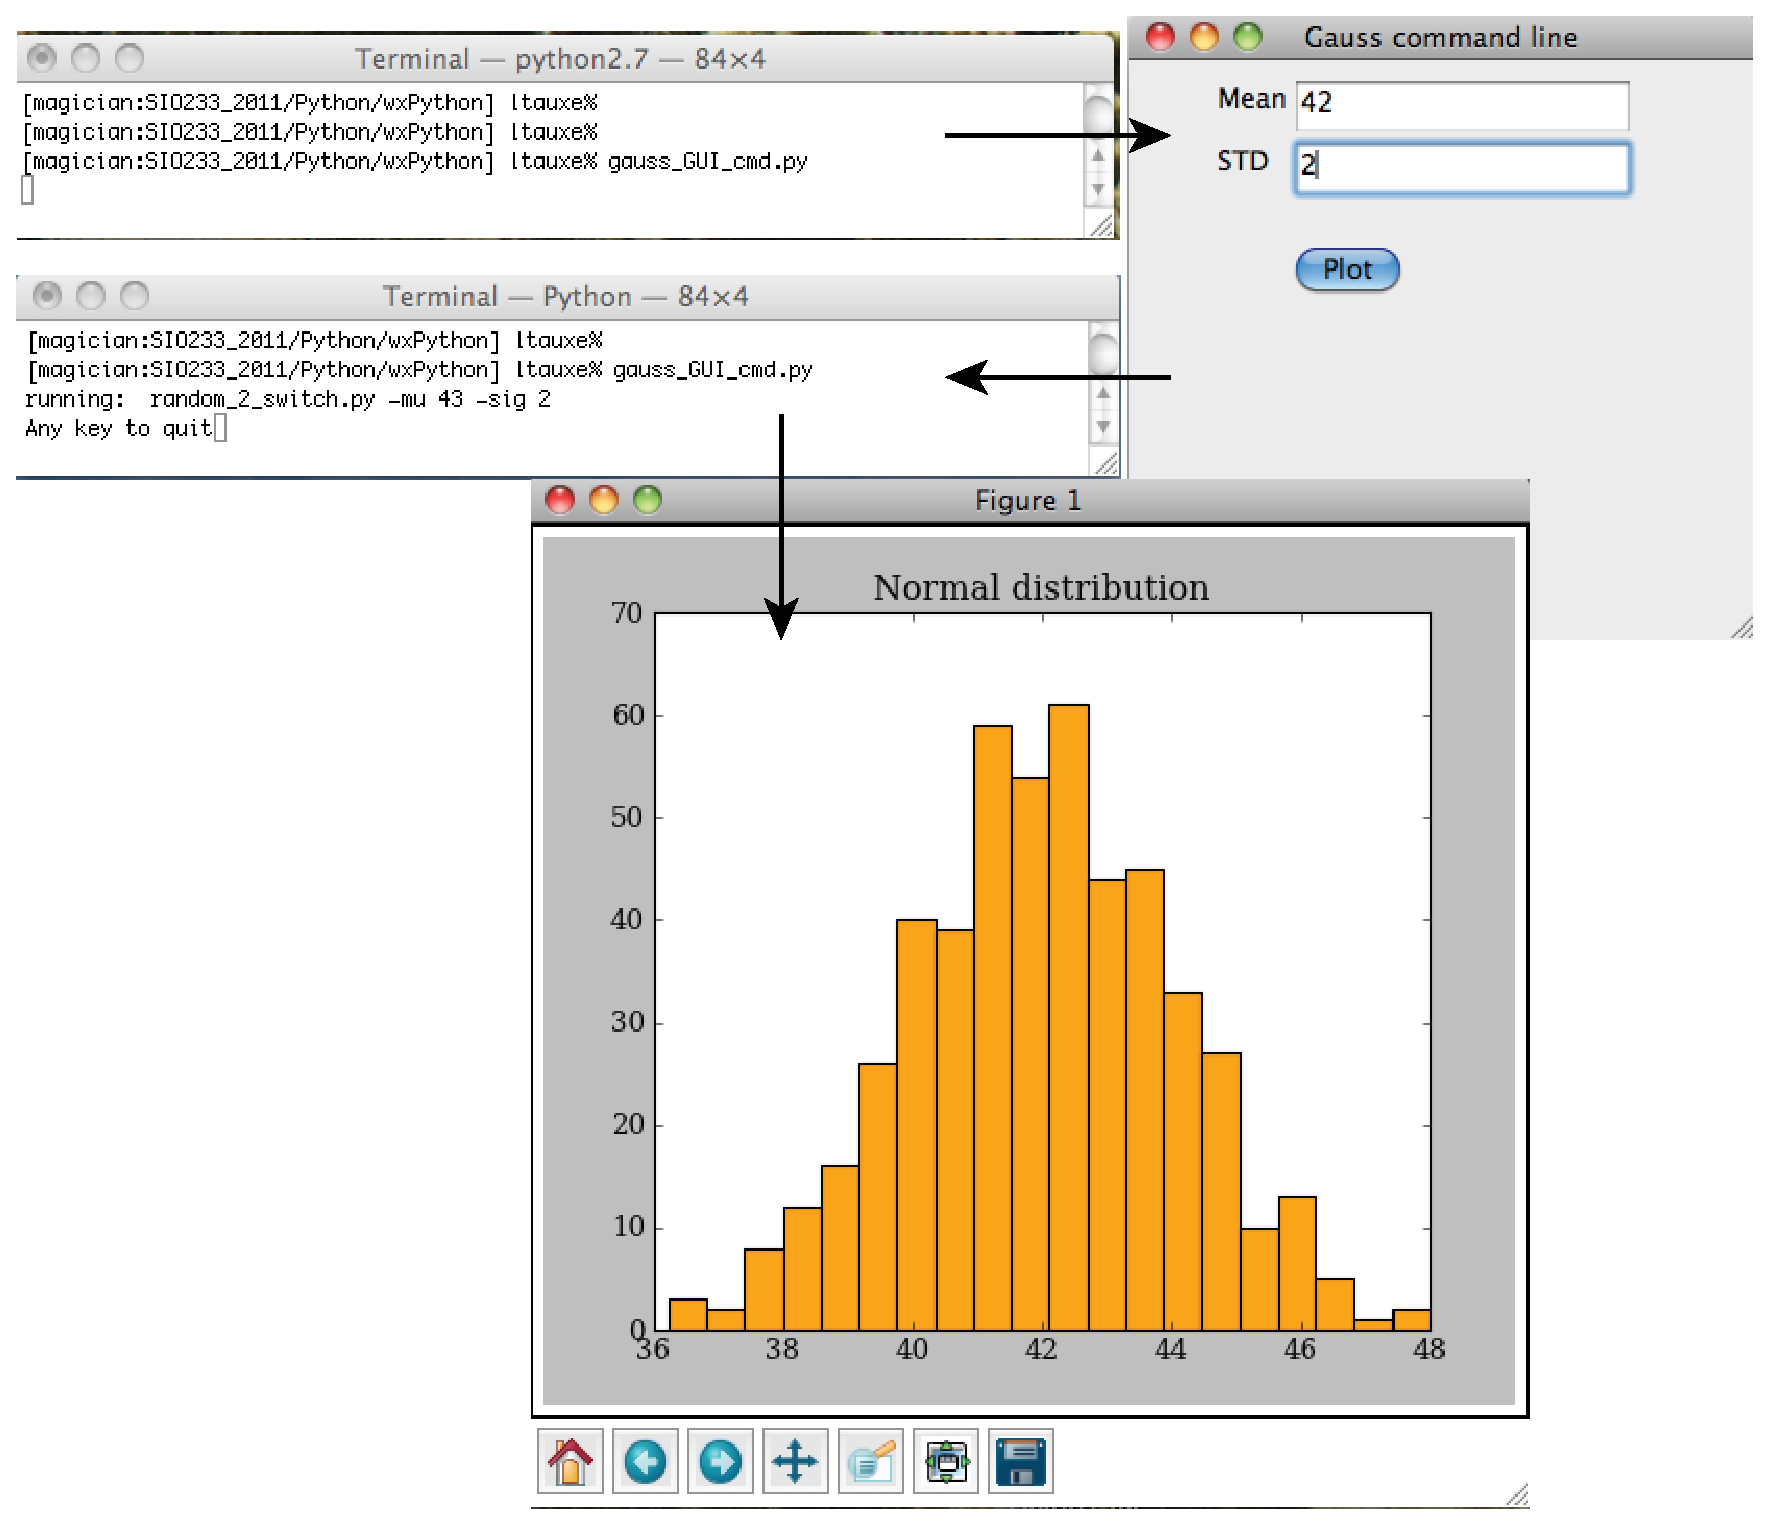
\includegraphics[width=5.25in]{figures/gauss_GUI_cmd.eps} 
 
 


{\bf \noindent Option 5) Embedding plot in GUI}

This is the most elegant option of all and makes us real GUI experts:  

\noindent  Basic Structure:

{\singlespacing \color{blue} \begin{verbatim}
#!/usr/bin/env python
import matplotlib; matplotlib.use('TkAgg')
from matplotlib.backends.backend_wx import FigureCanvasWx,\
     FigureManager, NavigationToolbar2Wx # import some matplotlib tools for  wxPython
import  numpy,pylab,wx
ID_MEAN,ID_STD,ID_PLOT=wx.NewId(),wx.NewId(),wx.NewId() # makes wxPython assign ids
class PlotFigure(wx.Frame): # initializes plot window
    def __init__(self):
        wx.Frame.__init__(self, None, -1, "matplotlib in wxFrame")
        
               HERE WE INITIALIZE SOME STUFF LIKE BUTTONS AND
                AND THE PLOT WINDOW
                
         def PlotGauss(self, event):
              
                 HERE WE DO THE PLOTTING
                 
         def OnQuit(self,event): # quits nicely
              self.Destroy()      
              
app = wx.PySimpleApp()  # a quick start for simple apps.  
frame = PlotFigure()  
frame.Show()
app.MainLoop()
\end{verbatim}}
% 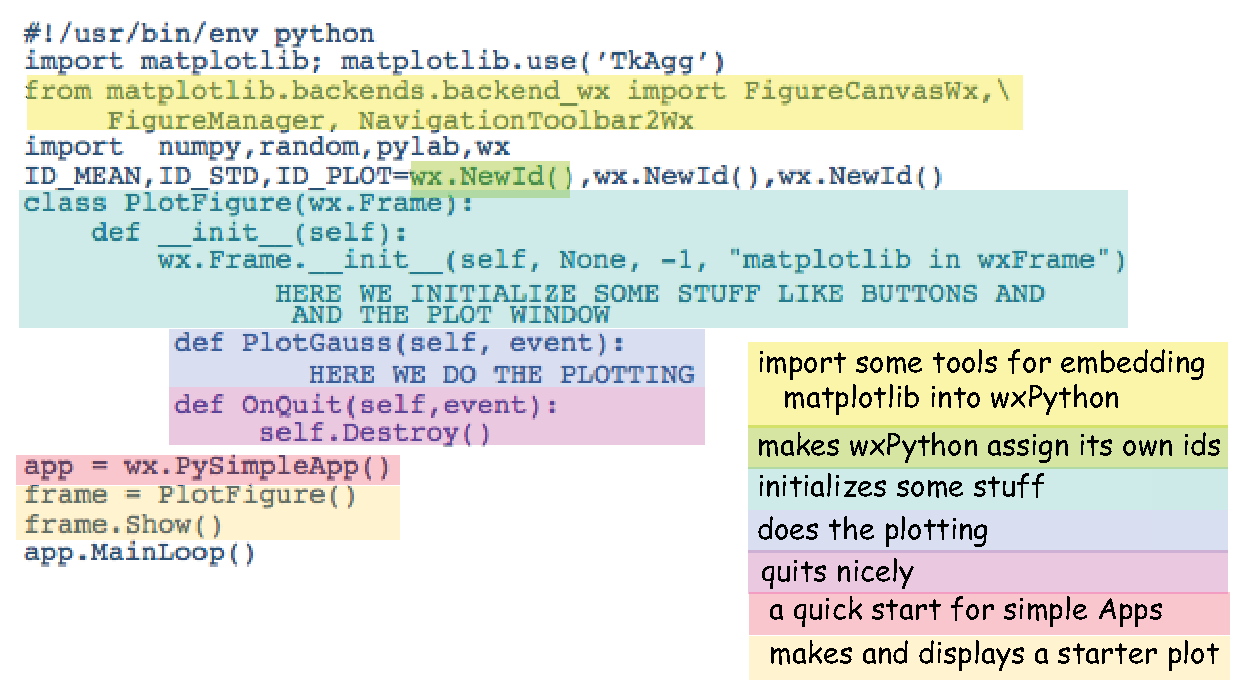
\includegraphics[width=5in]{figures/GaussEmbed1.eps} 



Let's take a closer look at the {\color{blue}PlotFigure} class.     This is where I design the basic GUI. 
 I want a plot window to stick my matplotlib figure. I want a toolbar under my figure.
 I want some text entry boxes for putting in the mean and standard deviation
 I want a button to trigger a new plot,  and I want a button to quit the program nicely.
 These all need to be laid out in a reasonable fashion.  
 
 So, first, I need to make some boxes to put things in.   Actually, I need two boxes for this:
 one to put all the text entry and plot widgets in
 and one to assemble everything nicely in.

To create the entry and plot widgets and putting them in a box I can use the following code: 

{\singlespacing \color{blue} \begin{verbatim}
box=wx.BoxSizer(wx.HORIZONTAL) # makes a box to put things in - horizontally
self.mean_label=wx.StaticText(self,-1,"   Mean") # makes a label
self.mean_entry=wx.TextCtrl(self,ID_MEAN,"") # makes a text entry box
self.mean_entry.SetValue('10.') # initializes the value to 10.
self.std_label=wx.StaticText(self,-1,"   STD") 
self.std_entry=wx.TextCtrl(self,ID_STD,"")
self.std_entry.SetValue('2.')
self.plotbutton=wx.Button(self,-1,"Plot") # makes a button labeled 'Plot'
self.plotbutton.Bind(wx.EVT_BUTTON,self.PlotGauss) # binds button to PlotGauss
self.quitbutton=wx.Button(self,-1,"Quit") # makes a button labeled 'Quit'
self.quitbutton.Bind(wx.EVT_BUTTON,self.OnQuit) # binds button to OnQuit 
box.Add(self.mean_label, 0, wx.GROW) # puts the 'mean' label into the box
box.Add(self.mean_entry, 0, wx.GROW) # puts in the mean text entry box
box.Add(self.std_label, 0, wx.GROW) # puts in the std label
box.Add(self.std_entry, 0, wx.GROW) # puts in the std text entry box
box.Add(self.plotbutton, 0, wx.GROW) # puts in the plot button
\end{verbatim}
}

% 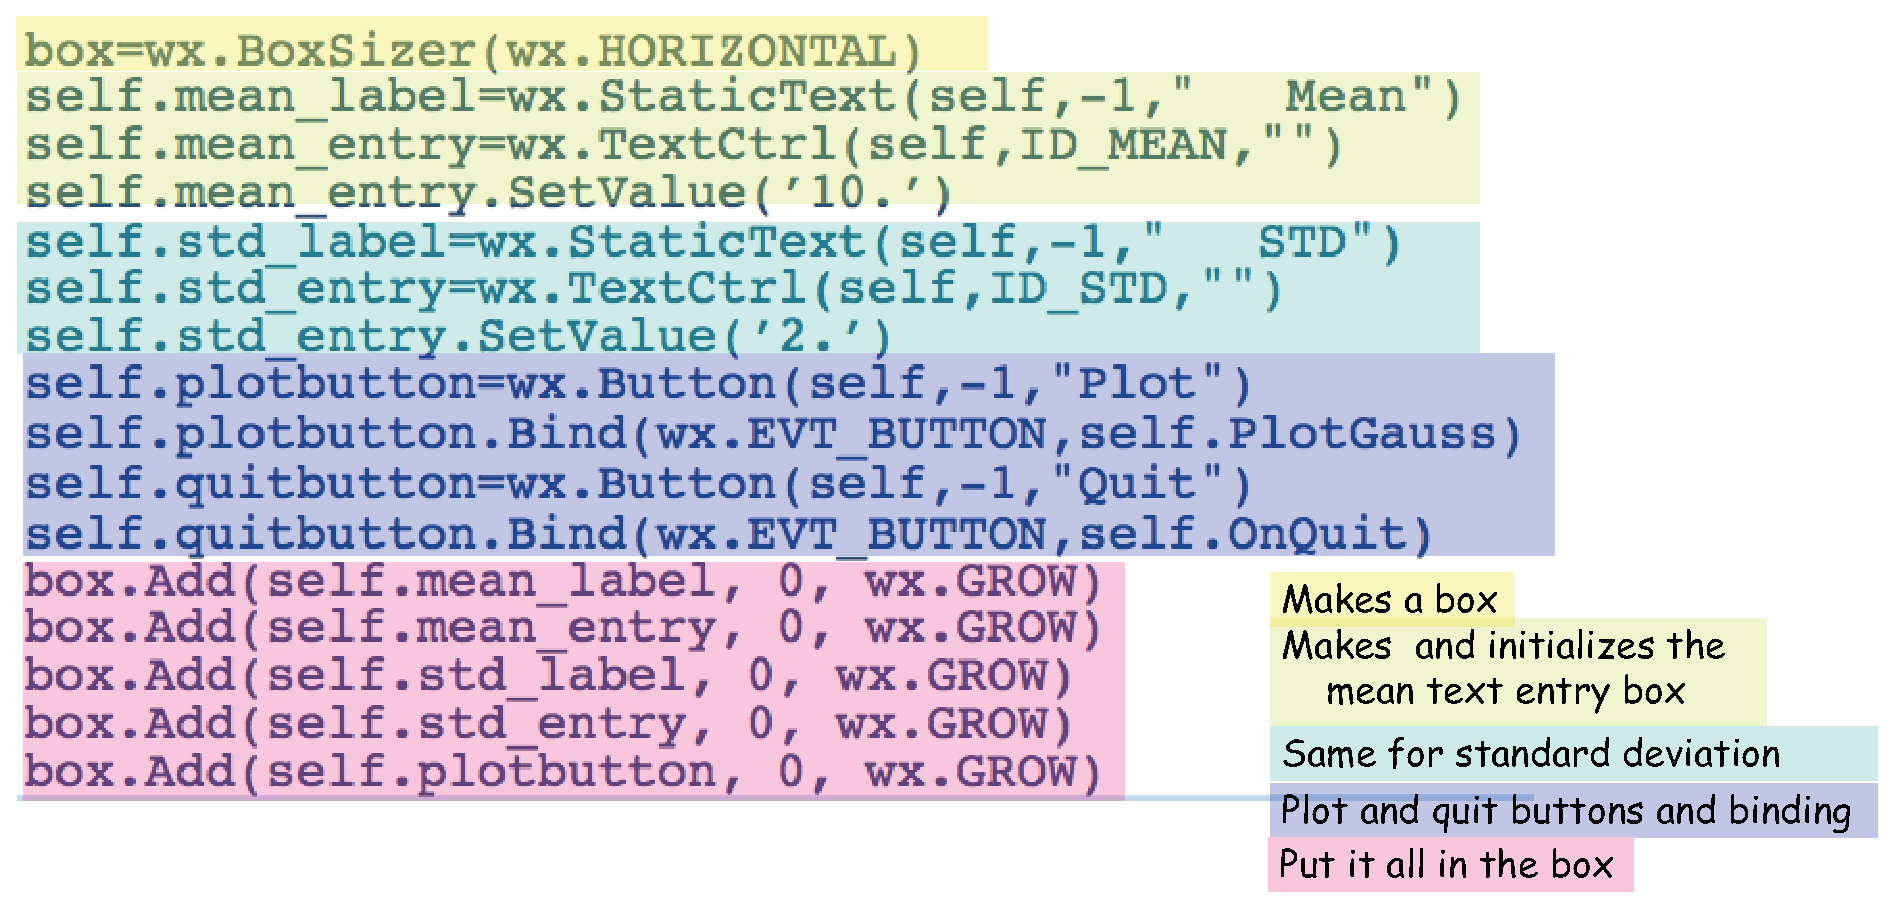
\includegraphics[width=6in]{figures/GaussEmbed2.eps} 


\noindent Now let's work on the  main box - here called `sizer':
%\vskip -.35in

{%\small  \baselineskip 0pt
{\singlespacing \color{blue} \begin{verbatim}
self.fig = pylab.figure(num=1,figsize=(5,4)) # make a figure instance
self.fig.add_subplot(111) # put a starter plot in it
self.PlotGauss(self) # make PlotGauss a method of this class
self.canvas = FigureCanvasWx(self, -1, self.fig) # make a canvas object, attach the figure
self.toolbar = NavigationToolbar2Wx(self.canvas) # make a toolbar
self.toolbar.Realize() # attach it to the canvas
tw, th = self.toolbar.GetSizeTuple() # get the size of the toolbar
fw, fh = self.canvas.GetSizeTuple() # get the size of the canvas
self.toolbar.SetSize(wx.Size(fw, th)) # set the width of the toolbar to the canvas
sizer = wx.BoxSizer(wx.VERTICAL) # make a box called sizer, things will add vertically
sizer.Add(self.canvas, 1, wx.LEFT|wx.TOP|wx.GROW) # put in the canvas
sizer.Add(box, 0, wx.GROW) # put in the widget box (with text entry boxes, etc.)
sizer.Add(self.quitbutton, 0, wx.GROW) # put in the quit button
sizer.Add(self.toolbar, 0, wx.GROW) # put in the toolbar
self.SetSizer(sizer) # resize things nicely
self.Fit() # make things fit in properly
\end{verbatim}}
}
% 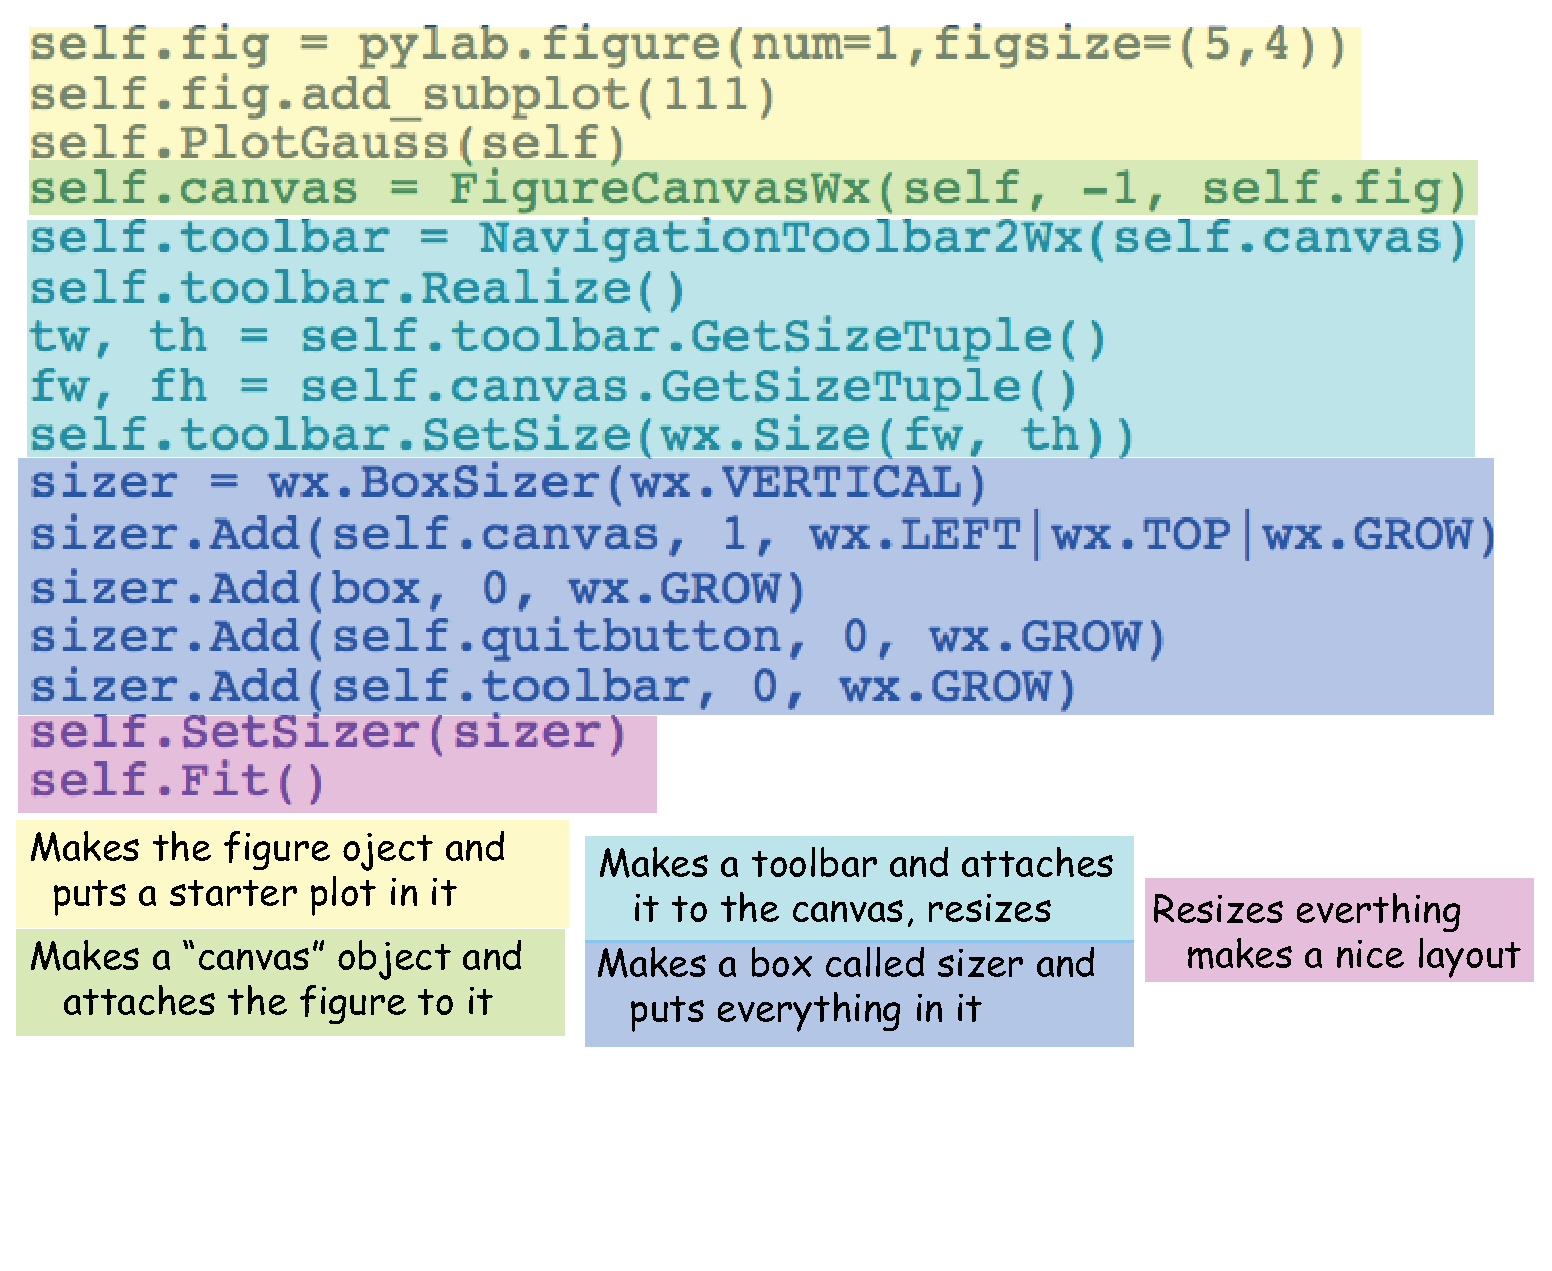
\includegraphics[width=6in]{figures/GaussEmbed3.eps} 


\noindent And finally  the plot function bit: 


{\singlespacing \color{blue} \begin{verbatim}
def PlotGauss(self, event):
    pylab.figure(num=1) # set the current figure to #1
    pylab.clf() # clear the current figure
    mu=float(self.mean_entry.GetValue()) # retrieve mu, sigma from their boxes
    sigma=float(self.std_entry.GetValue()) # and make them floats
    N,Nums=500,[]
    for i in range(N):
          Nums.append(random.normal(mu,sigma))
    pylab.hist(Nums,bins=20,facecolor='orange')
    self.canvas.draw() # redraw the plot window
    self.canvas.gui_repaint() # refresh the canvas frame with the new plot
\end{verbatim}}
}

% 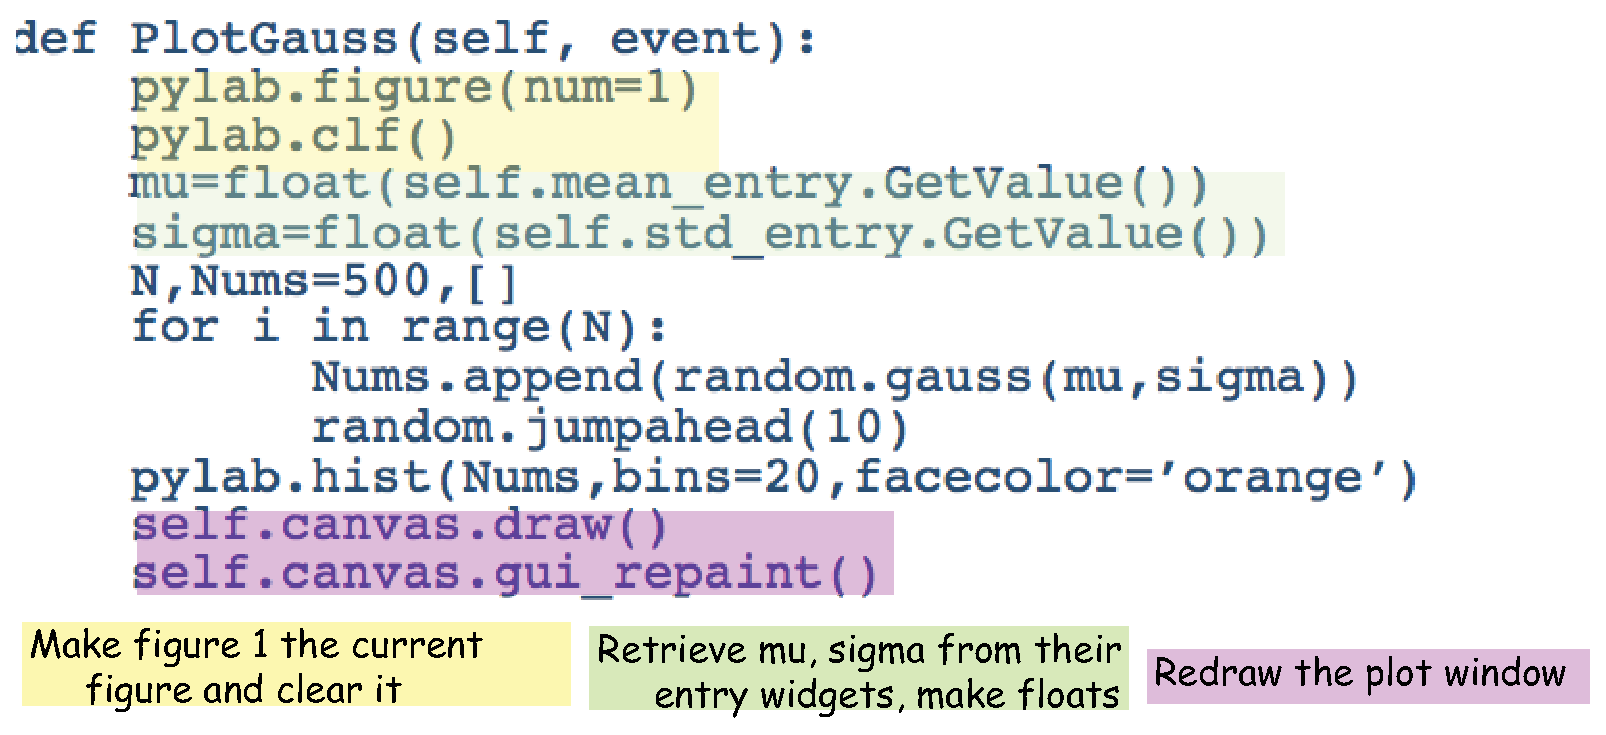
\includegraphics[width=6in]{figures/GaussEmbed4.eps} 


Putting it all together we have:
{\singlespacing \color{blue}\begin{verbatim}
#!/usr/bin/env python
import matplotlib; matplotlib.use('TkAgg')
from matplotlib.backends.backend_wx import FigureCanvasWx,\
     FigureManager, NavigationToolbar2Wx
import  numpy,pylab,wx
from numpy import random
"""Program gauss_GUI_embed.py"""
ID_MEAN,ID_STD,ID_PLOT=wx.NewId(),wx.NewId(),wx.NewId()
class PlotFigure(wx.Frame):
    def __init__(self):
        wx.Frame.__init__(self, None, -1, "matplotlib in wxFrame")
        self.fig = pylab.figure(num=1,figsize=(5,4))
        self.canvas = FigureCanvasWx(self, -1, self.fig)
        self.toolbar = NavigationToolbar2Wx(self.canvas)
        self.toolbar.Realize()
        tw, th = self.toolbar.GetSizeTuple()
        fw, fh = self.canvas.GetSizeTuple()
        self.toolbar.SetSize(wx.Size(fw, th))
        sizer = wx.BoxSizer(wx.VERTICAL)
        sizer.Add(self.canvas, 1, wx.LEFT|wx.TOP|wx.GROW)
        box=wx.BoxSizer(wx.HORIZONTAL)
        self.mean_label=wx.StaticText(self,-1,"   Mean")
        self.mean_entry=wx.TextCtrl(self,ID_MEAN,"")
        self.mean_entry.SetValue('10.')
        self.std_label=wx.StaticText(self,-1,"   STD")
        self.std_entry=wx.TextCtrl(self,ID_STD,"")
        self.std_entry.SetValue('2.')
        self.plotbutton=wx.Button(self,-1,"Plot")
        self.plotbutton.Bind(wx.EVT_BUTTON,self.PlotGauss)
        self.quitbutton=wx.Button(self,-1,"Quit")
        self.quitbutton.Bind(wx.EVT_BUTTON,self.OnQuit)
        box.Add(self.mean_label, 0, wx.GROW)
        box.Add(self.mean_entry, 0, wx.GROW)
        box.Add(self.std_label, 0, wx.GROW)
        box.Add(self.std_entry, 0, wx.GROW)
        box.Add(self.plotbutton, 0, wx.GROW)
        sizer.Add(box, 0, wx.GROW)
        sizer.Add(self.quitbutton, 0, wx.GROW)
        sizer.Add(self.toolbar, 0, wx.GROW)
        self.SetSizer(sizer)
        self.Fit()
        self.fig.add_subplot(111)
        self.PlotGauss(self)
    def PlotGauss(self, event):
        pylab.figure(num=1)
        pylab.clf()
        mu,sigma=float(self.mean_entry.GetValue()),float(self.std_entry.GetValue())
        N,Nums=500,[]
        for i in range(N):
            Nums.append(random.normal(mu,sigma))
        pylab.hist(Nums,bins=20,facecolor='orange')
        self.canvas.draw()
        self.canvas.gui_repaint()
    def OnQuit(self,event):
        self.Destroy()
app = wx.PySimpleApp()
frame = PlotFigure()
frame.Show()
app.MainLoop()
\end{verbatim}}


This gives a completed GUI that responds to the text entry and replots the histogram when the plot button is clicked. It also quits nicely when you click on `quit'.  

% 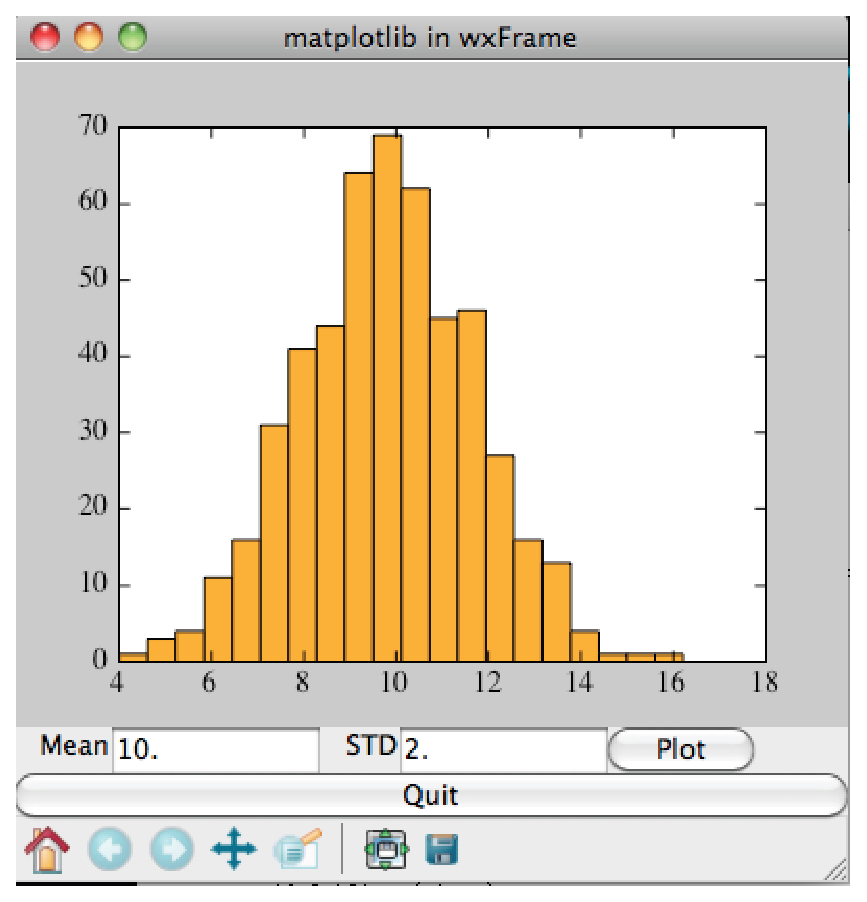
\includegraphics[width=3in]{figures/GaussEmbed5.eps} 
 
%
% 

%
%\section{Customizing matplotlib}
%%%\vskip -.35in
%\baselineskip 0pt
%\begin{itemize}
%\item Check if you have a directory '.matplotlib' in you home directory.  If not, make one.
%\item Download the file at:

%http://matplotlib.sourceforge.net/\_static/matplotlibrc

%and put it in a file called matplotlibrc in the directory .matplotlib

%
%\item  In there you will find a bunch of things that you can customize to make your 
%plotting more to your taste.
%\item In particular, if you are using 'TkAgg' as I do, you can specify that as your backend by changing the line:

%{\singlespacing \color{blue} \begin{verbatim}
%backend      : GTKAgg
%\end{verbatim}}

%to

%{\singlespacing \color{blue} \begin{verbatim}
%backend      : TkAgg
%\end{verbatim}}

%\item Then you never have to have the line {\it matplotlib.use('TkAgg')} in you code again.  There may be other back ends you like even better, but test them because they don't all work the same way.

%\item Look through the rest of the file and customize things like default line color or font as you like.
%\end{itemize}


\subsection{Event Handling in matplotlib}

%%\vskip -.35in

In the section on {\color{blue}matplotlib},  we learned about the {\color{blue}pylab} module. 
Behind the scenes,  {\color{blue}pylab} is an interface to three layers in {\color{blue}matplotlib}:  the {\color{blue}FigureCanvas} (the area onto which the figure gets drawn), the {\color{blue}Renderer} (the thing that does the drawing) and the {\color{blue}Artist} (controls the {\color{blue}Renderer} to paint on the {\color{blue}FigureCanvas}). 
Up to now, we  used {\color{blue}pylab}  handle the details for us. 
To take control of the plots (placement of figures, fonts, tickmarks, axes....) you need to know more about {\color{blue}Artist } containers ({\color{blue}Figure}, {\color{blue}Axis}, and {\color{blue}Axes}) and things that get drawn in them called ``primitives'' (lines, rectangles, text, images).
For a nice tutorial look in the matplotlib documentation:

http://matplotlib.sourceforge.net/users/artists.html\#artist-tutorial

\subsubsection{Artist}


 {\color{blue}Artist }  objects (like lines, tick marks, axes, text) are all configurable.
 When you use a command like {\color{blue}add\_axes} or {\color{blue}add\_subplot} you create an {\color{blue}Axes} instance. Remember how we made an  {\color{blue}Axes}  instance and called  {\color{blue} ax}?


{\singlespacing \color{blue} \begin{verbatim}
fig=pylab.figure()
ax=fig.add_subplot(111)
\end{verbatim}}

Every time you plot something on {\color{blue}fig} with,e.g.,  the {\color{blue}plot} command, you create an object of the Line2D class (yes even points). 
{\color{blue}pylab} keeps a record of each of these plot instances by  adding to a list associated with the {\color{blue}Axis} instance and retrieved by the method '{\color{blue}lines}' (e.g., {\color{blue}ax.lines} is the list of plotting calls on the  {\color{blue}Axes}  instance  {\color{blue}ax}).  
BTW:   This is how the {\color{blue}legend} commanworks, if you remember.
 So by identifying the line you want in the list, you can change its attributes (e.g., color, linewidth, linestyle or marker). I realize that was way more than you wanted to know right now, but we will need some idea of what {\color{blue}FigureCanvas} does in the following.   


\subsubsection{Line color}
%%\vskip -.35in
{\singlespacing \color{blue} \begin{verbatim}
#!/usr/bin/env python
import matplotlib
matplotlib.use("TkAgg")
import pylab, numpy
""" Program linecolor.py"""
pylab.ion() # makes plot interactive
fig=pylab.figure() # makes a figure instance
ax=fig.add_subplot(111) # Axes instance
t=numpy.arange(0,1,.01)
s=numpy.sin(2*numpy.pi*t)
c=numpy.cos(2*numpy.pi*t)
ax.plot(t,s,color='blue',lw=2) #Line2D instance
ax.plot(t,c,color='magenta',lw=2)
pylab.draw()
print ax.lines # prints all your plot instances
print 'last line color: ',ax.lines[-1].get_color()
raw_input("Any key to change last line to red ")
ax.lines[-1].set_color('red') # sets last line to red
pylab.draw()
raw_input()
\end{verbatim}}



\subsubsection{Mouse events}

Earlier, we learned how to make GUIs using {\color{blue}wxPython} and even managed to embed a {\color{blue}matplotlib} figure into a {\color{blue}wxPython Frame}.  But we couldn't interact with the plot directly, say by clicking on an individual box in the tictactoe example and have the program place an 'X' or an 'O' there.  
To do this, we need the program to recognize key or mouse events and return these to the program.
 In {\color{blue}wxPython} we had events ({\color{blue} EVT\_BUTTON}) which were connected to callback functions (like {\color{blue} OnQuit}) using the method {\color{blue}BIND}.  
In {\color{blue}matplotlib}  we have a similar event  {\color{blue}'button\_press\_event' } which can be connected to a function (e.g., {\color{blue}onclick}) using the {\color{blue}FigureCanvas} method {\color{blue} mpl\_connect}, e.g.:

{%%\tiny \baselineskip 0pt
{\singlespacing \color{blue} \begin{verbatim}
 fig.canvas.mpl_connect('button_press_event', \
     onclick)
 \end{verbatim}}
 }
 
 
 Mouse events are the most common type of interaction with plots.
We can use them to identify data points, say in a digitizer, or to flag them as bad, or pick them as special (e.g., P wave arrival, stratigraphic tie point, start or end point for a calculation)
matplotlib supports several mouse events:

%%\vskip 12pt
\begin{tabular}{l|l}
\hline
Event Name & Description\\
 'button\_press\_event':  &  mouse button pressed\\
 'button\_release\_event'&mouse button is released\\
 'motion\_notify\_event'&mouse action\\
 'scroll\_event' & mouse scroll wheel is rolled\\
 'pick\_event'& an Artist object is selected\\
 \hline
 \end{tabular}
 
Here is an example of a button press event:


 %%\vskip -.35in
{\singlespacing \color{blue} \begin{verbatim}
#!/usr/bin/env python
""" Program onclick.py"""
import matplotlib, numpy
matplotlib.use("TkAgg")
import pylab
from matplotlib.backend_bases import FigureCanvasBase # imports canvas tools
pylab.ion()  
fig=pylab.figure()
ax=fig.add_subplot(111)
data=numpy.random.rand(10) # get 10 random numbers
ax.plot(data)
ax.plot(data,'ro')
pylab.draw()
def onclick(event):
    print 'button=%d, x=%d, y=%d, xdata=%f,\
        ydata=%f'%(event.button, event.x, event.y, \
          event.xdata, event.ydata)
cid=fig.canvas.mpl_connect('button_press_event',\
    onclick) # connect the button press to the function onclick
raw_input()  #pauses the program
\end{verbatim}}


You could combine this with the editor  we wrote before to make a digitizer! 


In the last example, we just identified the location of the mouse click, but didn't identify any particular plot object.   In principle, each object (line, text, rectangle, axes) could be picked.  
There is a catch however.   When you create the object, you have to do these things too:

\begin{enumerate}
\item set the `picker' to True (and usually some floating point tolerance).
\item connect the `pick\_event' to some action
\item define the action.
\end{enumerate}

Consider the following program:   

 {\singlespacing \color{blue} \begin{verbatim}
#!/usr/bin/env python
import matplotlib; matplotlib.use("TkAgg")
import pylab,numpy
class LineColor: 
    """connects the picker to an Artist Line2D object and changes line color"""
    def __init__(self,line):
        self.line=line
        self.connect=\
           self.line.figure.canvas.mpl_connect(\
            'pick_event',self.on_pick)  
    def on_pick(self,event): # finds right line
        if event.artist!=self.line: return 
        self.line.set_color('red') # makes red
        self.line.set_linewidth(2) # makes fatter
        self.line.figure.canvas.draw() # redraws line
def main():
    """
    Program clickme.py
    Plots some lines that are clickable, connects them to the LineColor action.
    """
    fig=pylab.figure()
    ax=fig.add_subplot(111)
    t=numpy.arange(0,1,.01)
    s=numpy.sin(2*numpy.pi*t)
    ax.plot(t,s,color='blue',picker=True)
    ax.plot(t+.25*numpy.pi,s,color='magenta',picker=True)
    ax.plot(t+.5*numpy.pi,s,color='cyan',picker=True)
    lines=[]  # makes a list to store clickable line objects
    for line in ax.lines:  # steps through list of plot objects
        ln=LineColor(line) # make the line a LineColor objects
        lines.append(ln) # stores in the list
    pylab.show()
main()
\end{verbatim}}
 
\noindent  The class {\color{blue}LineColor} is the action that happens when a plot object gets clicked on. On initialization, it connects the click action to the function {\color{blue}on\_pick} which turns the object red and fattens it up a bit.   The main program draws some lines.  Each plot instance gets stored in the list ax.lines.  Then the objects in ax.lines get turned into clickable LineColor objects.   When you click on a line, it turns red and fattens up a bit.  

Your final is to do a tic-tac-toe program, and it would be fun to make it work inside a GUI.  To get you most of the way there,  I wrote  a  really silly   Tic-Tac-Toe program.  It is not a GUI, just a clickable matplotlib window:   

{\singlespacing \color{blue}\begin{verbatim}
#!/usr/bin/env python
import matplotlib
matplotlib.use("TkAgg")
import pylab
import numpy,sys,exceptions
from numpy import random
def finish(who,xline,yline):
    """ Check who won"""
    if len(xline)>0:
        if who==0:     # player wins
            pylab.plot(xline,yline,'r-')
            print 'you have won!'
        else: # computer wins
            pylab.plot(xline,yline,'g-')
            raw_input('you have lost to a stupid computer!')
        pylab.draw()
        cid = fig.canvas.mpl_connect('button_press_event', quit) # quit on mouse click
        print 'click anywhere on plot to quit'
def quit(event): # graceful exit
    sys.exit() 


def winner(who,myboxes):  
    """ checks to see if boxes selected have won """
    # check for diagonals first 
    if '11' in myboxes and '22' in myboxes and '33' in myboxes: \
          finish(who, [.5,2.5],[.5,2.5])
    if '13' in myboxes and '22' in myboxes and '31' in myboxes: \
         finish(who, [.5,2.5],[2.5,.5])
    # check for rows)
    if '11' in myboxes and '21' in myboxes and '31' in myboxes: \
         finish(who, [.5,2.5],[.5,.5])
    if '12' in myboxes and '22' in myboxes and '32' in myboxes: \
         finish(who, [.5,2.5],[1.5,1.5])
    if '13' in myboxes and '23' in myboxes and '33' in myboxes: \
         finish(who, [.5,2.5],[2.5,2.5])
    # check for columns)
    if '11' in myboxes and '12' in myboxes and '13' in myboxes: \
         finish(who, [.5,.5],[.5,2.5])
    if '21' in myboxes and '22' in myboxes and '23' in myboxes: \
         finish(who, [1.5,1.5],[.5,2.5])
    if '31' in myboxes and '32' in myboxes and '33' in myboxes: \
         finish(who, [2.5,2.5],[.5,2.5])

def onclick(event): # if someone clicks in a square, return x,y
    """ what to do for mouse clicks"""
    x,y=event.xdata,event.ydata # assign mouse click to x and y
    if y<1: # first row
        if x< 1:  # box 1,1
           xtext,ytext= 1,1
        elif x<2: # box 2,1
           xtext,ytext=  2,1
        else: # box 3,1
           xtext,ytext= 3,1
    elif y<2: # second row
        if x< 1:  # box 1,2
           xtext,ytext= 1,2
        elif x<2: # box 2,2
           xtext,ytext= 2,2
        else: # box  3,2
           xtext,ytext= 3,2
    else: # third row
        if x< 1:  # box 1,3
           xtext,ytext= 1,3
        elif x<2: # box 2,3
           xtext,ytext=  2,3
        else: # box  3,3
           xtext,ytext=  3,3
## check if legal move (if already taken!)
    box=str(xtext)+str(ytext) # make the box name
    if box not in Xs and box not in Os: # box not yet taken
        pylab.text(xtext-.5,ytext-.5,'x',fontsize=24,color='red') # put a red x in  box
        print '\n your move: box id ', box,' \n'
        Xs.append(box)
        del boxes[boxes.index(box)] # delete box from boxes
        winner(0,Xs) # check if winner, 0 is player
## pick a box at random for the computer's move!
        ind = random.randint(0,len(boxes)-1) # pick a box at random
        pylab.text(int(boxes[ind][0])-.5,int(boxes[ind][1])-.5,'o',\
                 fontsize=24,color='green') # put  green 'o' in  box
        Os.append(boxes[ind])
        winner(1,Os) # check if winner, 1 is computer
        del boxes[ind] # delete box from boxes
## check if computer won
# 
    else:  # box already taken
        print " \n box ",box,' is taken!, choose another one\n'
###  now figure out computers move!  c
def main():  
    """ tictactoe2.py program"""
    global fig,Xs,Os,boxes # makes these have global scope
    pylab.ion()
    boxes=['11','12','13','21','22','23','31','32','33'] # some box labels
    Xs=[] # list of all x moves
    Os=[] # list of all o moves
    fig = pylab.figure() # create figure instance
    ax = fig.add_subplot(111) # make a subplot
    ax.plot([0,3,3,0,0],[0,0,3,3,0],'k-') # draws a  box
    ax.plot([0,3],[1,1],'k-') # make black lines
    ax.plot([0,3],[2,2],'k-') 
    ax.plot([1,1],[0,3],'k-') 
    ax.plot([2,2],[0,3],'k-')
    ax.text(0.1,0.1,'11') # labels boxes with their ids
    ax.text(0.1,1.1,'12')
    ax.text(0.1,2.1,'13')
    ax.text(1.1,0.1,'21')
    ax.text(1.1,1.1,'22')
    ax.text(1.1,2.1,'23')
    ax.text(2.1,0.1,'31')
    ax.text(2.1,1.1,'32')
    ax.text(2.1,2.1,'33')
    pylab.draw() # draw the canvas
    cid = fig.canvas.mpl_connect('button_press_event', \
            onclick) # tell what do do for mouse clicks`
    raw_input() # make program wait for response
main()  # run main program
\end{verbatim}}



{\color{red}\singlespacing

ASSIGNMENT P9:

You have been writing Fortran code to play tic-tac-toe.  For this (final) assignment,  write a program that calls on your F90 functions to calculate the computer's moves instead  randomly choosing an empty box.   Tie these in to the Tic-Tac-Toe program (in the {\color{blue}onlick()} function) so you can play a more challenging game!   Now put the whole thing inside a GUI.  
}

\section{3D plotting with Python}

Contour plots are really just a way to visualize something that is inherently 3D on a 2D surface.  Think about a topographic map - the contour intervals are elevations and our brains can reconstruct the 3D world by looking at the contours on the map.  But with computers we can visualize the 3D world in a more realistic manner.  There are lots of 3D plotting packages, and even within Python there are several different approaches, one using a 3D toolkit of {\color{blue}matplotlib} that uses the same logic as for `regular'  {\color{blue}matplotlib}. For more on this module, see:

http://matplotlib.sourceforge.net/mpl\_toolkits/mplot3d/index.html

\noindent
 But for more 3D horsepower, there is a module called {\color{blue}mlab}, which is part of the enthought.mayavi module.  See: 
 
 
 http://github.enthought.com/mayavi/mayavi/mlab.html

\noindent
 And then there is {\color{blue}Mayavi} itself, which comes with the Enthought Python Edition.   This was way beyond what I know, but if you are curious, check out this website:
 
 http://github.enthought.com/mayavi/mayavi/examples.html
 

Let's start with a 3D version of the gravity anomaly of a buried sphere:   

{\singlespacing \color{blue} \begin{verbatim}
#!/usr/bin/env python
import matplotlib
matplotlib.use("TkAgg")
import pylab,numpy
from mpl_toolkits.mplot3d import axes3d
G=6.67e-11 # grav constant in Nm^2/kg^2 (SI)
R=2. # radius in meters
z=3. # depth of burial
drho=500 # density contrast in kg/m^3
x=numpy.arange(-2.*z,2.*z,0.1)
y=numpy.arange(-2.*z,2.*z,0.1)
X,Y=pylab.meshgrid(x,y)
h=numpy.sqrt(X**2+Y**2)
g= (G*4.*numpy.pi*R**3.*drho)/(3.*(h**2+z**2))
fig=pylab.figure()
ax=axes3d.Axes3D(fig)
ax.plot_surface(X,Y,g)
ax.set_xlabel('X')
ax.set_ylabel('Y')
ax.set_zlabel('Z')
pylab.show()
\end{verbatim}}

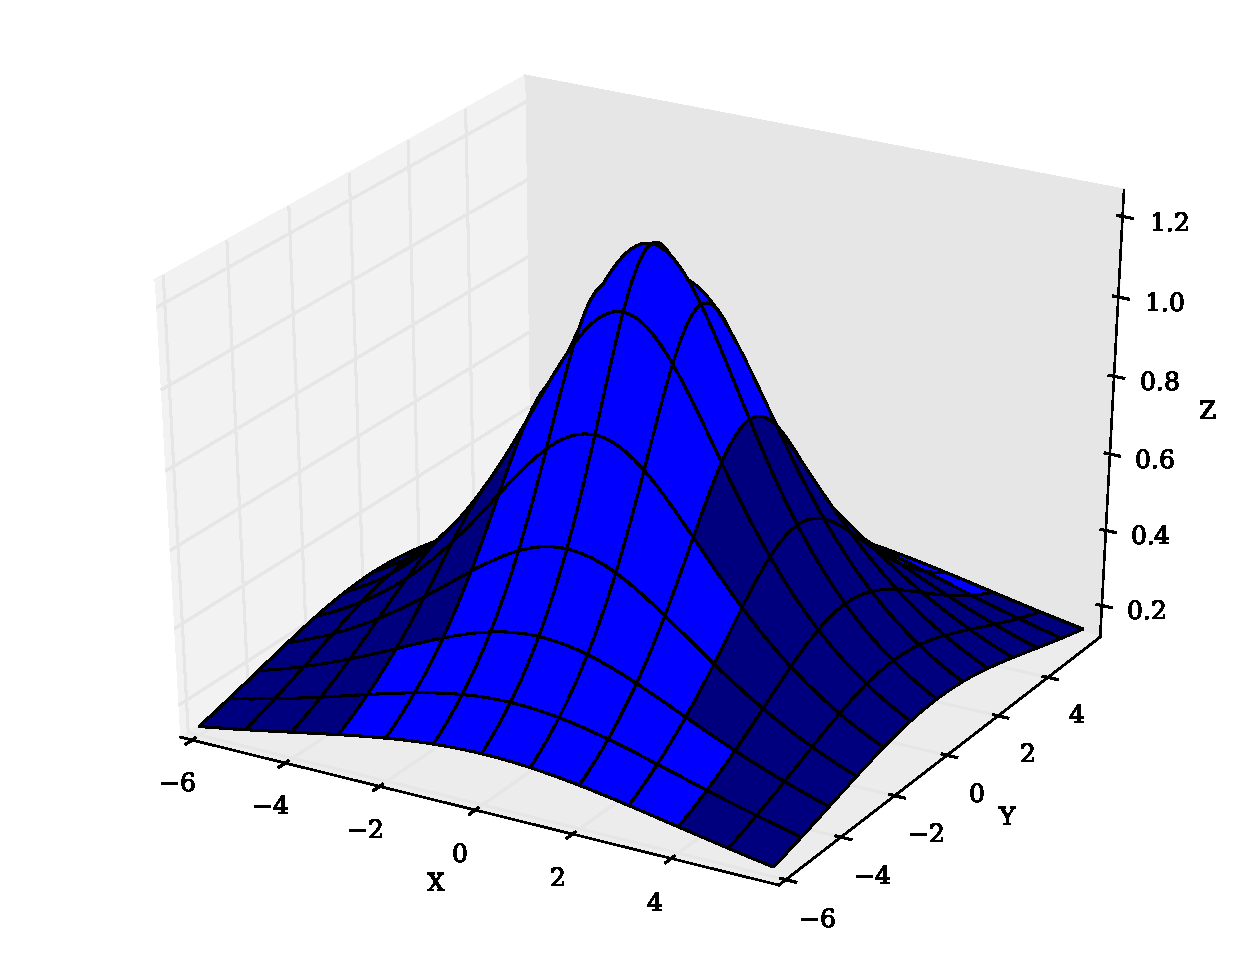
\includegraphics[width=5in]{figures/matplotlib9.eps}

 In this example, we import the {\color{blue}axes3d} module from the {\color{blue}mplot3d} toolkit of {\color{blue}matplotlib}.  We create an {\color{blue}Axes3D} instance called {\color{blue}ax}  from the {\color{blue}figure} object,  {\color{blue}fig}.   {\color{blue}Axes3D} objects have lots of methods, one of which is  {\color{blue}plot\_surface}, which plots a wireframe surface on the meshgrid  {\color{blue}X,Y} of the data in  {\color{blue}g}.    Other methods are  {\color{blue}set\_xlabel()} and so on.   Note that when you try this example on your own computer, you can twirl the plot around to see it from various perspectives.  You can save any of these with the little disk icon or with  {\color{blue}pylab.savefig()} as before.   
 
 To give you a flavor of what  {\color{blue}mlab} can do,  here is essentially the same code, but using functions from {\color{blue}mayavi.mlab}: 
 
{\singlespacing \color{blue} \begin{verbatim}
#!/usr/bin/env python
import numpy
from enthought.mayavi import mlab
def g(X,Y):
    G=6.67e-11 # grav constant in Nm^2/kg^2 (SI)
    R=2. # radius in meters
    drho=500 # density contrast in kg/m^3
    h=numpy.sqrt(X**2+Y**2)
    return 1e8*(G*4.*numpy.pi*R**3.*drho)/(3.*(h**2+z**2))
z=3. # depth of burial
X,Y=numpy.mgrid[-2.*z:2.*z:0.1,-2.*z:2.*z:0.1]
mlab.figure(bgcolor=(1,1,1))
s=mlab.surf(X,Y,g)
mlab.show()
\end{verbatim}}


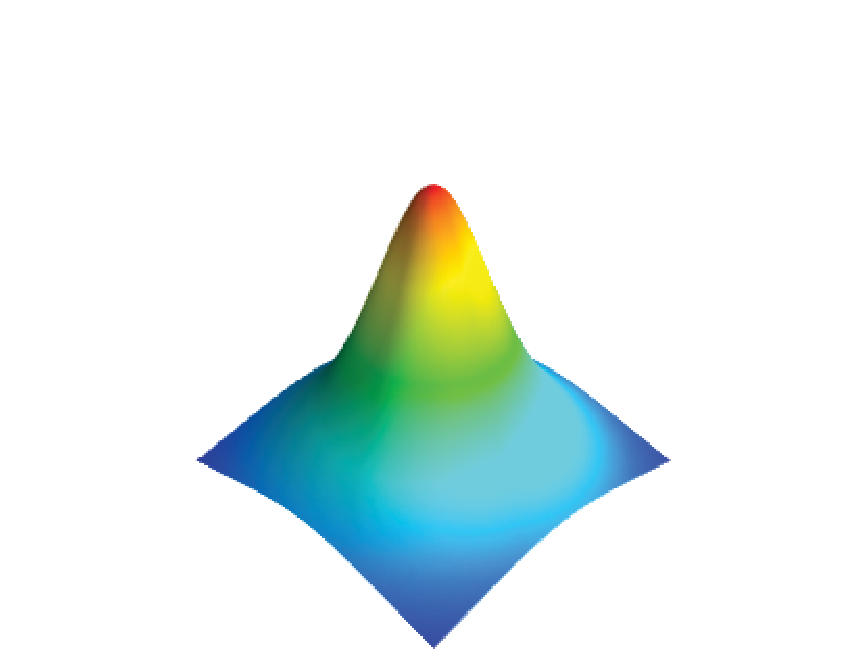
\includegraphics[width=5in]{figures/mlab.eps}

The call to  {\color{blue}mlab.figure} creates a figure instance instance with the background color (bgcolor) set to white.  In {\color{blue}mlab}, color gets set with the familiar r,g,b but here the colors run from 0 (black) to 1 (full strength), so a color of (1,1,1) is white, (1,0,0) is red, and so on.  The default is for a black background.  Then the surface gets drawn with a call to {\color{blue}mlab.surf()}.

There are lots more 3D plotting functions available in the two packages described here. To whet your appetite, I've picked out a few:  



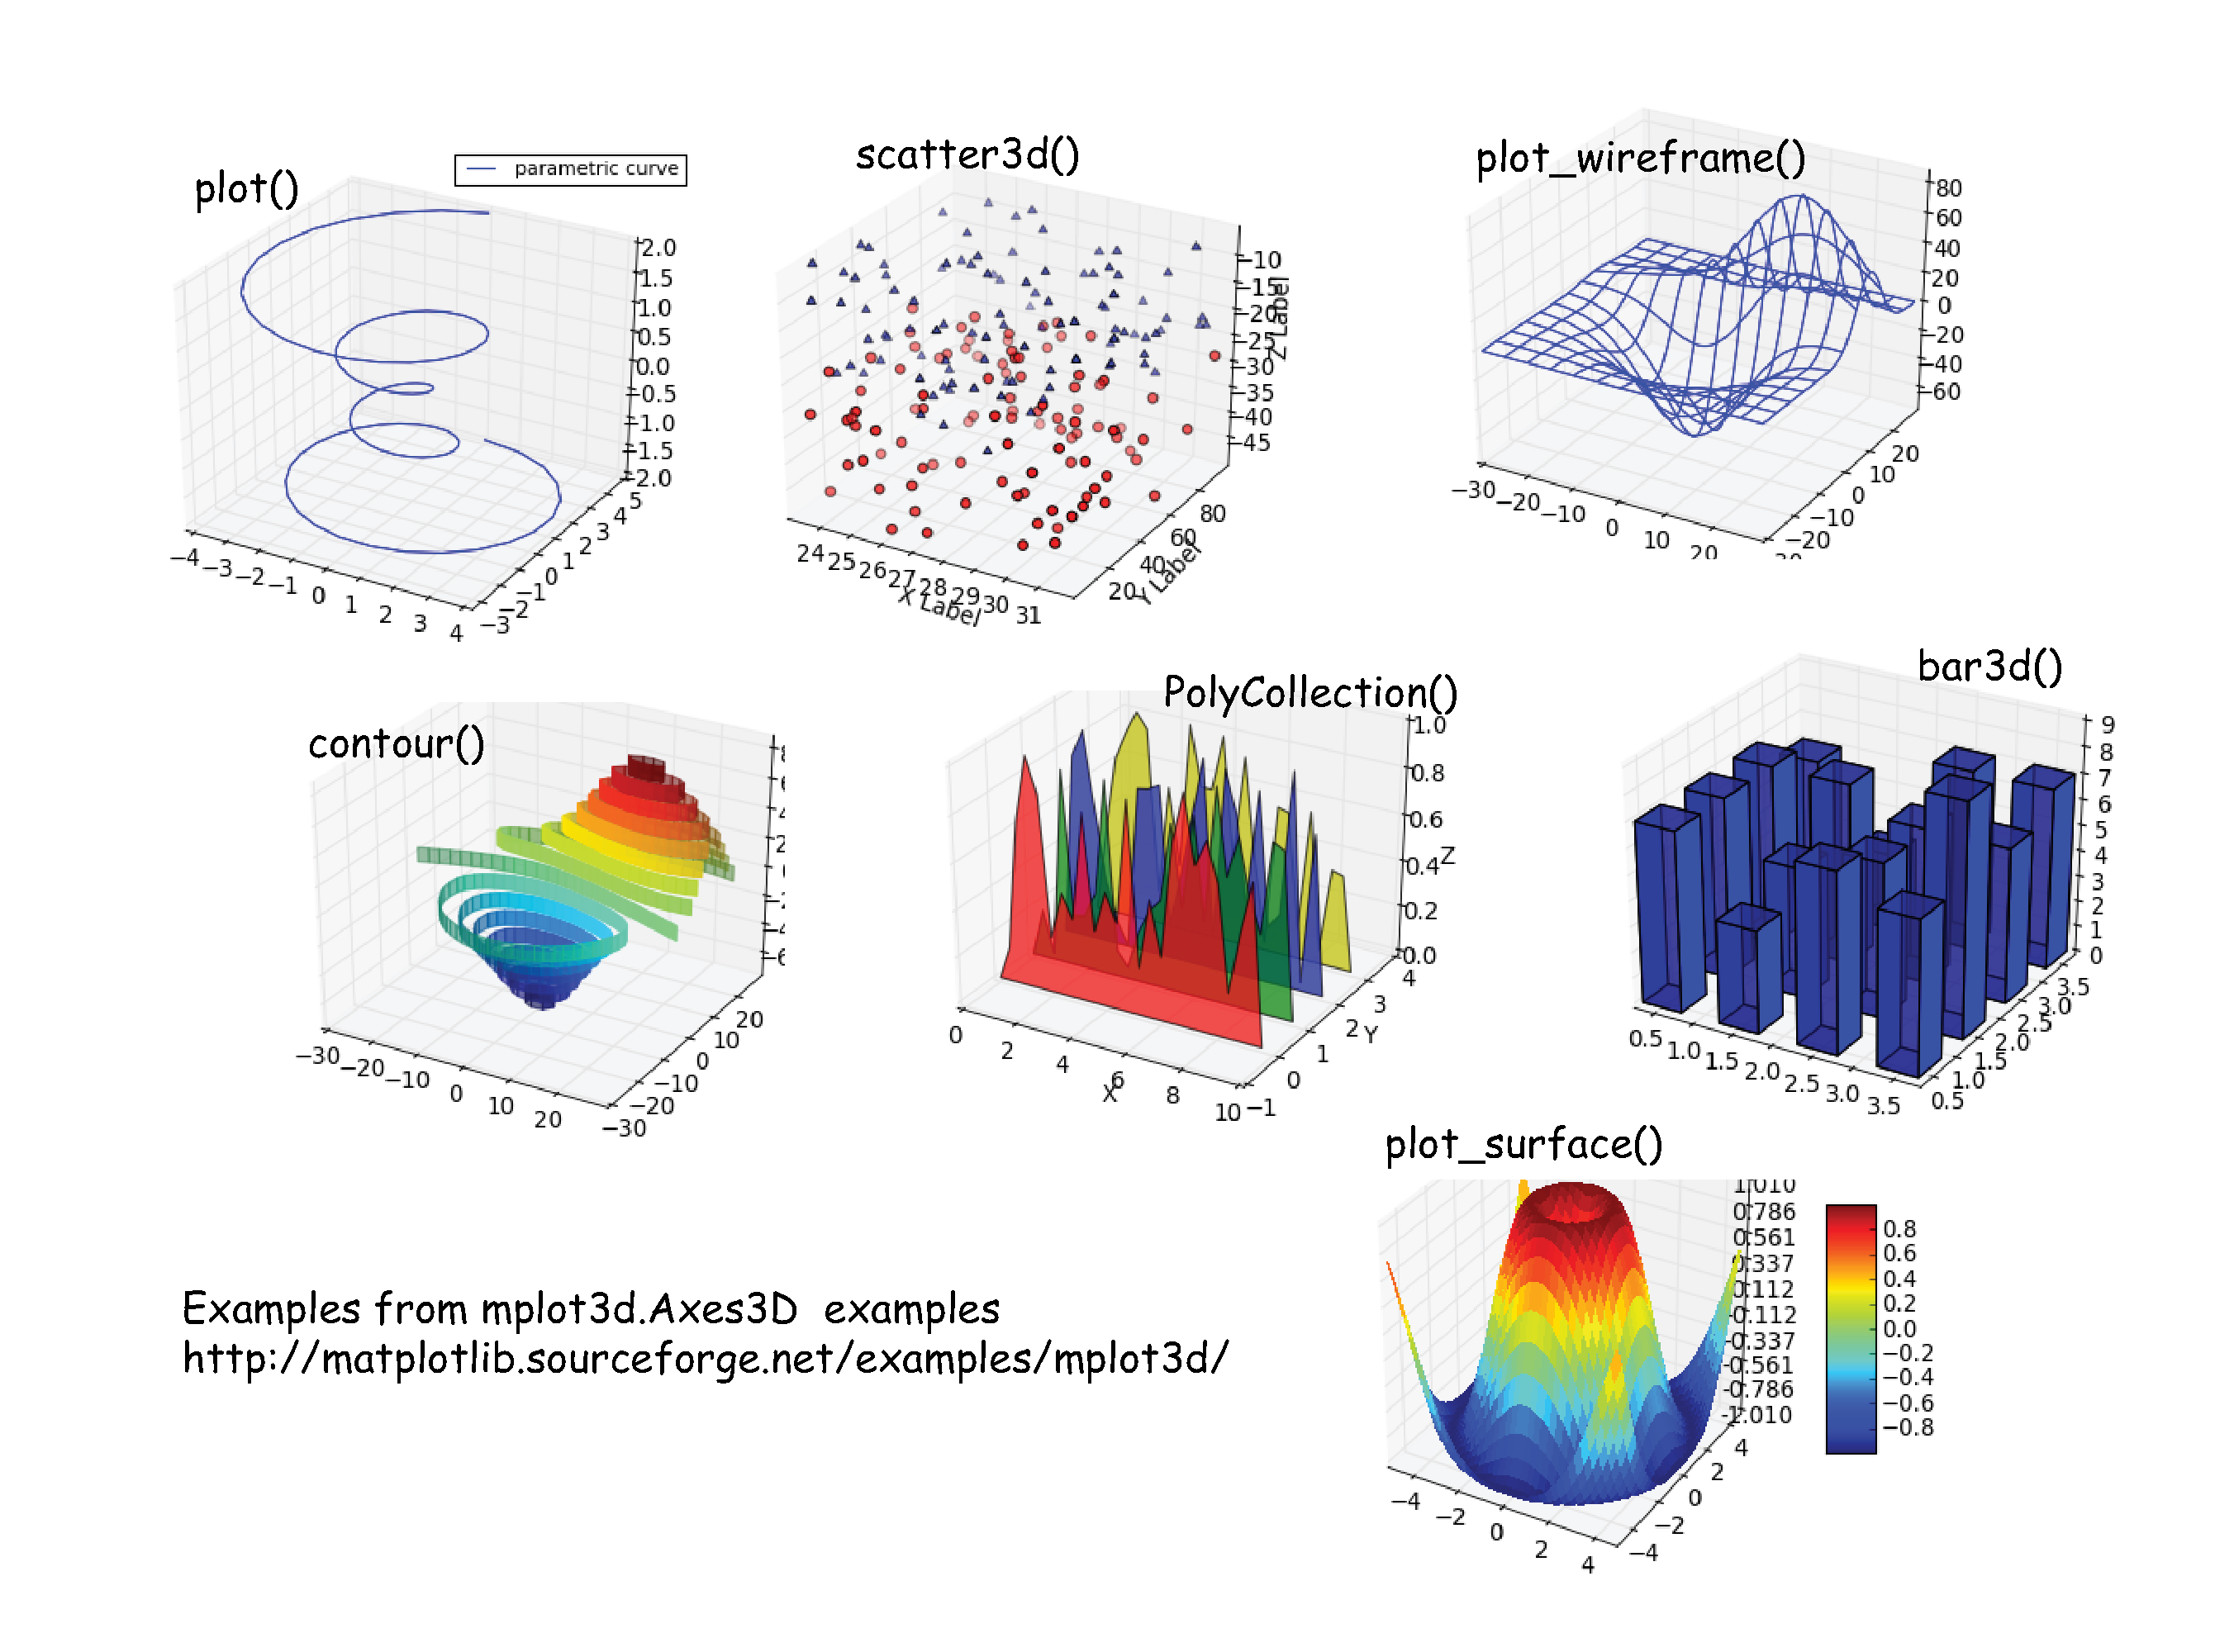
\includegraphics[width=4.5in]{figures/mplot3d-examples.eps}





\includegraphics[width=4.5in]{figures/mlab-examples2.eps}

\eject

Here are some considerations for you to help you decide which way you want to go: 

\centerline{mplot3d versus mlab}


\begin{tabular}{l|l}
\hline
mplot3d (matplotlib)  & mlab (mayavi)\\
\hline
Pros: & Pros:\\
\hline
mplot3d is a natural extension of pylab &  Prettier\\
 it is easier to learn & Interactivity\\
 pylab functions work for mplot3d too & More functions\\
 & Can be animated :)\\
\hline
Cons & Cons\\
\hline
 Limited plotting styles &no svg output \\
 & ps and eps are buggy\\
 & slower\\
& harder to learn for pylab masters\\
\hline
\end{tabular}




\subsection{Geoscience applications}
%%\vskip -.35in


There wouldn't be much point in learning how to program in a geoscience class if there were no practical applications.  In this section I will very briefly point out a few ways beyond the obvious X,Y plots and maps that you have already encountered.  

\subsubsection{Lines of flux}

Professor R.L.  Parker (our hero and professor emeritus of the SIO department) wrote a Fortran (f77) program called `force.f'. This was a slight modification of his   `magmap'  program that calculates magnetic field vectors given a geomagnetic reference model (see Bob's software website http://igppweb.ucsd.edu/$\sim$parker/Software/).  The program   force.f  has disappeared from Professor Parker's website in the mean time but is available on the class website at:
 
 http://mahi.ucsd.edu/class233/force.zip
 
\noindent  You run it with a session like this:


 it creates a file draws the magnetic lines of flux from the core outward and saves the data to a file like this:
 
 {\singlespacing \color{red}\begin{verbatim}
 % force
 \end{verbatim}}

 {\color{blue}\begin{verbatim} 
 
                    =================
 
Enter commands for spherical harmonic coefficients (? for help)
 \end{verbatim}}

 {\singlespacing \color{red}\begin{verbatim}
igrf 2005
lines 200
radius 0.547
output lines.f05
exec
\end{verbatim}}
 {\singlespacing \color{blue}\begin{verbatim} 
     ===================
     igrf 2005                                                                  
     lines 200                                                                  
     radius 0.547                                                               
     output lines.f05                                                           
     ===================
      
 Field evaluated for IGRF  2005
 Equatorial radius (km)   6378.170
 Polar radius      (km)   6356.910
 Reference radius  (km)   6371.200
 Evaluation r/a              0.547
 Maximum degree of accepted coefficients:   13
 Coefficients normalized to radius:  0.54700
 New field-line file opened in: lines.f05 
Initial and terminal points
    0.047   -0.049    0.998    0.054   -0.040    0.998
   -0.071    0.066   -0.995    0.532    0.164   -0.831
    0.226    0.217   -0.950    0.132    0.266   -0.955
   -0.272    0.686   -0.674   -0.160    0.516    0.842
    0.083    0.987   -0.139    0.123    0.945    0.302
    0.487   -0.385   -0.784    0.479   -0.382   -0.790
etc.
    0.016    0.856   -0.516    0.105    0.632    0.767
    0.642    0.316   -0.699    0.662    0.306   -0.684
 Field line coordinates written to lines.f05                                                               
 
                    =================
 
Enter commands for spherical harmonic coefficients (? for help)
\end{verbatim}}

{\singlespacing \color{red}\begin{verbatim}
quit
\end{verbatim}}

{\singlespacing \color{blue}\begin{verbatim}


                   Magmap run complete

\end{verbatim}}


\noindent  The red commands are typed by the user and then blue stuff is the program response.  This will create an output file {\color{blue}lines.f05} which looks something like this:
 
{\singlespacing \color{blue} \begin{verbatim}
    0.047   -0.049    0.998    1.000
    0.054   -0.040    0.998    1.000
           2   50.00000       50.00000       50.00000    
   -0.071    0.066   -0.995    1.000
   -0.054    0.070   -1.005    1.009
\end{verbatim}}

The first three columns are $x,y,z$ on a magnetic flux line and the fourth is $R$ in units of core mantle boundary radii. 
Each field line is separated from the rest by an entry with the number of points in the previous line and 3 ``50.000''s
Some of the field lines go WAY out in space (100 CMB radii); we'll come back to this later.

 Parker also provided a script ({\color{blue}look}) which chops off the parts of the lines that are more than 4 radii away, projects the 3D lines onto a plane specified by the user and saves the data in a new file.
It also invokes Parker's most famous program {\bf plotxy} (which IS available on his website). Plotxy produces a postscript file {\bf mypost}.  When run with the command {\color{blue}look 45 75 < lines.f05}, we get: 

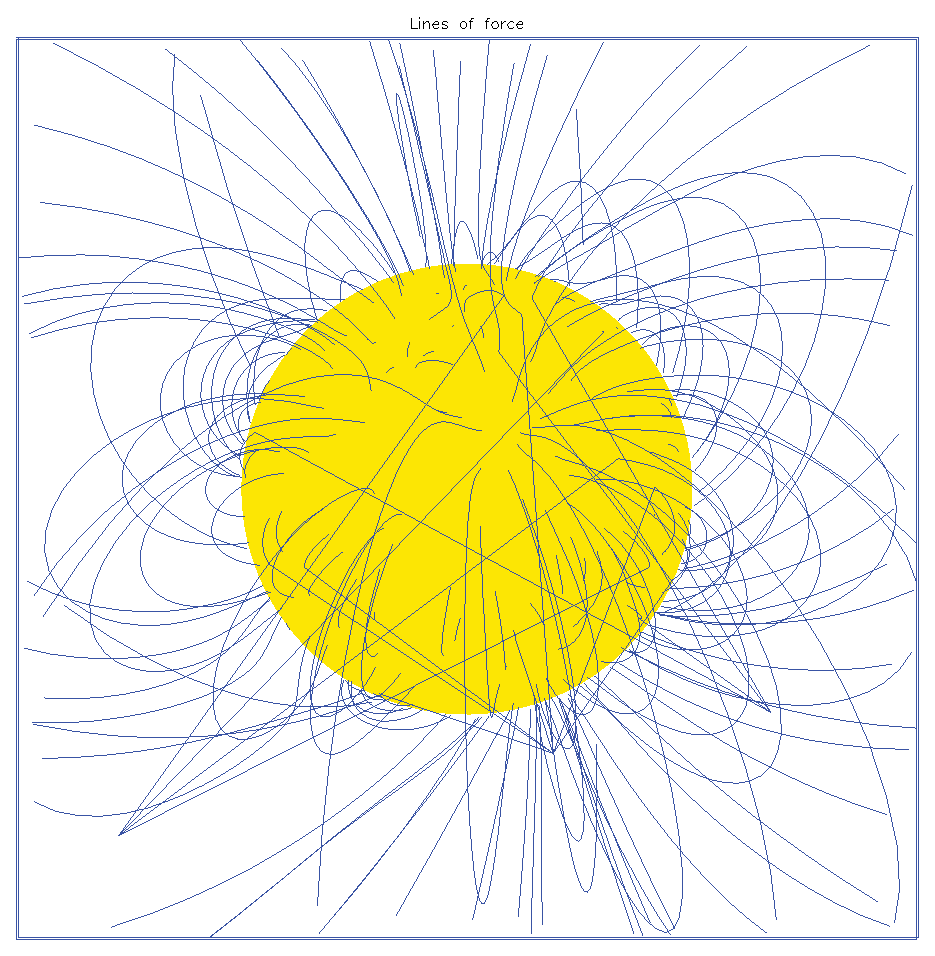
\includegraphics[width=4in]{figures/force.eps}

The thought occurs, wouldn't this look cool in 3D? Here is a little script inspired by the {\color{blue}plot3d()} example from the {\color{blue}Mlab} gallery.  

{\singlespacing \color{blue} \begin{verbatim}
#!/usr/bin/env python
import numpy as np
from enthought.mayavi import mlab
lines=np.fromstring(open('lines.f05').read(),dtype=float,sep=' ')
Xs,Ys,Zs,Rs=lines[0:-4:4],lines[1:-3:4],lines[2:-2:4],lines[3:-1:4]
line=0
lx,ly,lz,lr=[],[],[],[]
mlab.figure(bgcolor=(1,1,1)) # sets the background to white
while line<len(Xs):
    if Rs[line]<5: # truncates far away field lines
        lx.append(Xs[line])
        ly.append(Ys[line])
        lz.append(Zs[line])
        lr.append(Rs[line])
    elif Rs[line]>=5 and Ys[line]!=50.: # detects the 50's
        while Rs[line]>5 and Rs[line]!=50:
            line+=1
        x,y,z,r=np.array(lx),np.array(ly),np.array(lz),np.array(lr)
        mlab.plot3d(x,y,z,r,colormap='Spectral') 
        lx,ly,lz,lr=[],[],[],[]
    if Ys[line]==50. and line<len(Rs):
        x,y,z,r=np.array(lx),np.array(ly),np.array(lz),np.array(lr)
        mlab.plot3d(x,y,z,r,colormap='Spectral') 
        lx,ly,lz,lr=[],[],[],[]
    line+=1
mlab.show()
\end{verbatim}}

which produces something like this (but in 3D you can wiggle it around - much more fun!):

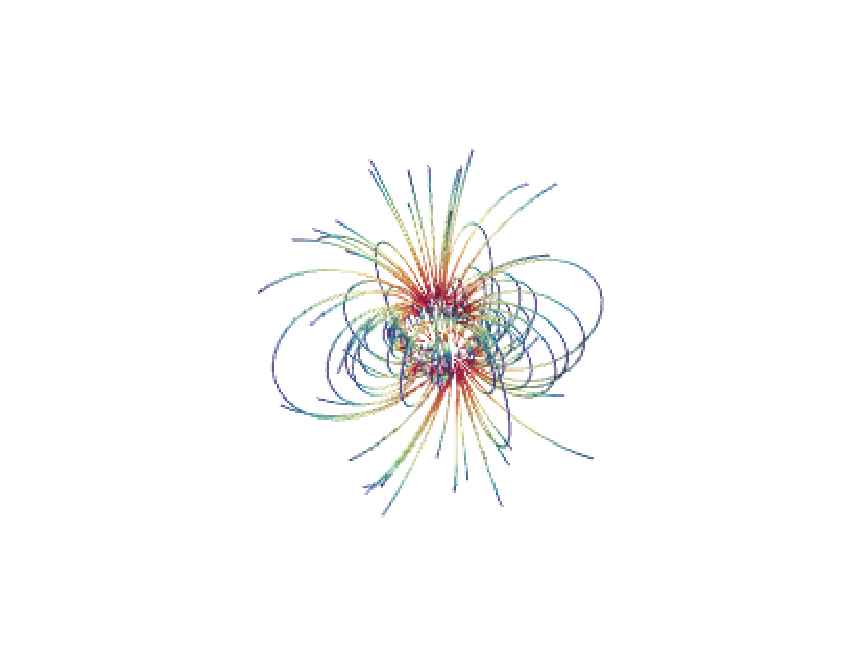
\includegraphics[width=4in]{figures/view_force.eps}

%

%\subsection{A closer look at plot3d}
%%%\vskip -.35in
%from the website:

%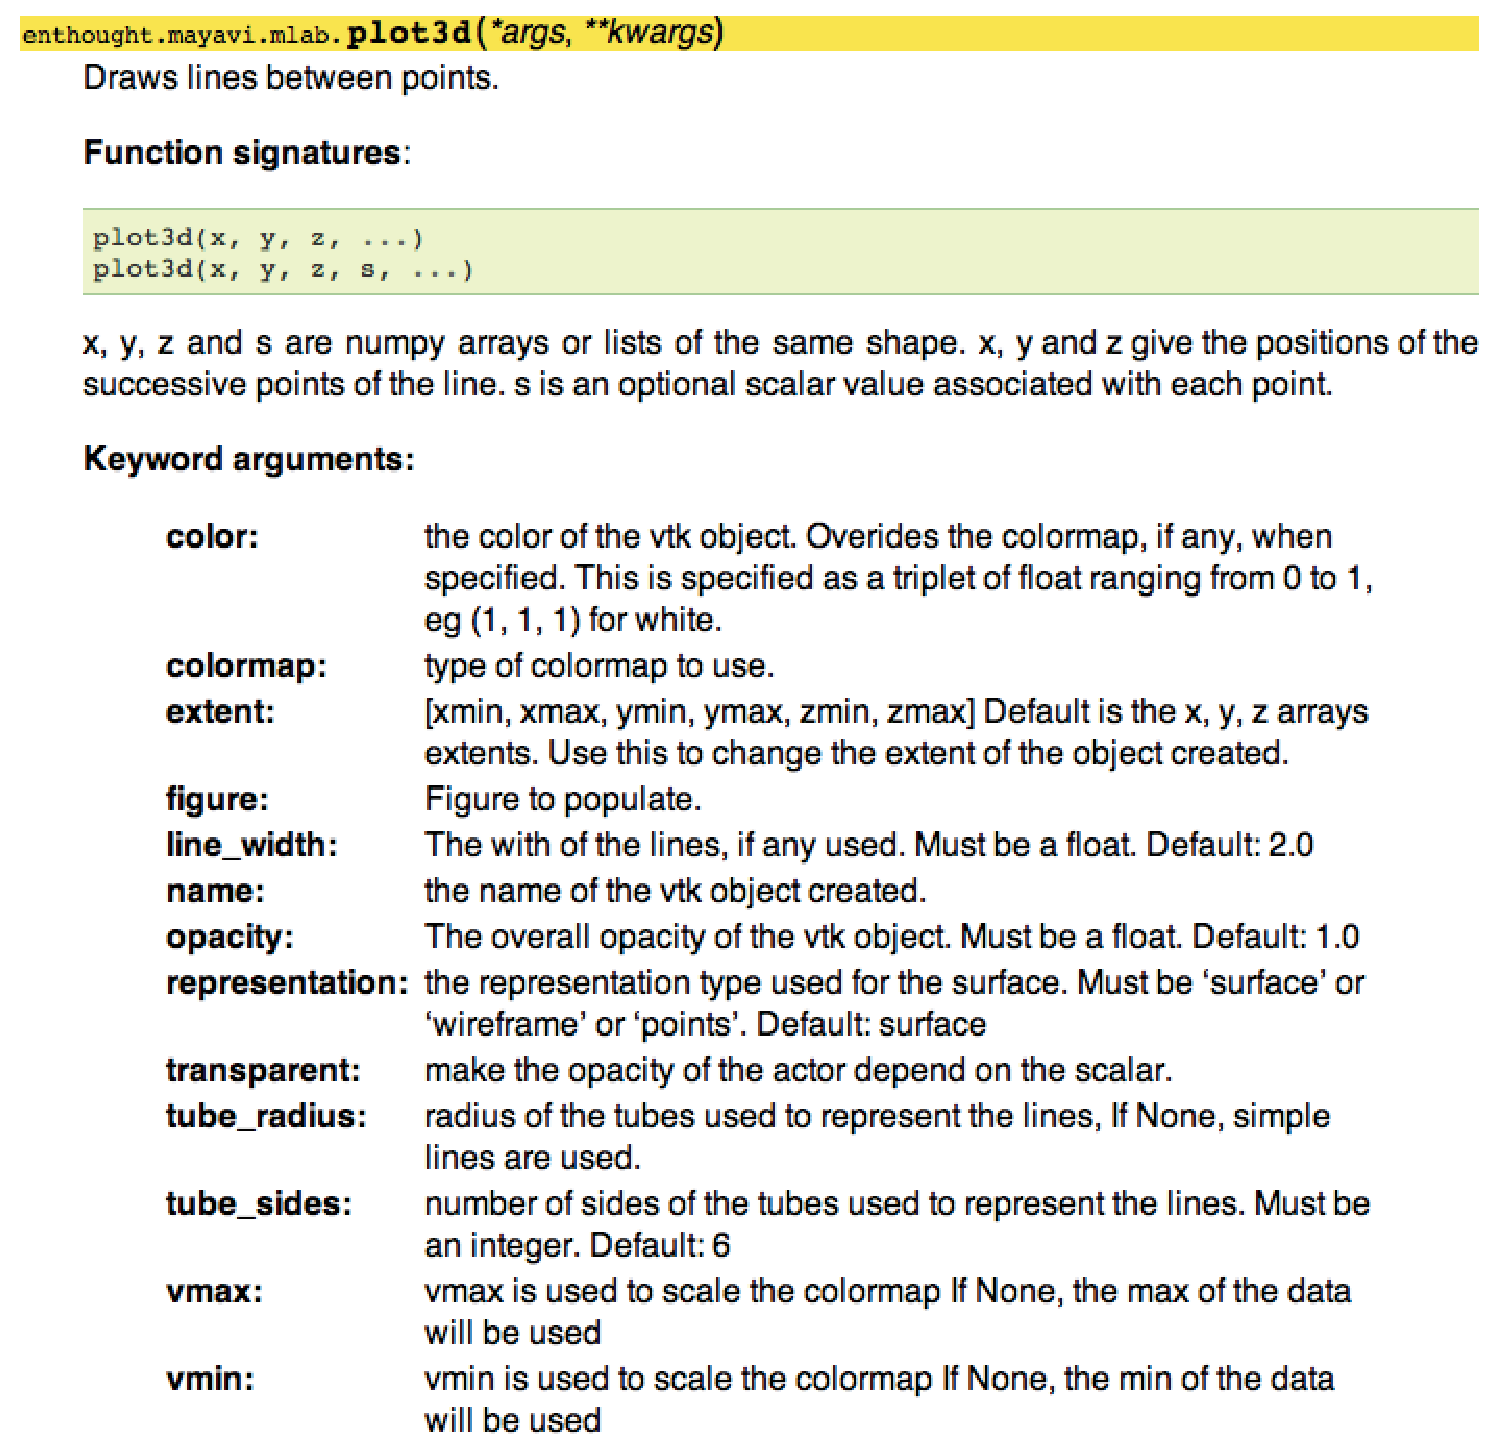
\includegraphics[scale=.3]{figures/plot3d-doc.eps}

%
%\subsection{Spherical harmonics}
%%%\vskip -.35in
%{%\small \baselineskip 0pt
%{\singlespacing \color{blue} \begin{verbatim}
%#!/usr/bin/env python
%from enthought.mayavi import mlab
%import numpy as np
%import sys
%from scipy.special import sph_harm
%n,m=int(sys.argv[1]),int(sys.argv[2])
%r = 0.3
%phi, theta = np.mgrid[0:np.pi:101j, 0:2*np.pi:101j]
%x = r*np.sin(phi)*np.cos(theta)
%y = r*np.sin(phi)*np.sin(theta)
%z = r*np.cos(phi)
%s = sph_harm(m, n, theta, phi).real
%mlab.mesh(x, y, z, scalars=s, colormap='jet')
%s[s<0]*=0.97
%s /= s.max()
%mlab.mesh(s*x+1, s*y, s*z, scalars=s, colormap='Spectral')
%mlab.show()
%\end{verbatim}}
%}

%%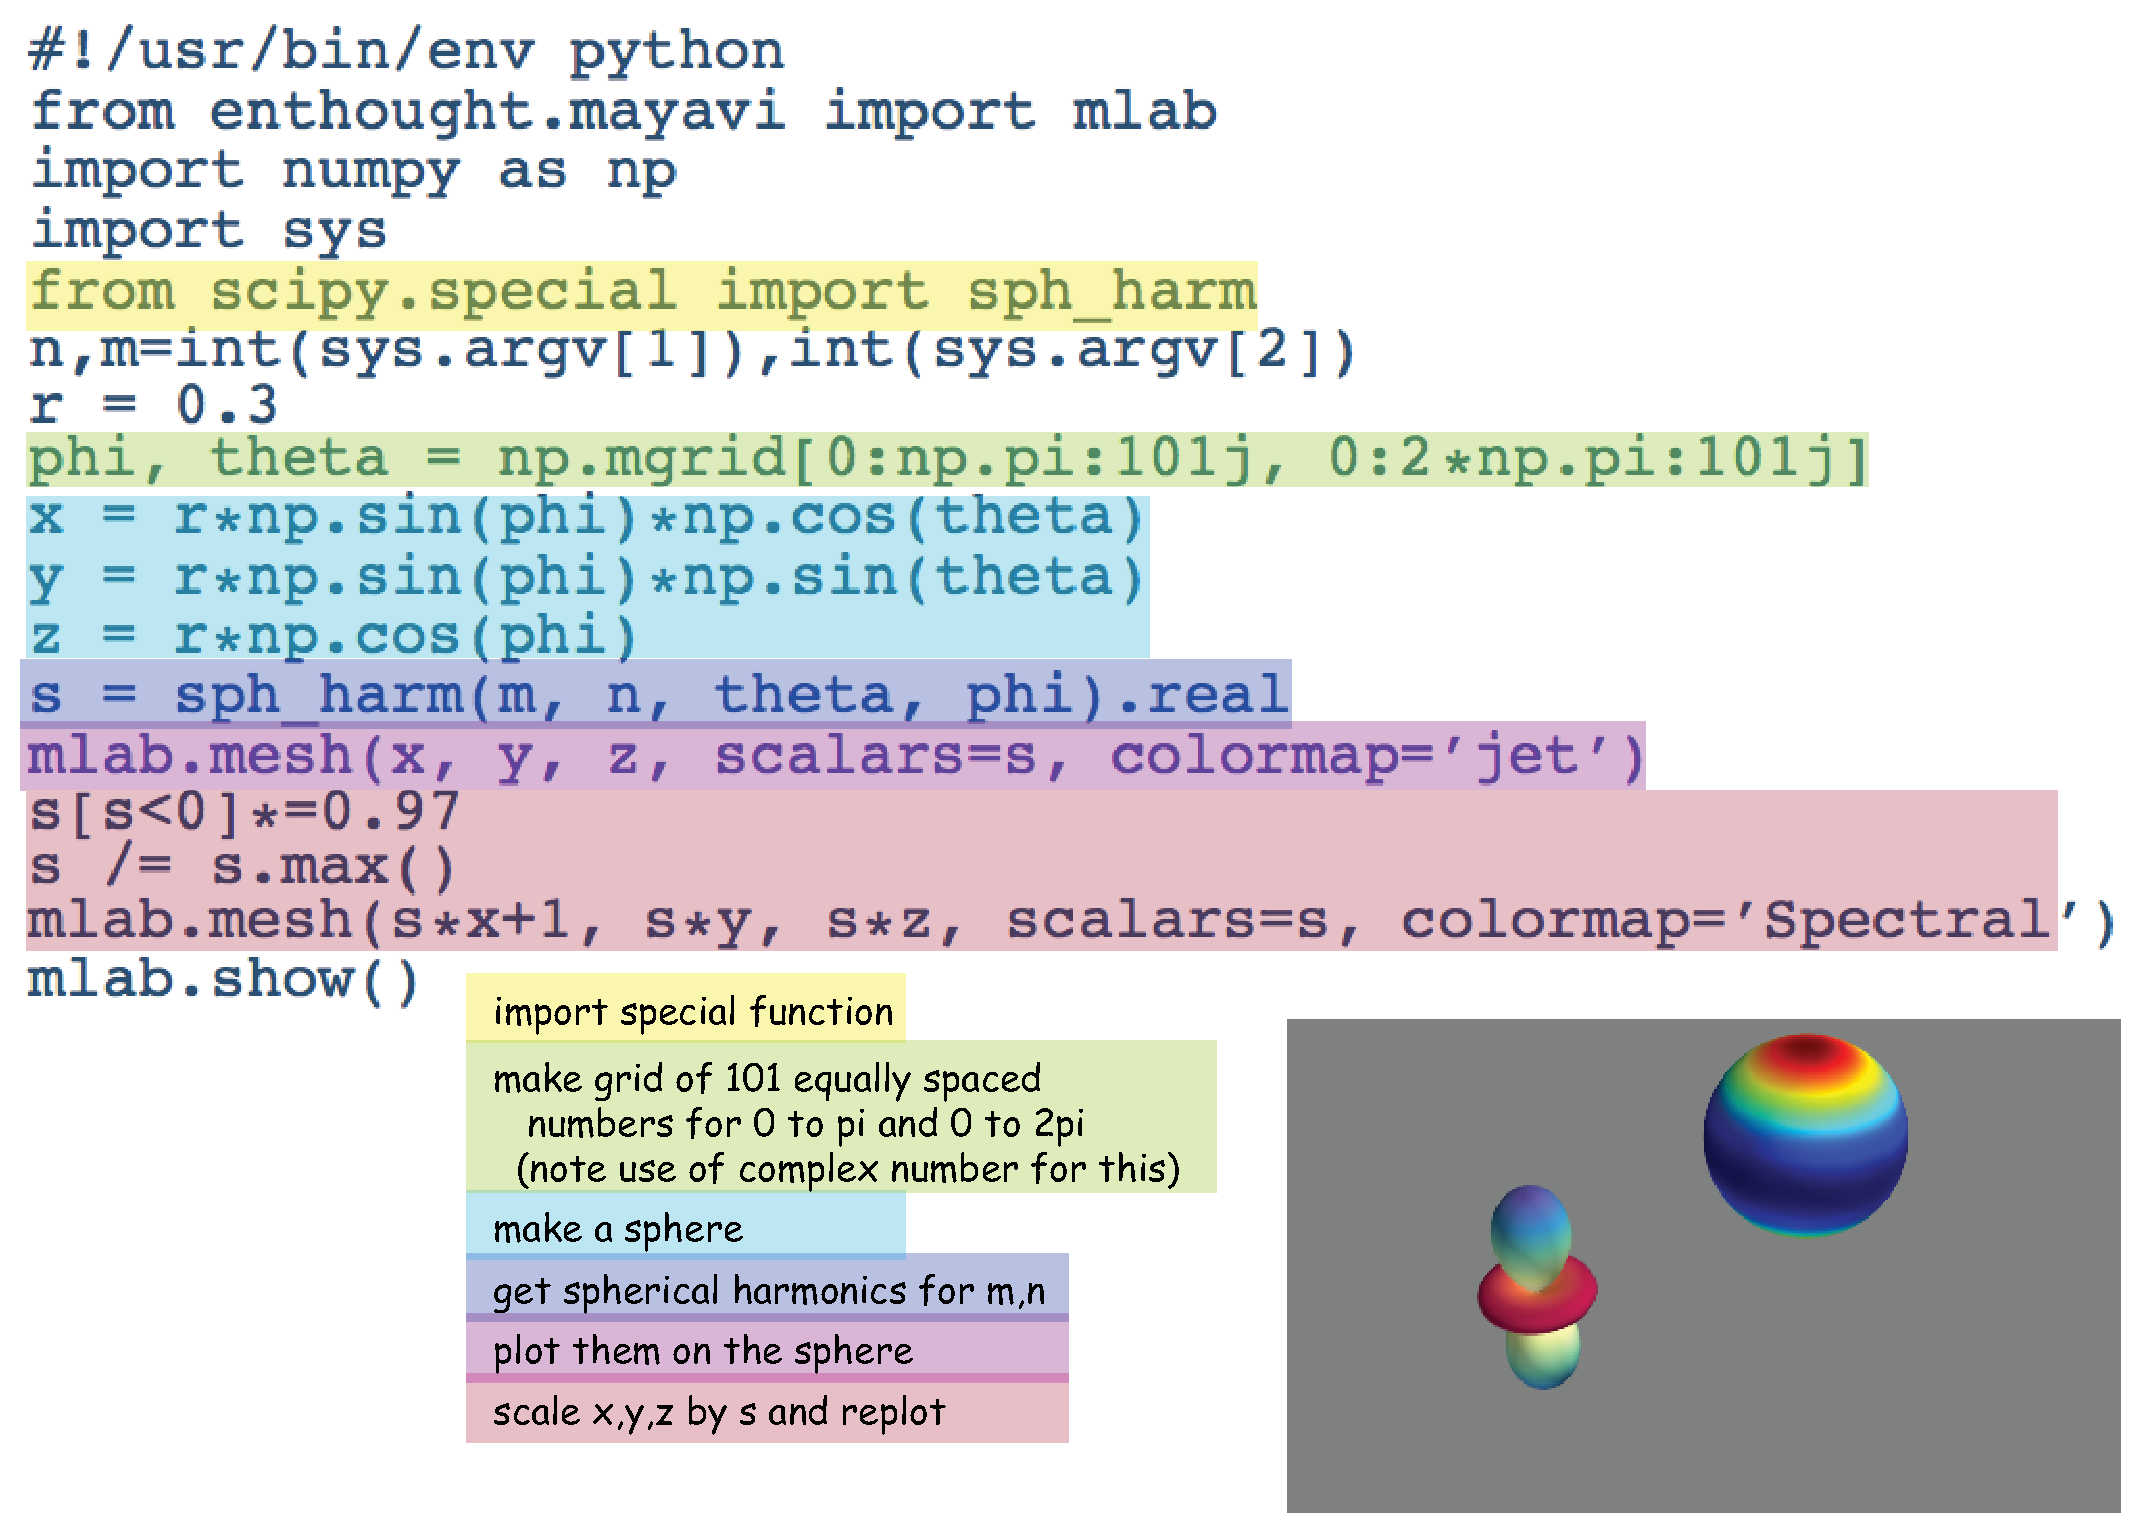
\includegraphics[scale=.25]{figures/mesh.eps}

%run mesh.py 2 0 for axial quadrupole

%




\subsubsection{Eigenvectors}

Linear algebra has a lot of applications in the geosciences.  One of the most useful tricks is to calculate what are called ``eigenparameters''.  Say you have a bunch of points and want to calculate a best-fit line through them - but they are in three dimensions.  Or you want a best fit plane, say the fault surface through a bunch of earthquakes.  Or you want to know the principal axis of the  moment of inertia tensor.  Or the orientations of a stress or strain tensors.  Or the preferred orientation of mineral grains or clasts in a sedimentary deposit.  Or the directions of the  anisotropy of just about anything.
And the list goes on.  Here is an example that finds the eigenvectors and eigenvalues of what is called the covariance matrix of a bunch of 3D points. These could be the end points of unit vectors (directions), or point masses in space, for example.



{\singlespacing \color{blue} \begin{verbatim}
#!/usr/bin/env python
import numpy
from numpy import linalg
from enthought.mayavi import mlab
dat=open('points.xyz','rU').readlines()
x,y,z=[],[],[]
for line in dat:
    rec=line.strip('\n').split()
    x.append(float(rec[0]))
    y.append(float(rec[1]))
    z.append(float(rec[2]))
X,Y,Z=numpy.array(x),numpy.array(y),numpy.array(z)
T=numpy.array([[numpy.sum(X*X),numpy.sum(X*Y),numpy.sum(X*Z)],\
    [numpy.sum(Y*X),numpy.sum(Y*Y),numpy.sum(Y*Z)],\
    [numpy.sum(Z*X),numpy.sum(Z*Y),numpy.sum(Z*Z)]])
evals,evects=linalg.eig(T)
print 'principal axis: ',evects.transpose()[0], ' with variance of ',evals[0]
print 'major axis: ',evects.transpose()[1], ' with variance of ',evals[1]
print 'minor  axis: ',evects.transpose()[2], ' with variance of ',evals[2]
pv=evects.transpose()[0]*3.
mlab.figure(bgcolor=(1,1,1))
mlab.points3d(X,Y,Z,color=(0,0,0),scale_factor=0.25,opacity=.5)
mlab.outline(color=(.7,0,0))
mlab.plot3d([pv[0],-pv[0]],[pv[1],-pv[1]],\
   [pv[2],-pv[2]],tube_radius=0.1,color=(0,1,0))
mlab.show()
\end{verbatim}}


{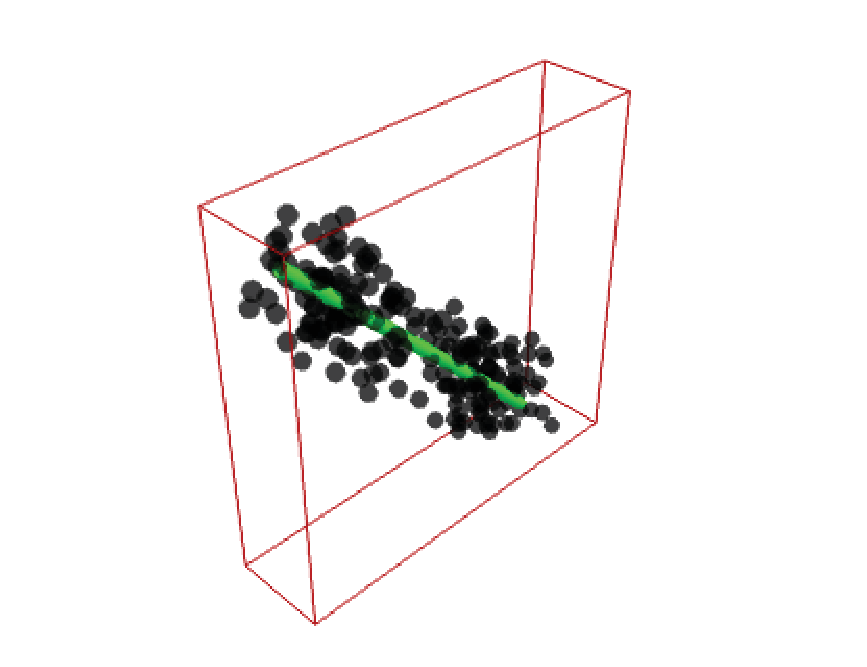
\includegraphics[width=4in]{figures/points.eps}}

This script opens a  file called {\color{blue}points.xyz} which looks like this:

{\singlespacing \color{blue}\begin{verbatim}
1.4844e+00 5.9620e-02 2.2025e+00
1.6928e+00 4.7284e-02 1.0015e+00
9.7893e-01 -2.7332e-01 6.6763e-01
1.1998e+00 -1.9863e-01 5.1122e-01
7.6767e-01 2.1443e-02 7.9248e-01
1.5916e+00 9.7349e-02 1.8151e+00
1.4537e+00 1.3741e-01 2.1087e+00
etc.
\end{verbatim}}

\noindent  It then parses the data into lists of floating point  variables.  These get turned into arrays.  
Then the sums of the products and squares  get put into a coherence matrix of the form:

$$ \pmatrix{\sum x^2&\sum xy &\sum xz \cr
    \sum xy &\sum y^2 &\sum yz \cr 
  \sum xz&\sum yz&\sum z^2 \cr}.
$$

\noindent The function {\color{blue}linalg.eigs()} returns the eigenvectors and eigenvalues of this ``T'' matrix.  The largest (principal) eigenvalue corresponds to the principal eigenvector and is the axis along which the variance (spread) is the greatest.  The minor eigenvector corresponds to the axis along which the variance is least.   One ``feature'' of this function is that the coordinates of the eigenvectors are along axis 0, so are the first column of the evects array:

{\singlespacing \color{blue}\begin{verbatim}
evects=
[[ 0.70464008 -0.70917141  0.02362748]
 [-0.001072    0.03223454  0.99947976]
 [ 0.70956409  0.70429883 -0.02195351]]
 \end{verbatim}}
 
 \noindent   That is why to print out the vectors:
 
 {\singlespacing \color{blue}\begin{verbatim}
% points.py
principal axis:  [ 0.70464008 -0.001072    0.70956409]  with variance of  733.172618519
major axis:  [-0.70917141  0.03223454  0.70429883]  with variance of  30.501077006
minor  axis:  [ 0.02362748  0.99947976 -0.02195351]  with variance of  8.55431560739
\end{verbatim}}


\noindent   I take the transpose. 

 The principal eigenvector gets assigned to the array {\color{blue}pv}.   he function {\color{blue}points3d} plots the points a nice shade of grey (opacity low). {\color{blue}mlab.outline(color=(.7,0,0))} puts a red box around the figure and {\color{blue}mlab.plot3d} plots the principal eigenvector as a green tube.  Nice.
 



\vfill
\end{document}
